\documentclass[12pt,twoside]{book}
\usepackage[T1]{fontenc}
\usepackage{color}
\usepackage{amsmath}
\usepackage{amssymb}
\usepackage[toc,page,title,titletoc,header]{appendix}
\usepackage{babel}
\usepackage{times}
\usepackage{subcaption}
%\usepackage{kpfonts}
\usepackage{setspace}
\setstretch{1.5}
\usepackage{fancyhdr}
\usepackage[clearempty]{titlesec}
\usepackage{caption}
\usepackage{verbatim}
\usepackage{lastpage}
\usepackage{graphicx}
\usepackage[margin=25mm]{geometry}
\newtheorem{theorem}{Théorème}
\newtheorem{algorithm}{Algorithme}
%\title{ETUDE ET REALISATION D'UN ANNULATEUR D'ECHO SONORE MIXTE} 
%\author{\textsc{KRAME Kadurha David}}
\usepackage[colorlinks=true,breaklinks=true,linkcolor=blue]{hyperref}
%\date{Le 07 Janvier 2021}
\pagestyle{fancy}
\renewcommand{\headrulewidth}{0.4pt}
\renewcommand{\footrulewidth}{0.4pt}
\fancyhead[LE]{\leftmark}
\fancyhead[RO]{\rightmark}
\fancyhead[RE]{}
\fancyhead[LO]{}
\fancyfoot[C]{\thepage\hspace{1pt} sur \pageref{LastPage}}
\begin{document}
%\maketitle
\begin{titlepage}
%\begin{sffamily}
\begin{center}
\textsc{\LARGE UNIVERSITE LIBRE DES PAYS DES GRANDS LACS}\\[0.4cm]
\textsc{\LARGE ULPGL-Goma}\\[0.4cm]
\textsc{\Large B.P $ 368 $ GOMA / www.ulpgl.net}\\
\vspace{2pt}
\rule{0.5\linewidth}{2pt}
\vspace{0.5cm}\\
\textsc{\Large Faculté des Sciences et Technologies Appliquées}\\
\begin{center}
\includegraphics[scale=1]{logoUL.png}
\end{center}
\textbf{\Large Département de Génie Électrique et Informatique}\\
\vspace{10pt}
\begin{center}
\makebox[15cm]{\LARGE CONCEPTION D'UN FILTRE ANNULATEUR}
\makebox[15cm]{\LARGE D'ECHO SONORE MIXTE}
\end{center}
\vspace{35pt}
\hspace*{5cm}\begin{minipage}{0.7 \textwidth}
\begin{flushleft}\large
Travail de fin de cycle présenté en vue de l'obtention du diplôme de Graduat en Sciences Appliquées.\\
\vspace{7pt}
Présenté par : \textbf{\textsc{KRAME KADURHA David}}\\
Directeur : DI.Dr.Tech. \textsc{Alain AKWIR NKIEDIEL}\\
Encadreur : Ass$ 2 $.Ing. \textsc{Dieudonné MUSONGYA BISIMWA}
\end{flushleft}
\end{minipage}
\hrulefill
\begin{center}
\vspace{35pt}
\fbox{\textbf{\Large Année académique   $ 2019-2020 $}}
\end{center}
\end{center}
%\end{sffamily}
\end{titlepage}

\renewcommand{\bibname}{Bibliographie}
\renewcommand{\chaptername}{Chapitre}
\renewcommand{\appendixtocname}{ANNEXES}
\renewcommand{\appendixpagename}{ANNEXES}
\renewcommand{\contentsname}{Table des matières}
\renewcommand{\listfigurename}{Liste des figures}
\frontmatter
\chapter*{DÉDICACES}\addcontentsline{toc}{chapter}{DÉDICACES}
A ma chère tante Catherine FEZA
\chapter*{REMERCIEMENTS}\addcontentsline{toc}{chapter}{REMERCIEMENTS}
$ _{} $ $ _{} $ $ _{} $ $ _{} $ $ _{} $Nous remercions en premier Dieu pour la guidance qu'il ne cesse de nous accorder. En second lieu, nos remerciements s'adressent à notre université, l'ULPGL, qui nous a encadré durant cette partie de notre quête des connaissances.\\
$ _{} $ $ _{} $ $ _{} $ $ _{} $ $ _{} $Nos remerciements les plus sincères alors à notre directeur, le Professeur BARAKA MUSHAGE Olivier, et notre encadreur, le Msc. KAMBALE WAMUHINDO Abednego, pour le suivi humble, patient et attentif qu'ils nous ont accordé durant ce travail.\\
Nous remercions aussi tous nos professeurs, en particulier ceux qui nous ont fortement inspiré, dont notre directeur ainsi que les professeurs Alain AKWIR,  LOHALO Rostha et NKUMBI Mwamba.\\
$ _{} $ $ _{} $ $ _{} $ $ _{} $ $ _{} $Nos remerciements très reconnaissants à notre mère BALIBUNO NZIGIRE Charlotte et à notre oncle BALIBUNO Juvénal, pour le soutient tant moral, matériel qu'affectif qu'ils ne cessent de nous accorder.\\
Nous adressons également nos remerciements les plus sincères à la Sr Catherine FEZA, à Bijoux NAMWESI, BAKONDJO Pontien, Irène IRAGI, WILLY Miruho, BAENI Innocent, Labii KADURHA, Georgette KADURHA et nos oncles Marcellin BALIBUNO, Christian ACIZA CUBAKA, Akonkwa BALIBUNO, Bisimwa BALIBUNO, Mushagalusa ZAGABE, Aganze BALIBUNO et Bernardin BWIRABUCIZA pour le soutien.\\
$ _{} $ $ _{} $ $ _{} $ $ _{} $ $ _{} $Nous remercions aussi tous ceux dont l'existence contribue énormément à notre bien-être, pensant à Joëlle ANSIMA, Daniel KADURHA, Emmanuella MUSIMWA,Generose ABEKA, Florence CINAMA, Christelle MIRUHO, Patricia OLINABABO, Alohn SHETEBO, Carine SHETEBO, Christian RUBONEKA, Jehiel BABUYA, Jadhiel LUKOO, MUBARUZA Hugues, ILOMBE Bertrand, Wen KAMUNTU et René VUNINGA.\\
$ _{} $ $ _{} $ $ _{} $ $ _{} $ $ _{} $Nous remercions enfin nos amis et camarades, dont en particulier Styve EBASOMBA, Naomi MASASI, SOKI Claudette, KAMOLE Bruno, KAHASHI Yvan, Moise MUHESI, USHINDI Victoire, CIRHULWIRE Chrispin, Pierre MABILI, AMANI Lucien et tous les gens bienveillants que nous n'avons pas pu citer.
\begin{flushright}
\textbf{\textsc{KRAME Kadurha David}}
\end{flushright}

\chapter*{RÉSUMÉ}\addcontentsline{toc}{chapter}{RÉSUMÉ}
$ _{} $ $ _{} $ $ _{} $ $ _{} $ $ _{} $A l'ère du numérique, le texte est l'un des principaux moyens de communication et surtout de transmission des savoirs. En 2018, c'était environ $ 80\% $ des informations circulant sur le web. Mais, le temps étant une denrée rare, on voudrait avoir la possibilité d'accéder directement aux informations saillantes des textes, ou juste en avoir un aperçu global avant d'y consacrer du temps. D'où la nécessité d'un système de résumé automatique performant.
Dans ce travail, notre objectif est de mettre en place un système de résumé automatique performant. Pour cela, nous avons considéré à la fois le résumé abstractif et extractif, laissant le choix à l'utilisateur, selon ses besoins en information.
Pour le résumé extractif, nous avons considéré deux approches qui ont consisté à utiliser un module python dénommé \textit{gensim} pour la synthèse, puis un mélange de plusieurs algorithmes de synthèse que nous avons nommé \textit{merging}. Pour le résumé abstractif, nous avons opté pour les modèles du type \textit{transformer} car ce sont eux qui ont atteint jusqu'à présent les performances les plus élevées pour diverses tâches de traitement du langage naturel. Néanmoins, nous avons servi les \textit{transformers} utilisés pour la synthèse abstractive à travers un pipeline devant permettre l'amélioration des performances et l'augmentation du nombre de pages recevables.
A l'issu de nos expérimentations, nous avons trouvé que l'algorithme \textit{merging} était qualitativement plus performant que \textit{gensim}. Nous avons également enregistré une nette amélioration des résultats fournis par les \textit{transformers} une fois servis à travers le pipeline que nous avons proposé.
Ainsi, nous avons obtenu un système capable de restituer les résumés abstractifs ou extractifs des textes. Pour cela, nous avons mis en place une interface de pro\-gram\-ma\-tion des ap\-pli\-ca\-tions que les développeurs pourraient utiliser pour réaliser la syn\-thè\-se au\-to\-ma\-ti\-que dans leurs systèmes respectifs, nous avons im\-plé\-men\-té une application web qui exploite les services de cette interface mise au point et avons réalisé un modèle qui sera entrain d'être amélioré au fil de la collecte des couples texte-synthèse à travers notre système.\\
\underline{\textbf{Mots-clés}} : Intelligence artificielle, Encodeur-décodeur, Transformer, résumé automatique des textes, Python, Flask, JavaScript, ReactJS, ExpressJS.
\chapter*{SIGLES ET ABRÉVIATIONS}\addcontentsline{toc}{chapter}{SIGLES ET ABRÉVIATIONS}
\textbf{ALBERT}: A Lite BERT ,\\
\textbf{ANN}: Artificial Neural Network,\\
\textbf{API}: Application Programming Interface,\\
\textbf{BART}: Bidirectionnal and Auto-Regressive Transformer,\\
\textbf{BBC} : British BroodCasting Corporation,\\
\textbf{BD} : Base des Données,\\
\textbf{BERT}: Bidirectionnal Encoder Representations from Transformers,\\
\textbf{CNN} : Cable News Network,\\
\textbf{CSS} : Cascading Style Sheets,\\
\textbf{DUC} : Document Understanding Conference,\\
\textbf{GPT} : Generative Pretrained Transformer,\\
\textbf{GRU} : Gated Recurrent Unit,\\
\textbf{HTML} : HyperText Markup Language,\\
\textbf{LCS} : Long Common Sequence,\\
\textbf{LDA} : Latent Dirichlet Allocation,\\
\textbf{LSA} : Latent Semantic Analysis,\\
\textbf{LSTM} : Long Short-Term Memory,\\
\textbf{MML} : Masked Language Modelling,\\
\textbf{NER} : Named Entity Recognition,\\
\textbf{NLP} : Natural Language Processing,\\
\textbf{NLU} : Natural Language Understanding,\\
\textbf{NSP} : Next Sentence Prediction,\\
\textbf{POS} : Part Of Speech,\\
\textbf{REST} : REpresentationnal State Transfer,\\
\textbf{RNN} : Recurrent Neural Network,\\
\textbf{ROBERTA}: Robustly Optimized BERT Approach ,\\
\textbf{ROUGE} : Recall Oriented Understudy for Gisting Evaluation,\\
\textbf{RST} : Rhetorical Structure Theory,\\
\textbf{SCU} : Summary Content Unit,\\
\textbf{SMS} : Short Message Service,\\
\textbf{SVD} : Singular Value Decomposition,\\
\textbf{T5} : Text-To-Text Transfer Transformer,\\
\textbf{TAC} : Text-Analysis Conference,\\
\textbf{TF-IDF} : Time Frequency Inverse Document Frequency,\\
\textbf{ULPGL} : Université Libre des Pays des Grands-Lacs,\\
\textbf{XSum} : Extreme Summarization,\\
\textbf{mBART} : multilingual BART,\\
\textbf{mT5} : multilingual T5.
\tableofcontents
\listoffigures

\mainmatter
\chapter*{INTRODUCTION GÉNÉRALE}\addcontentsline{toc}{chapter}{INTRODUCTION GÉNÉRALE}
\section{Contexte}
$ _{} $ $ _{} $ $ _{} $ $ _{} $ $ _{} $A l'ère du numérique, comme depuis l'invention de l'écriture, le texte est l'un des principaux moyens de communication et surtout, de transmission des connaissances.\\
Des livres aux SMS, en passant par diverses pages web, les données textuelles sont partout.\\
En $ 2018 $, il s'agissait d'environs $ 80\% $ de l'information qui circulait sur le web \cite{lamsiyah-etal-2018-resume}.\\
L'évolution de l'informatique continue à démontrer la possibilité de simplifier toujours grandement la vie de l'homme en automatisant de plus en plus l'accomplissement des tâches rébarbatives.\\
Certaines tâches comme celles liées explicitement à l'arithmétique semblent mieux se prêter à cette vague d'automatisation, les données numériques étant par essence celles prises en compte par les plateformes numériques.\\
$ _{} $ $ _{} $ $ _{} $ $ _{} $ $ _{} $Néanmoins, des transformations adéquates permettent de prendre en compte tout type de donnée, et le texte n'est pas exclu. C'est ainsi que, des avancées récentes en traitement automatique du langage naturel ont prouvé que le traitement du texte par l'ordinateur peut être raffiné autant qu'on veut, dans les limites du possible.\\
Cela est en fait une bonne nouvelle car, il s'avère que des nombreux sujets restent fermés à la majorité des gens suite au manque de temps, au regard de la quantité d'informations à consulter pour espérer avoir ne fusse qu'une lueur d'idée du domaine ou du sujet qu'on veut rapidement explorer.\\
C'est en ce sens que la mise au point des technologies pouvant faciliter l'exploration des connaissances présentées sous forme textuelle est salvatrice.
\section{Identification et formulation du problème}
$ _{} $ $ _{} $ $ _{} $ $ _{} $ $ _{} $Comme présenté dans la section précédente, la voie la plus privilégiée pour transmettre les connaissances est l'\textbf{écriture}. Mais, admettons que souvent, dans un long texte, la quantité d'information pertinente est moindre par rapport à la longueur du texte entier.\\
Comment faire donc pour identifier cette partie utile et gagner ainsi en temps ?\\
$ _{} $ $ _{} $ $ _{} $ $ _{} $ $ _{} $Il est souvent inintéressant de passer du temps à lire des textes très longs, surtout quand on veut juste avoir une compréhension suffisante en peu de temps de ce qui est écrit, ou quand le sujet traité ne fait pas partie de notre domaine de prédilection. \textbf{Il est donc intéressant de mettre au point un système qui pourra assister l'homme dans la tâche de synthèse des connaissances} afin de promouvoir par là-même un échange entre disciplines, ce qui est souvent très enrichissant. Le système que nous mettrons au point durant ce travail, pour résoudre le problème ici présenté, sera nommé \textbf{\textit{Mon Résumeur}}.
\section{Questions de recherche}
$ _{} $ $ _{} $ $ _{} $ $ _{} $ $ _{} $Vu le problème que nous venons de présenter, une question se pose :\\
\textbf{Est-il possible de mettre au point un système informatique capable de synthétiser les textes avec une performance de niveau humain ?}\\
La précédente question nous amène aussi à nous demander ceci :
\begin{itemize}
\item[•] Un traitement purement linguistique ne pourrait-il pas nous permettre de générer des synthèses suffisamment bonnes pour atteindre notre objectif ?
\item[•] L'inclusion des traitements basés sur l'intelligence artificielle dans les modules de synthèse est-elle obligatoire pour atteindre des bonnes performances ?
\item[•] Quelle est l'architecture globale la plus adaptée pour réaliser un système de synthèse automatique performant ?
\end{itemize}
\section{Hypothèses de travail}
$ _{} $ $ _{} $ $ _{} $ $ _{} $ $ _{} $A la suite des questions que nous venons de soulever, nous postulons que :
\begin{itemize}
\item[•] Vu la complexité du langage naturel, un traitement purement linguistique ne nous permettrait pas de mettre au point un système de niveau humain en synthèse des textes;
\item[•] Étant donné que, par définition, le langage naturel est difficile à formaliser com\-plè\-te\-ment, on ne pourrait pas se passer de l'intelligence artificielle pour parvenir à réaliser un système performant;
\item[•] Une architecture basée essentiellement sur des modèles du type \textit{transformer}, joint à l'utilisation de quelques règles inspirées de la linguistique permettrait d'avoir un système de synthèse performant.
\end{itemize}
\section{Justification du choix du sujet et motivations}
$ _{} $ $ _{} $ $ _{} $ $ _{} $ $ _{} $Pour synthétiser un texte, il faut l'avoir aumoins lu! Et pourtant, pour lire un texte, il faut du temps, une denrée souvent rare.\\
Certains textes sont souvent fournis, accompagnés des synthèses qui sont parfois très bonnes, parfois incomplètes et parfois même très polarisées ou tout simplement mauvaises.
Toutefois, avoir une synthèse à la demande serait mieux que de ne trouver que des synthèses de certains textes, sans d'ailleurs en avoir le plus souvent besoin. Nombreux sont des textes (livres, articles, pages web et autres documents) dont on voudrait avoir des bonnes synthèses, qu'on ne trouve que très rarement si on ne s'est pas découragé avant.\\
C'est la raison pour laquelle, \textbf{nous nous sommes fixé comme objectif de répondre à ce besoin précis en mettant au point une application web de synthèse des textes}.
$ _{} $ $ _{} $ $ _{} $ $ _{} $ $ _{} $Beaucoup de chercheurs en linguistique et en traitement automatique du langage naturel principalement se sont penchés sur ce sujet \cite{lamsiyah-etal-2018-resume,torres2014automatic,adams2021combining,beaucoup_de_chercheurs2,beaucoup_de_chercheurs3}.\\
Des solutions ont été proposées mais ne sont pas toujours à la hauteur de nos attentes (mettre au point un système de performance presqu'humaine en synthèse automatique des textes). Les plus prometteuses de ces solutions se limitent à des tailles bien réduites de texte, ce qui est déjà un grand pas mais pas suffisant évidemment. C'est pour cette raison qu'il nous semble pertinent d'étudier cette question en profondeur et de \textbf{mettre au point un système complet et utilisable en dehors du monde de la recherche}.\\
$ _{} $ $ _{} $ $ _{} $ $ _{} $ $ _{} $Socialement, la mise au point de ce système sera d'une très grande importance. Cela dans plusieurs axes dont principalement :
\begin{itemize}
\item[-] Pour les chercheurs, car il pourra faciliter le survol rapide des connaissances provenant des filières liées à leurs domaines, sans être obligés de consulter à l'avance un tas de documents issus de ces domaines connexes;
\item[-] Pour tout le monde alors, le système pourra permettre un gain de temps considérable chaque fois qu'il donnera la possibilité d'avoir accès à une synthèse de bonne qualité à la demande, en un temps raisonnable.
\end{itemize}
\section{Objectifs de la recherche}
\subsection{Objectif général}
Cette recherche a pour objectif principal de concevoir et réaliser un système (une ap\-pli\-ca\-tion web) qui permettra la génération automatique des résumés des documents.
\subsection{Objectifs spécifiques}
Pour arriver à bout de notre projet nous comptons :
\begin{itemize}
\item[•] Évaluer les failles et limites des techniques de synthèse automatique existantes;
\item[•] Corriger les failles ou compléter les techniques de synthèse automatique existantes;
\item[•] Établir des architectures logiques optimales pour obtenir des synthèses de qualité;
\item[•] Élaborer une interface de programmation d'applications devant faciliter l'accès au service de synthèse automatique;
\item[•] Mettre au point une base de données pour stocker les synthèses les mieux cotées par les usagers, en prévision d'une amélioration future du système;
\item[•] Réaliser une interface web de qualité pour permettre l'accès au service par divers utilisateurs.
\end{itemize}\newpage
\section{Méthodologie de recherche et délimitation du travail}
$ _{} $ $ _{} $ $ _{} $ $ _{} $ $ _{} $Pour la mise au point du système, nous comptons utiliser les méthodes d'analyse moyennant les techniques expérimentale (pour vérifier l'adéquation du fonctionnement de l'application mise sur pied avec le problème posé), et documentaire (pour une vision approfondie des techniques couramment utilisées et d'éventuelles améliorations nécessaires).
$ _{} $ $ _{} $ $ _{} $ $ _{} $ $ _{} $Ce travail se focalise sur la synthèse des documents du type informationnel (livres historiques, discours, articles de presse, lettres, nouvelles, romans et tout autre type de document ayant une faible densité d'expressions mathématiques) et il s'agira d'une synthèse mono-document \textbf{en langue française}.
\section{Subdivision du travail}
Excepté l'introduction et la conclusion générales, ce travail est ainsi constitué :
\begin{itemize}
\item[1.] Au premier chapitre, \textbf{\textit{Généralités sur le traitement automatique du langage naturel}}, nous passons en revu toute la théorie nécessaire à la compréhension de notre travail.
\item[2.] Au second chapitre, \textbf{\textit{Présentation du résumé automatique et conception de}} \textit{\textbf{l'archi\-tec\-ture du système}}, nous y présentons les aspects du résumé automatique essentiels à notre travail et y concevons pas à pas le système de synthèse automatique des textes dans tous ses aspects (pas uniquement le côté synthèse).
\item[3.] Au troisième chapitre : \textbf{\textit{Conception finale, réalisation et tests}}, nous y finalisons la conception et expliquons les points importants de l'implémentation en nous basant sur la conception faite, puis nous présentons les résultats des tests que nous avons effectués.
\end{itemize}
\chapter{GÉNÉRALITÉS SUR LE TRAITEMENT DU SIGNAL}
\section{Introduction partielle}
$ _{} $ $ _{} $ $ _{} $ $ _{} $ $ _{} $Dans ce chapitre, nous allons présenter brièvement le traitement automatique du langage naturel, ainsi que les techniques de traitement qui seront utiles pour la réalisation de l'objectif principal de ce travail. Nous allons donc y présenter une vue d'ensemble des architectures généralement utilisées, en nous focalisant essentiellement sur l'aspect intel\-li\-gence artificielle du \textit{NLP} (\textit{Natural Language Processing}).

Dans un premier temps, nous y présentons quelques techniques, souvent in\-con\-tour\-nables lorsqu'on veut réaliser une tâche de traitement du langage. Après cela, nous parcourons divers modèles qui nous permettrons d'aborder le modèle le plus adapté à la tâche de synthèse automatique des textes, qui est l'objectif de ce travail.
\section{Présentation et définitions}
$ _{} $ $ _{} $ $ _{} $ $ _{} $ $ _{} $Le NLP est une discipline rattachée à l'intelligence artificielle et ayant pour principal objectif, l'étude des possibilités du traitement du langage humain par des machines. La raison pour laquelle la discipline s'inscrit comme faisant partie du domaine d'intelligence artificielle est que le langage est considéré comme étant une aptitude centrale de l'intelligence humaine, étant donné que l'usage d'un langage si com\-ple\-xe est l'un des éléments distinctifs principaux entre humains et autres animaux.

Le NLP inclut l'ensemble d'algorithmes, des tâches et des problèmes prenant en entrée des textes produits par des humains, pour finalement ressortir des informations pertinentes à propos de ces derniers ou alors du texte modifié de façon appropriée selon l'objectif poursuivi. C'est ainsi que des tâches comme la traduction automatique, la génération automatique des textes ou aussi la synthèse automatique qui va nous intéresser dans ce travail, produisent directement du texte en sortie.

Mais, dans tous les cas, la sortie est soit immédiatement utilisable, soit alors elle est prise comme entrée d'un autre système dans la chaîne de traitement du texte.\\
On peut toutefois se demander la raison pour laquelle on parle de traitement automatique du "langage naturel" (quitte à se demander ce qui distinguerait un langage naturel des autres langages).

Pour établir clairement cette différence, il est nécessaire de donner une définition de ce qu'est un langage formel. Pour caricaturer, un langage formel est celui pour lequel il  existe un mécanisme fini, et explicite, permettant d'en faire une analyse, quand bien même il serait constitué d'un nombre infini de mots. Donc, c'est un ensemble de mots analysable par un automate (au sens mathématique du terme) \cite{carton2014langages}.

On peut donc comprendre directement que le mot "naturel" est ici utilisé pour faire une distinction avec \textit{les langages formels}. C'est donc dans ce sens que toutes les langues parlées peuvent être vues comme des langages naturels. Les langages formels ont une syntaxe précise et sont spécifiquement conçus pour des objectifs bien cernés (penser à tous les langages de programmation par exemple). Ils sont donc très précis tant au point de vu syntaxique que sémantique.

Concernant les langues humaines usuellement utilisées, on ne peut pas dire, sans être démenti, qu'elles sont dénuées d'imprécisions. Elles regorgent en générale une grande richesse, ce qui a pour conséquence d'introduire très souvent une grande ambiguïté. Pour s'en convaincre, il suffirait par exemple de considérer la phrase suivante :
\begin{center}
\textit{Je le vois avec mes jumelles.}
\end{center}
Très vite on remarque que cette phrase peut s'interpréter selon le contexte. On ne sait pas, en effet, si le sujet affirme voir quelqu'un avec ses jumelles d'observation, se promenant avec ses enfants jumelles, ou si le sujet voit quelque chose en utilisant ses jumelles en tant qu'instrument.\\
Ceci n'est qu'un exemple particulier pour illustrer cette dichotomie inhérente à l'emploi de la langue quelle qu'elle soit, mais cela suffit pour qu'on s'aperçoive que le problème est bel et bien réel.

Ce n'est d'ailleurs pas juste au niveau des interprétations qu'on peut identifier ce problème. Il s'observe même quand on considère les règles de grammaire. Certaines règles sont ainsi admises par certains linguistes mais rejetées ou trouvées superflues par d'autres \cite{jurafsky2014speech}.\\
C'est tout ce qui précède qui rend le langage humain à la fois riche et challengeant quand il s'agit de doter les machines de cette aptitude. D'où la raison d'être d'une discipline à part entière dédiée à la mise au point des règles de traitement du langage naturel, le NLP \cite{hagiwara2021real}.

\section{Nécessité de l'approche par deep learning}
$ _{} $ $ _{} $ $ _{} $ $ _{} $ $ _{} $Avant l'avènement du \textit{deep learning}, des techniques traditionnelles du NLP étaient u\-ti\-li\-sées pour des tâches comme la détection des spams, l'analyse des sentiments et le POS (Part Of Speech tagging). Ces approches utilisaient essentiellement des caractéristiques statistiques des séquences comme, la fréquence des mots et les co-occurences par exemple. Néanmoins, le principal désavantage de ces techniques était qu'elles ne parvenaient pas à capturer une grande partie de la complexité linguistique du langage humain, comme par exemple le contexte.

Ainsi, les développements, récents d'ailleurs, des réseaux de neurone et du \textit{deep learning} ont donné des nouveaux outils, pour approcher dans une large mesure les performances humaines en terme de traitement de langage. A notre avis, ces techniques sont les plus adaptées car, tout d'abord elles se rapprochent beaucoup plus des méthodes de traitement d'information par le cerveau humain, et ensuite, il serait autrement très couteux, voir impossible, d'élaborer des modèles capables d'embrasser toute la complexité du langage humain.

Le \textit{deep learning} pour le NLP est axé grosso-modo sur la représentation d'entités tex\-tu\-elles et le traitement élaboré sur ces représentations, de manière à en tirer des informations pertinentes ou à réaliser des transformations appropriées. Cette représentation constitue d'ailleurs un problème fondamental car c'est d'elle que dépend toute la chaîne de traitement des systèmes de NLP \cite{srivastava2021natural}.
\section{Quelques techniques courantes de traitement des textes}
$ _{} $ $ _{} $ $ _{} $ $ _{} $ $ _{} $Dans cette partie, nous allons présenter diverses techniques intervenant dans le trai\-te\-ment des données de langage naturel. Ces traitements seront présentés de manière à dégager un \textit{pattern} presque récurrent en terme de structure de traitement pour divers systèmes de NLP. Pour cela, nous allons d'abord présenter certaines manipulations réalisées sur les données en guise de pré-traitement. Puis, nous évoquerons deux techniques utiles aux tâches relevant du \textit{NLU (Natural Language Understanding)}.
\subsection{La tokenisation (\textit{tokenization})}
$ _{} $ $ _{} $ $ _{} $ $ _{} $ $ _{} $Manipuler des longues chaînes de caractères ne serait pas envisageable. Mais en informatique on est habitué à traiter des structures en terme de listes, de tableaux, de vecteurs,... Le tout étant représenté numériquement. C'est pour cela que l'opération consistant à réduire un corpus de texte en ses \textit{tokens} est centrale.\\
Dans notre contexte, la tokenisation est une opération qui consiste à décomposer un texte (une suite de phrases) en ses phrases constitutives ou une phrase en ses mots constitutifs. Cela est une première étape pour diminuer la difficulté inhérente au traitement des textes. En considérant la décomposition en mots, pour diminuer au maximum les difficultés de traitement et l'ambiguïté, on ajoute à la tokenisation d'autres traitements qui sont en général : \textbf{la désaccentuation}, \textbf{le passage aux minuscules}, \textbf{la suppression des \textit{stopwords}}, \textbf{la racinisation} et \textbf{la lemmatisation} appliqués aux tokens obtenus \cite{kulkarni2019natural}.\newpage
\subsection{Les \textit{stopwords} \cite{sarkar2019text}}
$ _{} $ $ _{} $ $ _{} $ $ _{} $ $ _{} $Les \textit{stopwords} sont, pour une langue donnée, des mots qui permettent de réaliser des phrases correctes mais qui n'apportent pas directement d'information significative sur l'ensemble (du point de vu traitement). Il s'agit par exemple en français de mots comme \textit{de, la, le,...} ce qui correspond, en gros, aux prépositions, aux articles, aux conjonctions,... Il faut néanmoins préciser qu'on peut très bien décider de ne pas supprimer certains \textit{stopwords}.
\subsection{La racinisation (\textit{stemming})}
$ _{} $ $ _{} $ $ _{} $ $ _{} $ $ _{} $La racinisation ou \textit{stemming} en anglais consiste à découper le token de manière à n'en conserver qu'une partie qui semble rendre mieux compte de ce dont dérive ledit token. Seulement, ceci est fait sans se fier à ce que le résultat obtenu en tant que racine fasse partie du dictionnaire de la langue considérée \cite{sarkar2019text,kulkarni2019natural}.\\
Cela permet juste de maximiser la probabilité de confondre des mots semblables qui sont présentés différemment dans diverses phrases. C'est à des fins de comparaison de phrases et de réduction d'ambiguïté. Pour illustration, on voudrait par exemple que si on retrouve les éléments "manger", "mange", "mangeable", "mangeons" dans un corpus, qu'ils soient transformés en un seul terme \underline{"mange"}. Cela se fait en découpant tous les mots qui ajoutent d'autres affixes au terme. C'est cela en bref le \textit{stemming} et, contrairement à ce que le nom suggère, il ne s'agit pas exactement de trouver la racine des mots (les mots dont ils dérivent). L'opération consiste essentiellement à réaliser un découpage des mots de manière à en supprimer les affixes.
\subsection{La lemmatisation (\textit{lemmatization})}
$ _{} $ $ _{} $ $ _{} $ $ _{} $ $ _{} $La lemmatisation quant à elle est une opération plus soignée mais plus coûteuse en terme d'implémentation \cite{sarkar2019text,kulkarni2019natural}. Elle réalise en fait ce qui n'est pas réalisé par le \textit{stemming} en ce sens que lemmatiser un token consiste à le transformer en sa racine, et cette dernière doit être présente dans le dictionnaire. Par exemple, pour un mot au pluriel, il s'agira de le remplacer par son singulier, un verbe conjugué, par son infinitif,... Pour illustration, la lemmatisation consisterait à transformer par exemple "va", "allions", "irons" et "allé" par \underline{"aller"} et "une", "des" par \underline{"un"}... Cette tâche est grandement facilitée par des techniques de deep learning.

L'obtention des tokens peut également conduire à des tâches plus élaborées comme \textbf{la détection des entités nommées} et \textbf{l'étiquetage morpho-syntaxique}. Il s'agit des tâches très importantes que nous devons nécessairement mentionner.
\subsection{Reconnaissance d'entités nommées (\textit{NER}) \cite{sarkar2019text}}
$ _{} $ $ _{} $ $ _{} $ $ _{} $ $ _{} $La détection des entités nommées (\textit{Named Entity Recognition} ou \textbf{NER}) consiste à repérer tout ce qui correspond à des noms de personnes, des noms d'organisations ou d'entreprises, des noms de lieux, des quantités, des distances, des valeurs, des dates ou tout autre élément qui constitue une nomination d'une entité existante précise dans un texte donné. Cette tâche est visiblement très importante dans la phase d'interprétation des données textuelles et il s'agit d'un simple problème de classification.
\subsection{L'étiquetage morpho-syntaxique (\textit{POS tagging})}
$ _{} $ $ _{} $ $ _{} $ $ _{} $ $ _{} $Le \textit{Part-Of-Speech tagging} est une tâche consistant en gros, à associer aux éléments des textes, des informations grammaticales. En général, il s'agit d'associer aux termes des textes, leur nature grammaticale. Cela consisterait à dire que tel élément est un nom, tel autre un verbe,...\cite{sarkar2019text,kulkarni2019natural}\\
Cette tâche n'est pas une fin en soi. En effet, c'est une première étape dans l'analyse structurelle des textes, permettant de déduire diverses dépendances du point de vu lin\-guis\-ti\-que. Elle est fortement facilitée par des approches basées sur le \textit{deep learning} comme c'est le cas aussi pour la reconnaissance d'entités nommées.

Nous allons passer sous silence certains autres concepts du NLP comme le \textbf{sacs de mots} et le \textbf{\textit{word embeddings}} dont nous parlerons dans la partie qui va suivre et qui présentera le résumé automatique, en tant que tâche du NLP.\newpage
\section{Approches du NLP}
$ _{} $ $ _{} $ $ _{} $ $ _{} $ $ _{} $Comme cela a été maintes fois mentionné, deux approches majeures sont d'usage pour traiter automatiquement les données de langage naturel. Il s'agit de l'approche numérique et de l'approche symbolique ou linguistique. Mais les deux approches sont dans la majorité des cas complétées par certaines heuristiques \cite{maaloul:tel-00756111}.\\
En ce qui nous concerne, l'approche sera essentiellement numérique avec un penchant prononcé pour les techniques du deep learning. D'ailleurs, concernant ces dernières techniques, les modèles de l'état de l'art les plus adaptés sont les \textbf{\textit{transformers}} et leur présentation exige une revue chronologique car en effet, pour y arriver, des modèles classiques basés sur des réseaux de neurones récurrents (\textit{RNN}) ont été utilisés car plus adaptés aux données séquentielles que sont les textes. Ensuite, le constat de leur mémoire limitée a fait à ce qu'on les modifie pour obtenir des unités à mémoire plus large dont les \textit{LSTM}(\textit{Long Short-Term Memory}) et les \textit{GRU}(\textit{Gated Recurrent Unit}). Furent ensuite introduits les mécanismes d'attention qui améliorèrent les techniques, aboutissant fi\-na\-le\-ment aux modèles dits \textit{\textbf{transformers}}, plus adaptés à des tâches de NLP élaborées.
\subsection{Les réseaux de neurones artificiels (\textit{ANN})}
$ _{} $ $ _{} $ $ _{} $ $ _{} $ $ _{} $Les réseaux de neurones artificiels (\textit{Artificial Neural Network} ou \textit{ANN}) sont un ensemble de neurones (artificiels) assemblés pour résoudre des tâches considérées comme requérant une certaine intelligence. Le neurone artificiel est un algorithme élaboré en s'inspirant du modèle théorique simplifié d'un neurone naturel. Il s'agit essentiellement d'une fonction d'agrégation ayant pour rôle de réaliser une somme pondérée des entrées qui lui sont présentées et d'une fonction d'activation qui formate la sortie de la fonction d'agrégation selon les valeurs attendues en sortie \cite{ANN}.\\
Les neurones sont généralement assemblés par couche comme présenté sur la figure qui suit :\newpage
\begin{center}
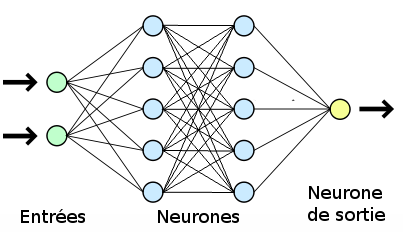
\includegraphics[width=13cm, height=7cm]{ANNsimple2.png}
\captionof{figure}{Réseau de neurones artificiel simple \cite{photANN}}
\end{center}
Ce qui vient d'être présenté est suffisant pour avoir une idée globale de ce qu'est réellement un réseau de neurones artificiel. Néanmoins, nous pousserons plus loin pour toucher le plus vite possible aux modèles qui nous intéressent dans ce travail.
\subsection{Les réseaux de neurones récurrents (\textit{RNN})}
$ _{} $ $ _{} $ $ _{} $ $ _{} $ $ _{} $Un \textit{RNN}(\textit{Recurrent Neural Network}) est un type de réseaux de neurones conçu en principe pour traiter les données séquentielles, comme les données textuelles,...\\
La principale différence structurelle entre les \textit{ANN simples} et les \textit{RNN} est l'existence des connexions de récurrence dans ces derniers. Il s'agit des boucles permettant la prise en compte des sorties passées dans le traitement final des données \cite{geron2020deep}.\\
Pour l'illustrer, rien de mieux qu'une image représentant la structure fonctionnelle des réseaux de neurones récurrents :\newpage
\begin{center}
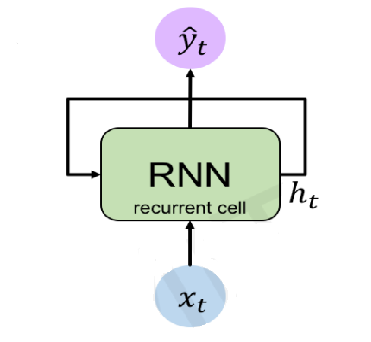
\includegraphics[height=4cm]{RnnsMIT2.png}
\captionof{figure}{Illustration de ce qu'est un RNN \cite{MITphot}}\label{IllustRNN}
\end{center}
Où $ x_{t} $, $ h_{t} $ et $ \hat{y}_{t} $ (à nommer juste $ y_{t} $) représentent respectivement les entrées, les états internes qui en résultent et les sorties (c'est-à-dire $ x $, $ h $ et $ y $ à chaque pas temporel $ t $).\\
Pour une meilleure compréhension, une présentation formelle serait plus commode :\\
Soient $ W_{x} $ la matrice des poids associée au vecteur d'entrée $ x $, $ W_{y} $ une matrice associée au vecteur de sortie $ y $ et $ W_{h} $ celle associée au vecteur représentant les états cachés du réseau, avec $ b_{h} $ et $ b_{y} $ respectivement les vecteurs des biais des neurones pour l'état caché et pour la sortie. On aura alors \cite{ganegedara2018natural} :
\begin{eqnarray}\label{eqRNN}
\begin{cases}
h_{t} &= f_{act}\left( W_{x}x_{t}+W_{h}h_{t-1}+ b_{h} \right)\\
y_{t} &= g_{act}\left( W_{y}h_{t} + b_{y} \right)
\end{cases}
\end{eqnarray}
On voit très bien que la sortie du système dépend non seulement de l'entrée, mais aussi de l'état du système ($ h $).\\
Les fonctions d'activation $ f_{act} $ et $ g_{act} $ qui sont mentionnées dans les équations \ref{eqRNN} représentent respectivement la \textit{tangente hyperbolique} $ tanh $ et la fonction dite $ softmax $ \cite{ganegedara2018natural}.

L'entraînement des réseaux de neurones récurrents se fait de la même façon que pour les réseaux de neurones simples (avec uniquement une différence due au fait que pour le \textit{RNN} on prend en compte le temps). On n'entrera pas dans le détail, vu que ce n'est pas exactement le sujet du travail mais, pour entamer la partie qui suit, il nous faut préciser que, comme pour les réseaux de neurones simples, l'entraînement exige d'appliquer une fonction de différentiation sur l'erreur produite par le système. Il s'agit de la fonction gradient. Mais, comme ici le gradient tient compte des grandeurs précédentes dans le temps, il y a un certain nombre de termes multiplicatifs qui peuvent amener le modèle à ne jamais converger ou au contraire, à la saturation. C'est le problème classique d'é\-va\-noui\-sse\-ment (disparition) des gradients ou d'explosion des gradients \cite{ganegedara2018natural}.\\
En réponse au problème de disparition des gradients, les cellules \textbf{\textit{LSTM}} (\textit{Long Short-Term Memory}) sont utilisées en lieu et place des cellules \textit{RNN} normales.
\subsubsection{Les cellules LSTM}
$ _{} $ $ _{} $ $ _{} $ $ _{} $ $ _{} $Les cellules \textit{LSTM} (pour \textit{Long Short-Term Memory}) sont utilisées en lieu et place des cellules \textit{RNN classiques} (dites \textit{vanilla}) pour permettre au réseau de traiter des séquences de plus en plus longues sans perte rapide d'information \cite{geron2020deep}. Pour cela, des éléments de contrôle de la mémoire de la cellule sont ajoutés. Pour illustrer nos propos, voici une image qui nous permettra de différencier une cellule RNN classique d'une cellule \textit{LSTM} :
\begin{center}
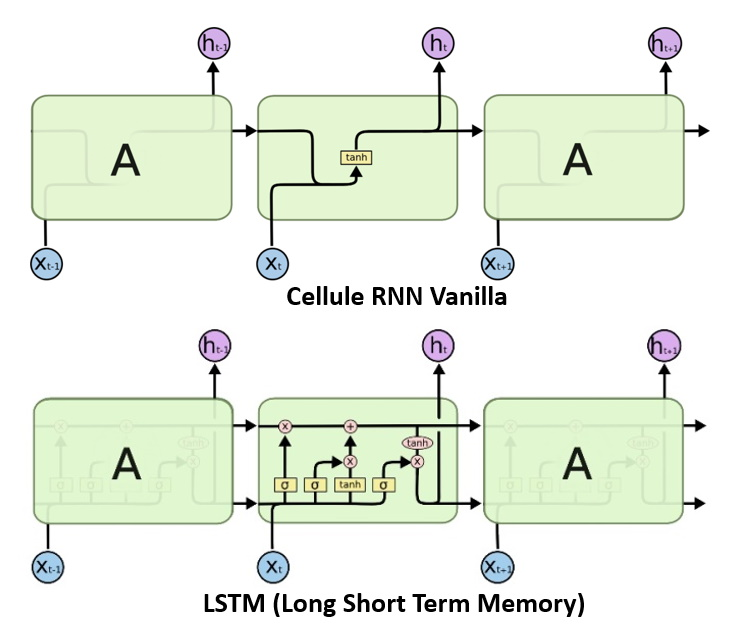
\includegraphics[height=10cm]{DiffRNN-LSTM.png}
\captionof{figure}{Comparaison entre cellules RNN classique et LSTM \cite{rnns}}
\end{center}
Présentée comme cela, la cellule \textit{LSTM} semble superflue mais si on présentait les équations associées à un réseau fait de ces cellules, on se rendra compte que c'est plutôt intuitif. Pour aborder les équations associées, considérons l'image suivante :\newpage
\begin{center}
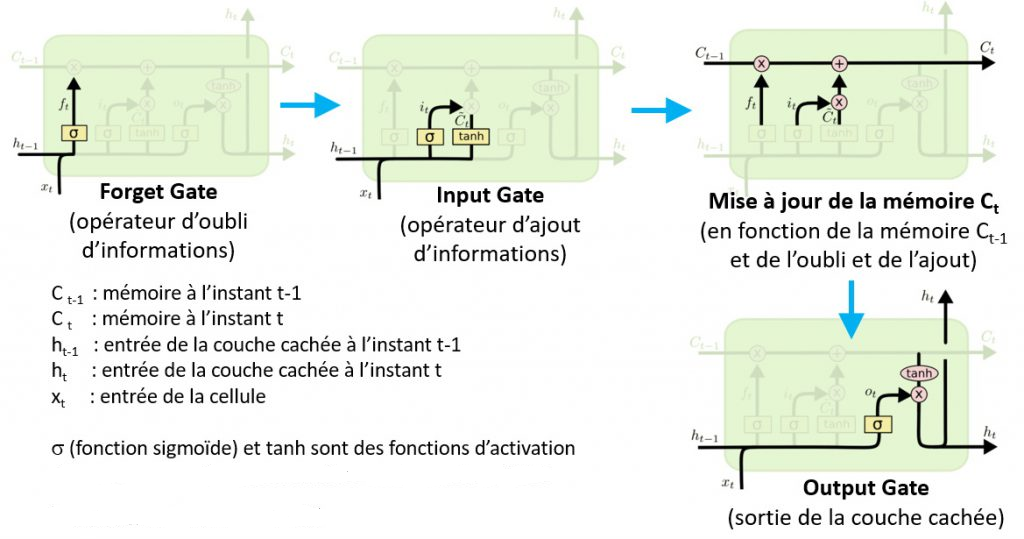
\includegraphics[width=16cm]{EqnLSTM.png}
\captionof{figure}{Vue fonctionnelle d'une cellule LSTM \cite{rnns}}
\end{center}
Une cellule \textit{LSTM} se comprend en la considérant comme constituée d'un ensemble de portes avec des fonctions bien particulières. Il s'agit d'une \textbf{porte d'entrée}, une \textbf{porte d'oubli} et une \textbf{porte de sortie}.\\
Il est évident que, pour chacune de ces portes que nous nommerons, à un instant $ t $ donné respectivement par $ I_{t} $, $ F_{t} $ et $ O_{t} $, le système doit apprendre ses paramètres en fonction de l'entrée et de l'état interne. Mais on doit aussi remarquer que, l'état est défini par deux paramètres au lieu d'un seul comme pour les RNN simples. Il s'agit, à un instant $ t $ donné, de $ h_{t} $ (considéré comme état à court terme) et de $ c_{t} $ (qui est un état à long terme mais dont le contenu est contrôlé, au vu de l'architecture de la cellule).\\
De ce que nous venons de dire, nous pouvons conclure que $ F_{t} $, $ I_{t} $ et $ O_{t} $ sont des fonctions de $ X_{t} $ et de $ h_{t-1} $ \textbf{aux poids près}. On sait aussi que, si on veut une mémoire à long terme contrôlée, la valeur finale de $ c_{t} $ doit être mise à jour en repérant ce qui doit être oublié parmi les éléments qui étaient précédemment dans la mémoire, pour y ajouter ensuite ce qui est sélectionné comme pertinent à l'entrée. Cela revient à utiliser $ F_{t} $ et $ I_{t} $ comme des portes de contrôle (ou de sélection). Et de cela on peut conclure que c'est plus intéressant d'avoir $ F_{t} $ et $ I_{t} $ qui prennent des valeurs entre $ 0 $ et $ 1 $ (pour modéliser la sélection) et $ c_{t} $ devra dépendre de ces deux éléments, avec aussi l'état précédent de la mémoire à long terme.\\
Il est aussi vraisemblable que, l'état à court terme doit provenir de la mémoire à long terme (ça correspondra à une sélection de ce qui doit être pris en compte directement dans la mémoire à long terme). Cet état $ h_{t} $ doit par conséquent dépendre de $ c_{t} $ (il faut néanmoins noter qu'une autre approche serait possible ici, mais celle-ci est déjà pertinente).\\
Finalement, on sait que la sortie finale doit nécessairement dépendre de l'état interne de la cellule. Il va ici s'agir de $ h_{t} $ vu que la cellule est développée par analogie avec le processus de mémorisation des systèmes naturels (mémoire à court terme correspondant à la mémoire de travail).

De ce qu'on vient de dire on peut tirer que, fondamentalement on doit avoir :
\begin{eqnarray}
\begin{cases}
F_{t} &= \mathcal{F}(X_{t},h_{t-1})\\
I_{t} &= \mathcal{G}(X_{t},h_{t-1})\\
O_{t} &= \mathcal{J}(X_{t},h_{t-1})\\
c_{t} &= \mathcal{K}(c_{t-1},X_{t},h_{t-1})\\
h_{t} &= \mathcal{L}(c_{t})\\
y_{t} &= \mathcal{M}(h_{t})
\end{cases}
\end{eqnarray}
Avec $ \mathcal{F}, \mathcal{G}, \mathcal{J}, \mathcal{K}, \mathcal{L}, \mathcal{M} $ des fonctions dépendant des coefficients considérés (poids et/ou éléments de sélection qui sont les diverses portes définies).\\
Une implémentation classique de ce raisonnement se présente comme suit \cite{geron2020deep,ganegedara2018natural} :
\begin{eqnarray}
\begin{cases}
F_{t} &= \sigma\left( W_{fx}X_{t}+W_{fh}h_{t-1}+b_{f} \right)\\
I_{t} &= \sigma\left( W_{ix}X_{t}+W_{fi}h_{t-1}+b_{i} \right)\\
O_{t} &= \sigma\left( W_{ox}X_{t}+W_{oh}h_{t-1}+b_{o} \right)\\
c_{t} &= F_{t}\circ c_{t-1} + I_{t}\circ \tanh\left( W_{cx}X_{t}+W_{ch}h_{t-1}+b_{c} \right)\\
h_{t} &= O_{t}\circ \tanh(c_{t})\\
y_{t} &= W_{yh}h_{t}+b_{y}
\end{cases}
\end{eqnarray}
Il faut remarquer qu'on a utilisé la fonction sigmoïde $ \sigma $ pour restreindre les valeurs des sélecteurs (portes) entre $ 0 $ et $ 1 $, puis on a utilisé le \textit{produit de Hadamard} (produit terme à terme des matrices) pour réaliser effectivement la sélection grâce aux portes, en diminuant les termes dont les valeurs correspondantes des portes sont proches de $ 0 $ et en essayant de conserver ceux dont les valeurs correspondantes des portes sont proches de $ 1 $.\\
Cette implémentation peut être modifiée, surtout en ce qui concerne les fonctions d'ac\-ti\-va\-tion utilisées ($ \sigma $ et $ \tanh $), et en particulier la fonction d'activation de finalisation $ \tanh $ ici, mais c'est l'une des plus optimales.

Le seul problème qui demeure est que le nombre de termes à apprendre est très grand. Cela a fait à ce qu'on puisse essayer de le diminuer en implémentant le \textit{\textbf{GRU}} (\textit{Gated Recurrent Unit}) poussant un peu plus loin l'abstraction des portes pour diminuer le nombre de paramètres.
\subsubsection{Les cellules GRU}
$ _{} $ $ _{} $ $ _{} $ $ _{} $ $ _{} $Les cellules \textit{GRU} (\textit{Gated Recurrent Unit}) sont une autre implémentation des cellules des réseaux de neurones récurrents comme les \textit{LSTM} à la différence près que, bien que partant de la même idée fondamentale évoquée précédemment, les \textit{GRU} apparaissent comme une simplification des \textit{LSTM}.\\
Elles possèdent néanmoins des performances comparables en ce qui concerne la prédiction des séries temporelles,... Les simplifications sont réalisées au niveau des états cachés et des portes. On conserve un seul état caché $ h $ (quitte à le contrôler à l'interne pour implémenter la mémorisation à long terme et à court terme). Et pour les portes, on fusionne les portes de sélection des entrées avec celle des éléments à oublier (donc les portes $ I $ et $ F $) pour former une porte dite de mise à jour (porte qui sera appelée \textit{update} ou $ U $). La porte de sélection des éléments de sortie quant à elle, est transformée en porte de réinitialisation.

Ces deux portes (de mise à jour et de réinitialisation) sont en fait implémentées de façon identique que celles des cellules \textit{LSTM}. La particularité des \textit{GRU} se situe prin\-ci\-pa\-le\-ment au niveau de la gestion de la mémoire (l'implémentation du processus de mémorisation) car, ayant supprimé la distinction long-terme/court-terme, il fallait bien trouver un mé\-ca\-ni\-sme devant permettre de bien gérer les deux aspects de la mémoire avec un seul état interne conservé.\\
C'est ainsi que, la porte de mise à jour (porte $ U $) est introduite dans le calcul de l'état $ h $ pour assurer la sélection du type de mise à jour à effectuer. Il s'agit de faire en sorte que, selon l'état interne et l'entrée, tout l'état interne précédent soit considéré  mais que certains éléments soient complètement modifiés, selon le besoin, et d'autres presque conservés.

Ainsi donc, $ h $ devient une combinaison d'éléments provenant de l'état interne précédent avec ceux provenant des nouveaux calculs effectués par la cellule (en fonction de l'entrée et de l'état interne précédent). Le comportement est alors le suivant :\\
Quand le vecteur de mise à jour a un terme proche de $ 1 $, cet état interne est presque conservé. Par conséquent, sa mise à jour est presque ignorée. Quand c'est plutôt $ 0 $, l'état interne précédent est presque ignorée et une mise à jour complète de cet état est effectuée. La formulation mathématique permet de mieux en saisir le fonctionnement \cite{geron2020deep,ganegedara2018natural} :
\begin{eqnarray}\label{EqnGRU}
\begin{cases}
U_{t} &= \sigma\left( W_{ux}X_{t}+W_{uh}h_{t-1}+b_{u} \right)\\
R_{t} &= \sigma\left( W_{rx}X_{t}+W_{ri}h_{t-1}+b_{r} \right)\\
h_{t} &= U_{t}\circ h_{t-1} + \left( 1-U_{t}\right)\circ \tanh\left( W_{hx}X_{t}+W_{hr}\left(R_{t} h_{t-1}\right) +b_{c} \right)\\
y_{t} &= W_{yh}h_{t}+b_{y}
\end{cases}
\end{eqnarray}
Et pour illustration, on peut considérer l'image suivante :
\begin{center}
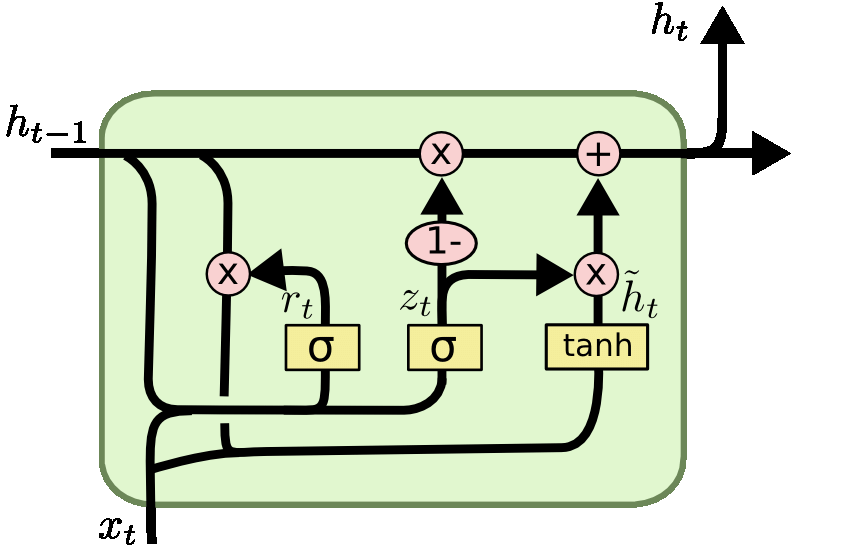
\includegraphics[scale=0.3]{Gated-Recurrent-Unit-GRU.png}
\captionof{figure}{Cellule GRU \cite{rnns}}\label{IllustGRU}
\end{center}
Il faut noter que sur cette image (figure \ref{IllustGRU}), l'implémentation de la mise à jour est l'inverse de celle que nous avons décrit par les équations \ref{EqnGRU}. C'est-à-dire que les termes $ U_{t} $ et $ \left( 1-U_{t}\right) $ sont permutés. Mais aussi, ici $ Z_{t} $ représente $ U_{t} $.\\

Ces modèles fonctionnent très bien et certaines implémentations permettent d'améliorer encore leurs performances. Ils sont néanmoins lents à entraîner, surtout à cause de l'aspect séquentiel. Parmi les techniques d'amélioration des performances, une peut être considérée car elle a un rapport direct avec notre travail. Il s'agit des \textbf{mécanismes d'attention} \cite{bahdanau2014neural}.\\
\subsection{Mécanismes d'attention}\label{AttentionEtseq2seq}
$ _{} $ $ _{} $ $ _{} $ $ _{} $ $ _{} $Les mécanismes d'attention sont en bref des techniques permettant de lutter contre la perte de mémoire qu'on constate par exemple dans les cellules récurrentes ci-haut décrites, en se focalisant sur des éléments les plus importants à chaque traitement. Le travail consiste donc à repérer, pour chaque entrée, les éléments sur lesquels se focaliser. C'est là qu'interviennent donc ces mécanismes.\\
L'une des implémentations les plus commodes est l'\textbf{attention globale} \cite{luong2015effective}.\\
Pour l'expliquer, nous allons considérer une architecture jusque là passée sous silence, mais qui permet aux modèles introduits là haut de s'utiliser efficacement pour les tâches courantes du \textit{NLP} en particulier. Il s'agit des modèles dits \textit{encodeur-décodeur}.\\
En effet, lorsqu'on a un modèle à séquence fonctionnel, les objectifs peuvent être multiples. On peut vouloir :
\begin{itemize}
\item[1°)] fournir une série d'éléments en entrée et ressortir une autre série (utile pour la prédiction de la valeur des actions par exemple,... );
\item[2°)] fournir un série en entrée mais faire ressortir un seul élément ou vecteur (utile pour la classification des textes, l'analyse des sentiments,...);
\item[3°)] fournir un vecteur plusieurs fois en entrée et produire une série (pour la génération des légendes pour des images par exemple,...);
\item[4°)] on peut aussi avoir un réseau série-vers-vecteur, appelé encodeur, suivi d'un réseau 
vecteur-vers-série, appelé décodeur (très utile pour la traduction et la synthèse au\-to\-ma\-ti\-que par exemple,...). Il s'agit du modèle \textbf{encodeur-décodeur}.
\end{itemize}
Une illustration par image sera suffisante :
\begin{center}
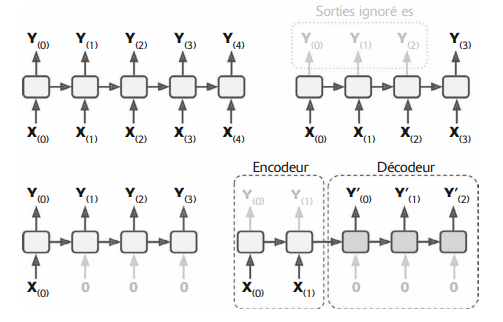
\includegraphics[scale=1]{IllustENC-DEC.PNG}
\captionof{figure}[Présentation des modèles encodeur-décodeur \cite{geron2020deep}]{Réseaux série-vers-série (en haut à gauche), série-vers-vecteur (en haut à droite), vecteur-vers-série (en bas à gauche) et encodeur-décodeur (en bas à droite) \cite{geron2020deep}}. \label{FigureSeq2Seq}
\end{center}
L'élément (le vecteur d'état) passé entre l'encodeur et le décodeur est dit \textbf{vecteur de contexte}. Il représente en quelques sortes un condensé des informations passés à l'entrée de l'encodeur. Toutefois, plus la séquence d'entrée est longue, plus le risque que la mémoire de certaines séquences puisse  s'étioler devient grand. Ainsi, si par exemple on est entrain de vouloir traduire une longue phrase, on peut finir par transmettre un vecteur de contexte qui a perdu toute information sur les premiers éléments de la séquence passée en entrée. C'est pour cela qu'au lieu de passer un vecteur de contexte général, les mé\-ca\-nis\-mes d'attention permettraient ici de ne se focaliser que sur certaines informations lors du traitement d'un élément particulier de la séquence (en ayant évidemment passé tous les états internes passés au décodeur). Pour le réaliser concrètement, le mécanisme d'attention global consiste à formater le vecteur de contexte en fonction des éléments de l'encodeur à prendre en compte lors du traitement par le décodeur.

Considérons que $ \Omega $, dont les termes sont représentés par $ w_{ij} $, est la matrice des poids d'attention normalisés par une fonction \textit{softmax} pour chaque ligne. Et que $ \Pi $, dont les termes sont représentés par $ \alpha_{ij} $, est la matrice des poids d'attention générée par le mé\-ca\-nis\-mes avant normalisation.Si les éléments $ c_{i} $ représentent à chaque fois le vecteur contexte final à l'étape $ i $ de décodage et les $ h_{j} $ sont les vecteurs d'état interne de l'encodeur, l'attention globale revient à réaliser la manipulation suivante, pour formater le vecteur de contexte à prendre en compte pour l'élément en cours de traitement \cite{luong2015effective} :
\begin{eqnarray}\label{EqnGlobAtt}
\begin{cases}
w_{ij} &= softmax(\alpha_{ij}) = \frac{e^{\alpha_{ij}}}{\sum_{k}e^{\alpha_{ik}}}\\
c_{i} &= \sum_{j}w_{ij}h_{j}
\end{cases}
\end{eqnarray}

La dernière relation du système \ref{EqnGlobAtt} revient à réaliser une somme pondérée des vecteurs d'état internes passés de l'encodeur, selon l'importance de chaque état pour le traitement en cours. De ces équations il faut aussi remarquer que la notation des sommations n'est pas rigoureuse. Cela est volontaire car c'est intuitif (on réalise des sommations sur tous les éléments).\\
Plusieurs techniques arrivant à réaliser l'attention existent. En général, comme on peut d'ailleurs le déduire des relations de l'attention globale, ces mé\-ca\-nis\-mes étaient utilisés dans le cadre des réseaux récurrents. Une question s'est toutefois naturellement posée : \textit{ne pourrait-on pas se passer des RNN pour mettre au point des réseaux complètement basés sur l'attention ?}. La réponse est oui, avec des ajustements adéquats pour résoudre les faiblesses des modèles classiques dans le traitement des données séquentielles. C'est cela qui a conduit aux modèles dits \textbf{\textit{transformers}} \cite{vaswani2017attention}.
\subsection{Les transformers}
Il s'agit des modèles dont l'architecture générique se présente comme suit :\newpage
\begin{center}
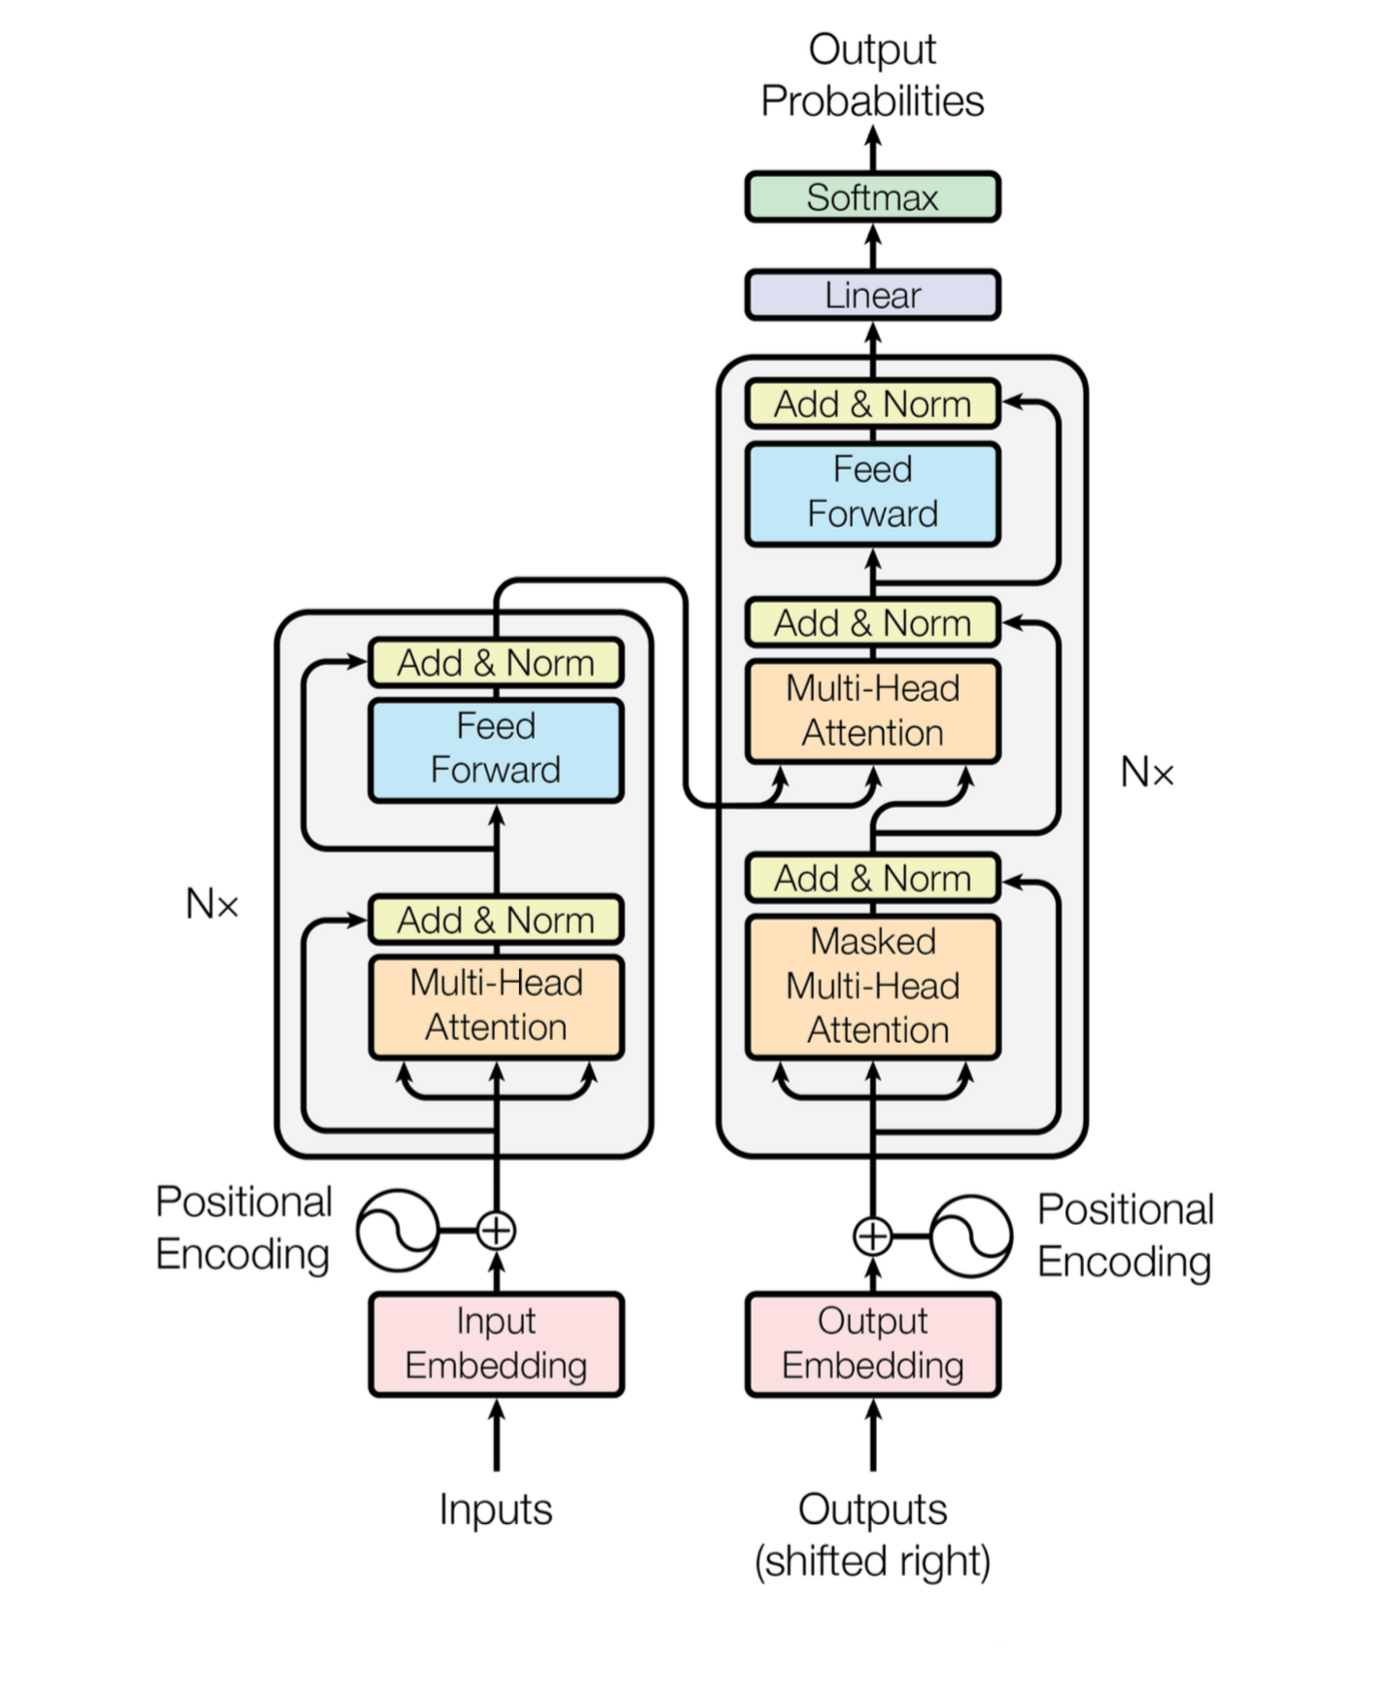
\includegraphics[scale=0.3]{TransformerVASWANI.PNG}
\captionof{figure}{Architecture générique des \textit{transformers} \cite{vaswani2017attention}}\label{ImgTransformerVASWANI}
\end{center}
Les \textit{transformers} sont des modèles du type \textit{encodeur-décodeur} comme on peut le constater sur la figure ci-dessus (bien que certaines implémentations n'en utilisent qu'une partie selon la tâche). Ils sont essentiellement basés sur les mécanismes d'attention, se passant de la récurrence \cite{geron2020deep,ganegedara2018natural}.\\
Nous donnerons une explication succincte de chacun des modules présents dans l'image \ref{ImgTransformerVASWANI}. En effet, présentons les modules selon l'ordre dans lequel les données traversent le modèle :
\begin{itemize}
\item[1°)] \textbf{Module d'embedding} : Nous savons que les données textuelles doivent être présentées au modèle sous forme numérique. Elles doivent donc être transformées avant de les passer aux parties suivantes. Néanmoins, vu que la représentation des entrées a un impact significatif sur les performances d'un modèle, cette représentation doit être bien choisie. Un choix intuitif, et qui s'avère être performant, est de tout faire pour que si deux termes ont des sens proches, ils aient aussi des représentations vectorielles proches. Cela est réalisé par différentes techniques que nous présenterons dans le chapitre suivant, mais c'est là le rôle de la couche d'enchâssement (\textit{embedding}).
\item[2°)] \textbf{L'encodage positionnel (\textit{positionnal encoding}}) : Ce module ajoute l'information sur la position relative de chacun des éléments placés en entrée par rapport aux autres. Cela pallie au problème de perte d'information sur la position des mots quand on utilise un réseau non séquentiel comme les réseaux récurrents. Donc, la position de chaque terme de la séquence placée en entrée est encodée dans un vecteur puis ajoutée à l'encodage global du terme. L'un des encodages les plus utilisés est celui basé sur les fonctions trigonométriques tel qu'introduit dans \cite{vaswani2017attention}.
\item[3°)] \textbf{Module d'auto-attention} :
La couche d'attention, présentée en première position dans la boîte de l'encodeur, est en fait une couche dite de \textit{self-attention} car elle opère sur la même séquence d'entrée. L'opération est réalisée pour permettre au modèle d'avoir une représentation de l'importance des termes dans la séquence d'entrée, les uns par rapport aux autres.\\
Pour illustration, considérons la phrase suivante : \textit{Walter est malade, il préfère se reposer}.\\
Dans cette phrase, l'un des constats qu'on peut faire est que, le nom "Walter" est beaucoup plus lié au pronom "il" qu'au verbe "préférer". C'est à l'établissement des tels liens dans les représentations que sert le module d'auto-attention ici présenté. Il est important que ce lien soit implicitement présent dans les représentations, pour que le traitement soit efficace comme on l'a mentionné lors de la présentation des mécanismes d'attention. Donc cette couche est en fait un prolongement de celle d'\textit{embedding}. Ici, le mécanisme d'attention utilisé est différent de celui qui a été présenté là-haut (attention globale). Il s'agit ici d'un mécanisme plutôt basé sur le produit scalaire mis à l'échelle (\textit{scaled dot-product}). En effet, très brièvement, l'idée du \textit{scaled dot-product attention} consiste à opérer une recherche des termes sur lesquels focaliser l'attention de la même façon qu'on réalise la recherche de la signification d'un mot dans un dictionnaire. Supposons qu'on veuille avoir la signification d'un mot dont on ne connaît pas l'orthographe exacte. Pour retrouver ce dernier dans un dictionnaire, il suffit de rechercher le mot qui ressemble le plus à l'orthographe que nous estimons être la plus vraisemblable. Mathématiquement, cette recherche de similitude correspond à un produit scalaire.\\
Similairement, le \textit{scaled dot-product} consiste à générer trois éléments qui sont \underline{la clé} ou \textit{key} $ k $, \underline{la valeur} ou \textit{value} $ v $ et \underline{la requête} ou \textit{query} $ q $. La \textit{requête} correspond au mot qu'on cherche (orthographié selon ce que nous pensons), la \textit{clé} correspond au mot présent dans le dictionnaire et la \textit{valeur} correspond à la signification associée. Si on supposait qu'il existe plusieurs termes du dictionnaire qui s'orthographient presque de la même façon que le mot qu'on cherche, on devra passer par une mesure de similarité avant de se décider sur le sens le plus probable. Cela correspond à réaliser le produit de tous les $ k $ par les $ q $ présents, puis à normaliser l'ensemble des résultats de manière à ce qu'ils représentent des mesures de probabilité, et finir par choisir le sens $ v $ le plus probable.\\
Pour aller plus vite, on implémente ce processus en considérant tous les $ k $, $ q $ et $ v $ au même moment de manière à réaliser le calcul une fois pour toutes. Cela revient à regrouper tous les $ k $, $ q $ et $ v $ dans des matrices $ K $, $ Q $ et $ V $. Ce qui donne la relation  qui définit l'attention par produit scalaire mis à l'échelle \cite{vaswani2017attention} :
\begin{eqnarray}\label{EqnScaledDotAtt}
Attention(Q,K,V) = softmax\left( \frac{Q\cdot K^{T}}{\sqrt{d_{k}}} \right)\cdot V
\end{eqnarray}
Dans cette relation, expression \ref{EqnScaledDotAtt}, le terme $ \sqrt{d_{k}} $ permet de mettre à l'échelle le résultat du produit scalaire de $ Q $ par $ K $, c'est-à-dire $ Q\cdot K^{T} $. Il faut noter que $ d_{k} $ est la dimension d'une clé, et que cette normalisation permet d'améliorer les performances du modèle mais elle n'est pas la seule envisageable.\\
Il est aussi important de remarquer que la couche d'attention utilise trois termes pour arriver à bout du problème. Ces trois termes sont obtenus par une transformation linéaire dont les poids sont appris à travers un réseau de neurones simple.\\
Il faut aussi noter que l'on utilise parallèlement plusieurs modules d'attention pour capture toutes les caractéristiques des séquences (on parle de \textit{multi-head attention}). Pour une plus ample illustration, voir la figure \ref{VueEclateeTrans}.
\item[4°)] \textbf{Le module \textit{feed-forward}} : Il s'agit en fait d'un réseau de neurones de propagation avant classique (réseau à couches ajoutées de façon séquentielle). Il permet de réaliser le traitement qui fait suite à l'attention.
\item[5°)] \textbf{Couche d'attention encodeur-décodeur} : Il s'agit de la couche qui reçoit les données en provenance de l'encodeur. Il s'agit ici d'une \textit{couche d'attention et non d'auto-attention} comme c'était le cas pour la première couche de l'encodeur. En effet, contrairement à la couche de \textit{self-attention}, pour laquelle tous les trois paramètres sont calculés à partir de la même séquence, la couche d'attention ici prend les clés $ K $ et valeurs $ V $ provenant de l'encodeur mais une requête $ Q $ provenant du décodeur.\\
Une autre couche \textit{feed-forward} suit celle-ci et a le même rôle que celle de l'encodeur.
\item[6°)] \textbf{Module d'attention masquée} : Il s'agit de la première couche du décodeur. C'est aussi un module de \textit{self-attention} auquel on ajoute le masquage. Ce module est dit masqué suite au fait que, comme le décodeur est un module de génération, on ne regarde que les termes précédemment générés, en masquant les termes qui seront probablement générés aux pas d'après. Cela est réalisé en rendant juste leurs probabilités nulles.
\item[7°)] \textbf{Module linéaire final} : Il s'agit d'un réseau de neurones classique pour réaliser la déduction finale, le tout étant passé à la fin à travers une opération \textbf{softmax} qui permet de transformer les résultats en probabilité d'éléments générés (cela permet de choisir le terme le plus vraisemblable à générer comme sortie).
\end{itemize}
Cette explication simplifiée se comprend mieux si on y joint la vue éclatée suivante :\newpage
\begin{center}
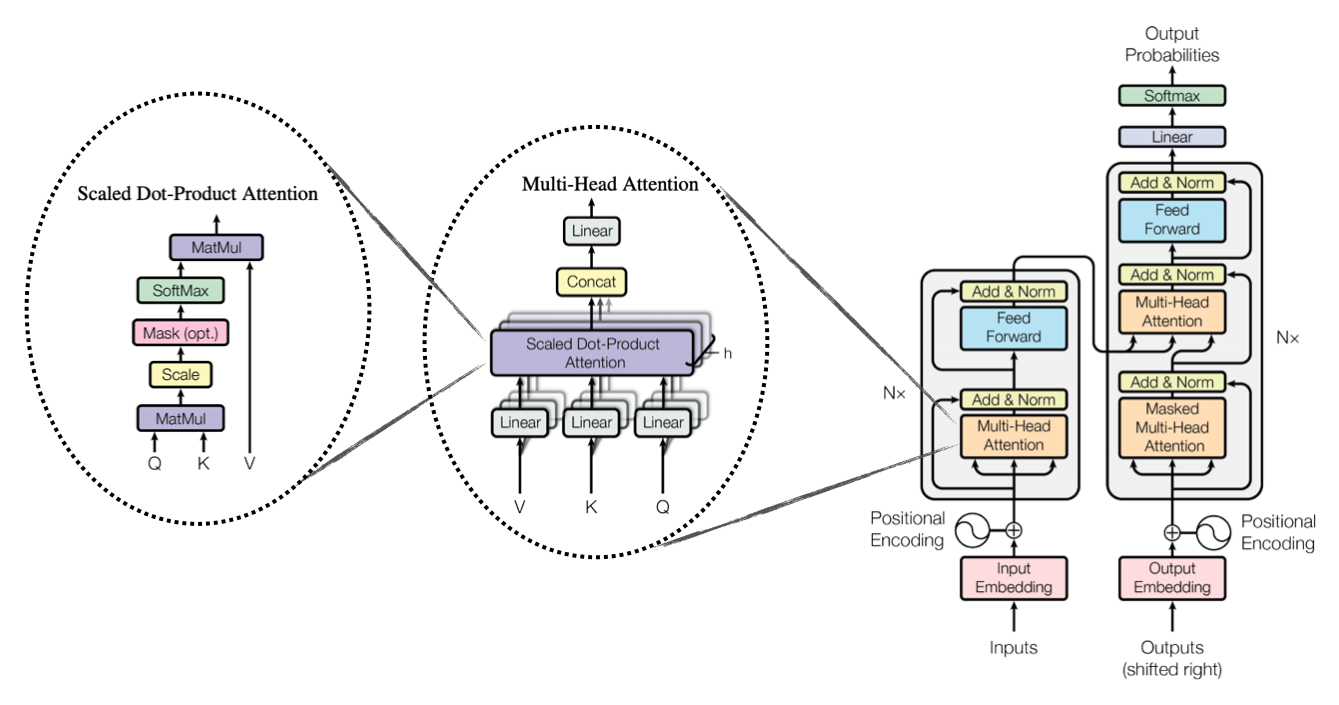
\includegraphics[width=16.5cm]{TransformerEclate2.PNG}
\captionof{figure}{Vue éclatée d'un transformer \cite{trans2020former}}\label{VueEclateeTrans}
\end{center}
Les \textit{transformers}, ici succinctement présentés, sont un modèle très adapté aux tâches de traitement automatique du langage naturel. C'est un modèle incontournable vu aussi que ses traitements peuvent être facilement parallélisés. Cela est rendu possible par le fait que l'architecture des \textit{transformers} est parallèle par essence. 
\section{Conclusion partielle}
$ _{} $ $ _{} $ $ _{} $ $ _{} $ $ _{} $Nous venons de réaliser une vue d'ensemble du domaine de traitement automatique du langage naturel, ainsi que diverses techniques couramment utilisées. Pour cela, nous avons tout d'abord justifié la préséance des modèles basés sur le \textit{deep learning} pour diverses tâches du NLP.\\
Ensuite, nous avons évoqué les technique de pré-traitement des textes, souvent in\-con\-tour\-na\-bles, comme la réduction des séquences en leurs tokens constitutifs, la suppression des mots fréquents mais n'apportant pas assez d'informations et la réduction des mots en leurs racines respectives. Nous y avons aussi joint quelques techniques utiles à la compréhension du langage humain comme le \textit{POS tagging} et la reconnaissance d'entités nommées. Ce qui précède nous a finalement conduit à présenter les modèles courants du NLP basés sur les RNNs et, nous avons terminé par la présentation de l'architecture \textit{transformer}, modèle que nous utiliserons pour ce travail (les précisions sur les modèles particuliers de \textit{transformer} à utiliser seront données au chapitre suivant).

Les transformers constituent un type de modèle qui s'avère être le plus adapté (pour le moment) au résumé automatique des textes et, dans le chapitre suivant, nous commencerons par présenter les diverses spécificités du résumé automatique comme tâche du NLP, pour finir par présenter l'architecture globale du système que nous comptons élaborer.
\chapter{ÉTUDE THÉORIQUE DU FILTRAGE DU SON}
\section{Introduction partielle}
$ _{} $ $ _{} $ $ _{} $ $ _{} $ $ _{} $Le résumé automatique étant le sujet principal de ce mémoire, dans cette partie nous le présentons alors en détail en tant que discipline et tâche du \textit{NLP}. Nous allons ici présenter les théories sur la synthèse automatique des textes, en classifiant les diverses méthodes utilisées, afin de pouvoir situer notre système dans l'ensemble des travaux jusque-là menés sur ce sujet.

Ensuite, nous présenterons les diverses approches utilisées pour le résumé automatique, sans oublier d'approfondir notre présentation des modèles de type \textit{transformer} adaptés à cette tâche, pour finalement mentionner le modèle que nous estimons le plus adapté concernant l'approche basée sur le \textit{deep-learning} pour la synthèse automatique.\\
Enfin, nous allons réaliser une conception rapide mais suffisante de l'architecture globale de notre système, que nous appellerons \textbf{\textit{Mon Résumeur}}, tout en précisant le rôle et le fonctionnement de chaque partie.
\section{Présentation et définitions}
$ _{} $ $ _{} $ $ _{} $ $ _{} $ $ _{} $Selon Le Petit Robert, résumer c'est reprendre en plus court un discours, le présenter brièvement en conservant l'essentiel. En d'autres termes, c'est l'abréger, l'écourter, le réduire.
De même, en tant qu'exercice intellectuel, le résumé, consiste à réduire un texte tout en lui restant fidèle. Il exige donc de restituer les idées en un nombre déterminé de mots,  en évitant au mieux de recopier le texte à résumer. Il faut alors composer un texte plus court qui contienne l'essentiel du message initial \cite{fasoEduc}.\\
De cela on tire que le résumé devient automatique s'il est généré par un logiciel ou un système informatique.\\
$ _{} $ $ _{} $ $ _{} $ $ _{} $ $ _{} $Cette définition est en fait correcte bien qu'elle ne soit pas assez précise pour notre contexte. Il nous faut une définition assez générale et précise, embrassant au mieux l'aspect automatique, ou mieux, l'aspect informatique, qui nous intéresse dans ce mémoire.\\
Une définition assez valable est celle de Torres-Moreno Juan-Manuel qui dit qu'\textit{un résumé automatique est un texte généré par un logiciel, cohérent et contenant une partie im\-por\-tan\-te des informations pertinentes de la source, et dont le taux de compression est inférieur au tiers de la taille du(des) document(s) source(s)} \cite{torres2014automatic}.\\
$ _{} $ $ _{} $ $ _{} $ $ _{} $ $ _{} $L'introduction du taux de compression dans la définition n'est pas anodine car, on s'est très vite rendu compte que la performance d'un système de résumé automatique dépendait fortement du taux de compression. En effet, les études de \cite{Lin1999TrainingAS} montrent que les meilleures performances des systèmes de résumé automatique sont généralement atteintes pour des taux de compression compris entre $ 15 $ et $ 30\% $ \cite{torres2014automatic}.\\
$ _{} $ $ _{} $ $ _{} $ $ _{} $ $ _{} $Nous allons adopter, dans ce travail, la définition de Torres-Moreno Juan-Manuel ci-haut présentée.\\

Toutefois, on ne doit pas manquer de signaler que la génération automatique des résumés est un problème complexe en soi, tout comme l'évaluation des résultats. Le résumé est en effet une tâche cognitive requérant la compréhension du texte considéré et, les humains n'étant pas toujours bons dans les tâches de synthèse, le manque d'étalon explique qu'il y ait également une difficulté d'automatisation du processus.
\section{Catégorisation des résumés}
$ _{} $ $ _{} $ $ _{} $ $ _{} $ $ _{} $Les résumés peuvent être classifiés selon différents critères tels que leur fonction, le nombre de documents source, le genre de document, le type de résumé, le type de résumeur, le contexte,...\\
Parcourons de manière succincte ces différents critères de classification \cite{MaaliMnasri,maaloul:tel-00756111,mani2001automatic,Nenkova,moens2001automatic,torres2014automatic}
:
\subsection{Selon la fonction}
$ _{} $ $ _{} $ $ _{} $ $ _{} $ $ _{} $Selon leur fonction, on classifie les résumés en deux groupes qui sont le \textit{résumé indicatif} et le \textit{résumé informatif}.
\subsubsection{Résumé indicatif}
$ _{} $ $ _{} $ $ _{} $ $ _{} $ $ _{} $Tel une table des matières, un résumé indicatif renseigne le lecteur sur les thèmes abordés dans un document. Il liste donc les sujets les plus importants évoqués par le texte. Certains systèmes de résumé guidé génèrent un résumé indicatif du texte comme étape initiale, l'utilisateur choisit alors parmi les sujets proposés par le résumé ceux qui l'intéressent et le système produit enfin un résumé informatif du texte, guidé par la requête de l'utilisateur. La requête dans ce cas est l'ensemble des sujets sélectionnés à partir du résumé indicatif.
\subsubsection{Résumé informatif}
$ _{} $ $ _{} $ $ _{} $ $ _{} $ $ _{} $Il s'agit d'un modèle rétréci du texte d'origine, relatant le plus largement possible les informations contenues dans celui-ci. Ce type de résumé répond souvent à une attente en résumant de plus le contenu. La problématique ici est donc double : comprendre ce qui n'est pas information dans un texte et connaître le besoin de l'utilisateur final.\\
Néanmoins, si on n'a pas de requête spécifique de la part de l'utilisateur, le résumé informatif est réalisé en veillant à ce que l'ensemble des principaux sujets du texte d'origine soit rapporté. Ainsi, les sujets principaux qui sont rappelés dans le résumé sont répartis de manière fidèle par rapport à l'organisation initiale afin de donner un juste aperçu du texte source.\newpage
\subsection{Selon le nombre de documents sources}
$ _{} $ $ _{} $ $ _{} $ $ _{} $ $ _{} $Selon le nombre de documents sources on a les résumés mono-document et multi-document.
\subsubsection{Résumé mono-document}
$ _{} $ $ _{} $ $ _{} $ $ _{} $ $ _{} $Il consiste à résumer un document isolé. Le corpus de documents source est donc ici constitué d'un seul et unique document. 
\subsubsection{Résumé multi-documents}
$ _{} $ $ _{} $ $ _{} $ $ _{} $ $ _{} $Il s'agit d'un résumé de plusieurs documents (un groupe de documents), très souvent liés thé\-ma\-ti\-que\-ment, en faisant attention à ne pas insérer des informations déjà évoquées.
\subsection{Selon le genre des documents}
\subsubsection{Résumé des documents journalistiques}
$ _{} $ $ _{} $ $ _{} $ $ _{} $ $ _{} $Il s'agit de résumer les documents du type article de presse (sachant qu'ils ont une structure particulière). En effet, on sait par exemple que dans le domaine journalistique, les informations les plus importantes sont souvent mentionnées au début du texte.\cite{MaaliMnasri}
\subsubsection{Résumé des documents spécialisés}
$ _{} $ $ _{} $ $ _{} $ $ _{} $ $ _{} $Il s'agit de résumer des documents en provenance d'un domaine précis (géologie, médecine, mathématique,...), fortement spécialisé.
\subsubsection{Résumé des documents littéraires}
$ _{} $ $ _{} $ $ _{} $ $ _{} $ $ _{} $C'est le résumé de documents du type narratif, des textes littéraires, des textes ar\-gu\-men\-ta\-tifs, ...
\subsubsection{Résumé des documents encyclopédiques}
$ _{} $ $ _{} $ $ _{} $ $ _{} $ $ _{} $Ici il s'agit de résumer des documents de type encyclopédique (en général multi-thématiques de toute évidence) à l'exemple de Wikipédia...
\subsection{Selon le type de sortie (résumé obtenu)}
$ _{} $ $ _{} $ $ _{} $ $ _{} $ $ _{} $Cette classification est très importante et très utilisée. Il s'agit des :
\subsubsection{Résumé extractif (\textit{extractive summarization})}
$ _{} $ $ _{} $ $ _{} $ $ _{} $ $ _{} $Le résumé extrait est formé de segments de texte extraits du(des) document(s) source(s). Ces segments peuvent être des phrases, des propositions ou n'importe quelle unité textuelle présent dans le(s) document(s) à résumer. Le problème consiste donc à repérer les segments de texte qui semblent être les plus pertinents pour faire partie du résumé final. Les éléments obtenus à la fin sont donc explicitement présents dans le(s) document(s) source(s).
\subsubsection{Résumé abstractif (\textit{abstractive summarization})}
$ _{} $ $ _{} $ $ _{} $ $ _{} $ $ _{} $Les méthodes de résumé abstractives imitent, jusqu'à un certain degré, le processus naturel accompli par l'homme pour résumer un document. Par conséquent, elles produisent des résumés plus similaires aux résumés manuels (humains). Ce processus peut être décrit par deux étapes majeures : la compréhension du texte source et la génération du résumé. La première étape vise à analyser sé\-man\-ti\-que\-ment le contenu du texte et à identifier les parties à exprimer dans le résumé. C'est en quelques sortes une tâche d'extraction d'information liée au domaine abordé ou de regroupement des phrases du texte source. Vient ensuite la génération du texte.\\
Bref, on produit un résumé rapportant le contenu du(des) texte(s) source(s) en utilisant un vocabulaire souvent différent et plus concis.\\

Il existe aussi des résumés dits \textit{semi-extractifs}, et même aussi des résumés dits \textit{par compression} \cite{torres2014automatic} mais nous estimons inutile de les décrire ici étant donné que la distinction abstractif-extractif suffit pour notre contexte.
\subsection{Selon le type de résumeur}
$ _{} $ $ _{} $ $ _{} $ $ _{} $ $ _{} $Le résumeur est le système qui réalise le résumé. Il peut s'agir d'une entité naturelle (un humain) ou artificielle (un logiciel). On a donc es\-sen\-tiel\-lement les deux cas suivants :
\subsubsection{Résumé humain (manuel)}
$ _{} $ $ _{} $ $ _{} $ $ _{} $ $ _{} $Il s'agit d'un résumé réalisé par un humain. Il peut être fait par l'auteur même du document (on parle souvent de \textit{résumé d'auteur}), par un expert du domaine traité (on parle souvent de \textit{résumé d'expert}) ou par un professionnel de résumé (on parle de \textit{résumé professionnel}).
\subsubsection{Résumé automatique}
$ _{} $ $ _{} $ $ _{} $ $ _{} $ $ _{} $Il s'agit, comme on l'a maintes fois mentionné, d'un résumé fait par un système informatique.
\subsection{Selon le contexte}
\subsubsection{Résumé générique}
$ _{} $ $ _{} $ $ _{} $ $ _{} $ $ _{} $Ici on résume le document sans prendre en compte les besoins d'information de l'utilisateur. On produit juste un résumé complet et le plus mieux fait possible.
\subsubsection{Résumé guidé}
$ _{} $ $ _{} $ $ _{} $ $ _{} $ $ _{} $Pour ces types de résumé, l'utilisateur commande la génération du résumé en précisant les types d'information dont il a besoin.
\subsubsection{Résumé mis à jour}
$ _{} $ $ _{} $ $ _{} $ $ _{} $ $ _{} $Il s'agit d'un résumé de type dynamique par essence. Ici, un ensemble de documents sources est résumé en veillant minutieusement à ce que le document dont le résumé est ajouté à la suite d'un précédent résumé ne puisse pas créer une répétition d'information. Il y a donc un contrôle de nouveauté.\newpage
\subsection{Selon le destinataire du résumé}
$ _{} $ $ _{} $ $ _{} $ $ _{} $ $ _{} $On peut aussi classifier un résumé selon le public auquel il est destiné.
\subsubsection{Résumé sans profil}
$ _{} $ $ _{} $ $ _{} $ $ _{} $ $ _{} $Il s'agit d'un résumé qui ne tient pas compte d'un quelconque profil utilisateur. Le résumé est donc généré sans tenir compte de la personnalité des utilisateurs.
\subsubsection{Résumé avec profil}
$ _{} $ $ _{} $ $ _{} $ $ _{} $ $ _{} $Il s'agit d'un résumé dont l'un des éléments guides (requête) est le profil des individus auxquels le résumé est destiné.\\

\textbf{En ce qui concerne notre système, nous implémenterons à la fois un résumeur abstractif et un résumeur extractif et ce sera mono-document. En plus de cela, le résumé ne sera pas guidé, il s'agira de produire des résumés génériques, pour des documents de type littéraire (documents du type narratif, des textes littéraires, des textes argumentatifs,...).}
\section{Approches de résumé automatique}
$ _{} $ $ _{} $ $ _{} $ $ _{} $ $ _{} $Nous allons présenter ici diverses approches algorithmiques pour résumer les documents textuels. Les approches seront abordées en supposant que les résumés sont prin\-ci\-pa\-le\-ment classés en \textit{abstractif} et \textit{extractif}.
\subsection{Techniques intuitives de résumé \cite{MaaliMnasri}}
$ _{} $ $ _{} $ $ _{} $ $ _{} $ $ _{} $Avec des \textbf{critères centrés sur le contenu des textes}, il existe un grand nombre d'al\-go\-ri\-thmes assez triviaux de résumé, qui sont basés entre autres sur :
\begin{itemize}
\item[•] La fréquence d'occurrence des mots et
\item[•] L'annotation en rôle sémantique.
\end{itemize}
Ces critères mettent l'accent sur le contenu du texte et le message qu'il communique.
\subsubsection{Fréquence d'occurrence des mots}
$ _{} $ $ _{} $ $ _{} $ $ _{} $ $ _{} $L'idée majeure des techniques qui utilisent ce critère consiste à considérer que les mots les plus fréquents sont les plus liés au sujet principal du texte à résumer. Cette approche assez simpliste mais fonctionnelle fut introduite en $ 1958 $ par \textbf{Luhn} \cite{Luhn58}, une première tentative de résumé automatique.\\
On affecte des scores aux phrases présentes dans le texte, en additionnant chaque fois les poids des mots les constituant (on attribue ce poids en fonction de la fréquence d'apparition du mot considéré dans le texte entier). Et, à la fin, le résumé est constitué avec les phrases extraites du texte source, et dont le score dépasse un certain seuil dépendant de la taille maximale imposée pour le résumé. Le tout est finalement réarrangé selon l'ordre d'apparition (des phrases sélectionnées) dans le texte d'origine.
\subsubsection{L'annotation en rôle sémantique}
$ _{} $ $ _{} $ $ _{} $ $ _{} $ $ _{} $Ici, l'idée est simple. En utilisant des techniques de repérage d'entités nommées (voir le chapitre précédent), on identifie les entités présentes dans le document. Après cela, l'entité la plus fréquente est identifiée et considérée comme entité principale. Par la suite, les phrases contenant cette entité sont sélectionnées. Enfin, seules les phrases où l'entité principale possède un rôle sémantique fondamental (non auxiliaire) sont gardées pour le résumé.\\
L'un des moyens les plus simples pour repérer les entités nommées est de passer par l'apprentissage profond comme on l'a précédemment mentionné.\\

Il existe tout de même des \textbf{techniques qui ne se fient qu'à la forme et à la structure du texte}, sans en considérer le contenu. L'intuition derrière cette approche est basée sur le constat que dans un texte, les éléments ne sont pas présentés de façon arbitraire. De manière usuelle, les techniques utilisées se basent sur :
\begin{itemize}
\item[•] La position des phrases;
\item[•] La similarité avec le titre 
\item[•] La longueur des phrases ou sinon,
\item[•] Les mots indices (\textit{cue word})
\end{itemize}
\subsubsection{La position des phrases}
$ _{} $ $ _{} $ $ _{} $ $ _{} $ $ _{} $Cette approche est à appliquer en fonction de la nature du document et de son genre. Pour certains types de documents (documents journalistiques par exemple), les phrases se trouvant au début sont généralement plus informatives et décrivent le sujet principal du document. De plus, les phrases situées au début de chaque paragraphe tendent à apporter plus d'informations pertinentes. Le résumé des articles scientifiques par contre, peut essentiellement se former en se basant sur les contenus des parties \textbf{résumé} et \textbf{introduction} (sous l'hypothèse que ces dernières parties sont bien faites). En revanche, dans le cas des revues intégratives (critique et comparaison des études), les phrases les mieux notées sont celles des parties \textbf{résultats et discussion} et \textbf{conclusion}.\\
Ces exemples suffisent pour illustrer dans quelle mesure cette approche peut s'appliquer.
\subsubsection{La similarité avec le titre}
$ _{} $ $ _{} $ $ _{} $ $ _{} $ $ _{} $Cette approche part du principe selon lequel un bon titre doit informer de manière brève du contenu principal du texte qu'il encadre. Cela permet alors de fixer comme mesure de pertinence des phrases, leur similarité avec les titres. Toute la problématique se réduit donc à la construction d'algorithmes capables de capturer efficacement la similarité.
\subsubsection{La longueur des phrases}
$ _{} $ $ _{} $ $ _{} $ $ _{} $ $ _{} $L'approche consistant à se baser sur la longueur des phrases est assez naïve mais fonctionnelle.\\
En effet, la longueur moyenne d'une phrase dans un texte dépend de son genre. Gé\-né\-ra\-le\-ment, les phrases très courtes sont considérées comme peu informatives alors que les phrases très longues sont présumées favoriser la redondance. Cette caractéristique est exploitée en fixant un intervalle de longueur (entre 15 et 30 mots). Une phrase ayant une longueur en dehors de cet intervalle est pénalisée \cite{Schiffman2002}.
\subsubsection{Les mots indices}
$ _{} $ $ _{} $ $ _{} $ $ _{} $ $ _{} $Ici, on considère une liste de mots, constituée manuellement, et qui a comme rôle de permettre de se décider si une phrase doit être prise dans le résumé ou rejetée, selon qu'elle contient ou non un(des) mot(s) de la liste qualifié(s) inhibiteur(s) ou valorisant(s). Comme exemple des mots ou groupes de mots inhibiteurs on trouve : \textit{par exemple}, \textit{ac\-ces\-soi\-re\-ment}, ... Et pour les mots valorisants on peut citer : \textit{notez bien}, ...\\
Nous devons quand même préciser encore une fois que tout dépend de celui qui écrit la liste.\\ 

Les méthodes que nous venons de présenter sont assez intuitives mais constituent la base des processus de synthèse. En effet, synthétiser un texte revient au fond à implémenter un certain nombre de règles, dont font parties évidemment celles que nous venons de mentionner. Néanmoins, ce que nous venons de présenter est décrit en se basant sur le concept de résumé extractif. Nous devons toutefois signaler que les résumés abstractifs se basent au fond sur les mêmes principes, soit en partant des résumés extractifs pour ensuite réaliser des paraphrases, insérer des connecteurs appropriés et éliminer les ré\-fé\-ren\-ces anaphoriques dans les résumés, soit en implémentant indirectement toutes ces techniques à travers un modèle d'\textit{apprentissage automatique} ou un \textit{modèle basé sur les graphes} capables de capturer d'un seul coup tous ces aspects (ou une grande partie d'entre-eux). Les techniques intuitives ci-haut présentées ne sont pas les seules. Il en existe également d'autres, basées essentiellement sur les théories linguistiques. Entre autres \textbf{les méthodes d'analyse du discours} (par exemple la \textit{\textbf{RST}} \cite{maaloul:tel-00756111} ou \textit{Rhetorical Structure Theory})...

\subsection{Algorithmes classiques de résumé automatique}
$ _{} $ $ _{} $ $ _{} $ $ _{} $ $ _{} $Comme nous venons de l'introduire dans la section précédente, le résumé automatique est abordé es\-sen\-tiel\-le\-ment selon deux approches qui sont \cite{maaloul:tel-00756111} :
\begin{itemize}
\item[1°)] Les \textit{approches numériques}, fondées sur les techniques à base des scores (poids), et
\item[2°)] Les \textit{approches symboliques} fondées sur les techniques purement linguistiques, basées en premier sur une étude sémantique.
\end{itemize}
Il faut noter qu'on peut considérer aussi des \textit{approches basées sur la théorie des graphes} comme intégrant les idées de ces deux approches de façon implicite, tout comme celles basées sur l'\textit{apprentissage automatique}. Mais, dans tous les cas, une vue sur quelques heuristiques (méthodes basées sur le bon sens) est toujours à considérer (surtout en amont et en aval du processus de synthèse).\\
Ici, nous allons présenter les approches essentiellement numériques (on va y inclure celles basées sur l'apprentissage automatique et celles basées sur la théorie des graphes).

\subsubsection{Algorithme de Luhn \cite{Luhn58}}
$ _{} $ $ _{} $ $ _{} $ $ _{} $ $ _{} $Il s'agit d'une méthode semi-heuristique pour la synthèse des documents. C'est la plus ancienne méthode de résumé automatique (au sens moderne du terme).\\
Cette approche n'est pas considérée comme très bien formalisée. Elle exécute impli\-ci\-te\-ment l'approche du \textit{Tf-Idf} que nous allons décrire dans la sous-section qui suit celle-ci (sous-section \ref{SousSecTFIDF}).\\
La sélection (des mots ici) se fait en considérant les hypothèses qui suivent :
\begin{itemize}
\item[-] la synthèse consiste à supprimer certains mots pour n'en conserver que les plus importants;
\item[-] les mots se trouvant au début sont probablement importants;
\item[-] les autres mots utiles respectent une certaine distribution. La figure \ref{Luhn58Phot} montre, selon \textit{Luhn}, comment choisir ces mots importants (partie hachurée de la courbe).\newpage
\begin{center}
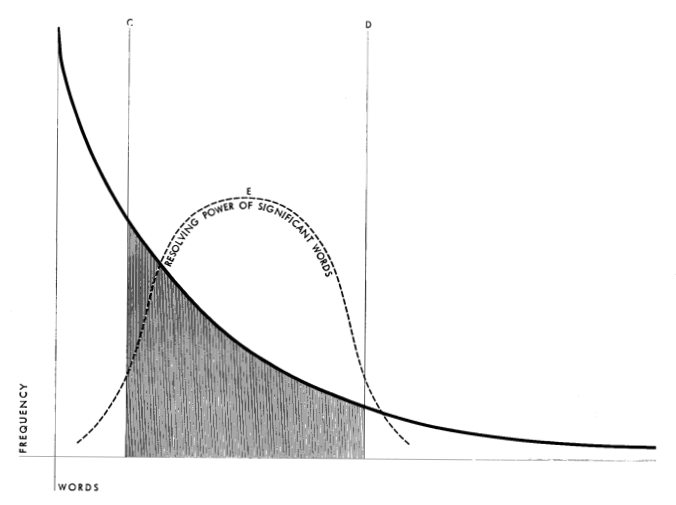
\includegraphics[scale=0.8]{Luhn58Phot.png}
\captionof{figure}{Diagramme des fréquences des mots et le choix de Luhn \cite{Luhn58}}\label{Luhn58Phot}
\end{center}
\end{itemize}
Cette approche, comme on l'a mentionné au début, est assez moins précise et empirique, mais elle sous-tend les idées fondamentales appliquées plus tard.

\subsubsection{Algorithme TF-IDF}\label{SousSecTFIDF}
$ _{} $ $ _{} $ $ _{} $ $ _{} $ $ _{} $Le \textit{\textbf{tf-idf}} (\textit{time-frequency inverse document frequency}) est une approche essentiellement utilisée pour le résumé extractif. Il s'agit d'une correction de l'approche naïve consistant à poser que plus un mot est répété dans un corpus de texte, plus il y est important.\\

Soit donc un corpus constitué de $ D $ documents et $ N_{j} $ le nombre total de mots (termes) présents dans un document $ j $ donné du corpus. Nommons $ Freq(i,j) $ le nombre de fois qu'un terme $ i $ apparaît dans le document $ j $.\\
On définit classiquement la fréquence d'apparition par :
\begin{eqnarray}
TF(i,j) = \frac{Freq(i,j)}{N_{j}}
\end{eqnarray}
L'approche qui se base naïvement sur la fréquence d'apparition des mots dans les textes pour juger de leur importance relative, accorde à chaque mot un poids égal à $ TF(i,j) $.\\
La grande faiblesse de cette approche est d'inclure ainsi des termes sans grande pertinence in\-for\-ma\-tion\-ne\-lle comme des prépositions, des articles,... très présents au sein des documents.\\

Pour corriger cette faiblesse, on pose l'hypothèse que les termes importants apparaissent plusieurs fois dans un document (ou juste dans peu de documents du corpus) et non pas dans plusieurs documents, puisque dans le cas où c'est dans plusieurs documents, il est souvent question des éléments communs du langage, sans grande utilité informationnelle. Ceci constitue en fait \textit{la loi de Zipt} \cite{vzivzka2019text} et c'est le fondement de l'approche du \textit{tf-idf}.\\

A cet effet, on définit $ DF_{i} $ comme étant le nombre de documents dans le corpus, qui contiennent le terme numéro $ i $. Cela permet d'affecter alors le poids selon la formule \cite{berry2010text} :
\begin{eqnarray}\label{Tf-Idf-Formula}
TFIDF(i,j) = \log\left(1+TF(i,j)\right)\cdot\log\left(\frac{D}{DF_{i}}\right)
\end{eqnarray}
Dans l'expression \ref{Tf-Idf-Formula}, en supposant que $ N $ est le dictionnaire des termes présents dans l'ensemble des documents et $ D $ le nombre de documents du corpus, il faut noter que :\\
$ i \in \left\lbrace 1,...,N\right\rbrace $ et $ j \in \left\lbrace 1,...,D\right\rbrace $.\\

D'où finalement, le poids d'un terme $ i $ dans un document $ j $ est donné par :
\begin{eqnarray}
w_{ij} = TFIDF(i,j)
\end{eqnarray}
Pour notre cas, l'application de cette approche consiste à décomposer un long texte en ses phrases et de considérer que chacune de ces phrases est un document et que le texte entier constitue le corpus.\\

Plusieurs définitions des éléments $ TF(ij) $ et $ IDF_{i} $ formant l'expression \ref{Tf-Idf-Formula} sont toutefois possibles selon les besoins en terme  de performance.\\
Mais, dans l'ensemble, l'idée de base demeure la même car il ne s'agit en général que de changement des types de normalisation \cite{vzivzka2019text}.\\

L'application de cette méthode pour le résumé consiste fi\-na\-le\-ment à calculer le poids de chaque phrase en additionnant les poids des termes la constituant, puis à normaliser le résultat en fonction de la taille de la phrase considérée. Après tout, on définit un seuil qui permet de soutirer les phrases selon leur pertinence ainsi évaluée (en considérant évidemment plus pertinente une phrase dont le résultat de la sommation des poids est élevé).
\subsubsection{Algorithme TextRank}
\textit{TextRank} est un algorithme de résumé extractif, basé sur la théorie des graphes et qui s'inspire de l'algorithme \textit{PageRank} de Google \cite{brin1998anatomy,benincasa2006page}.\\
A la base, on considère un ensemble de $ N $ phrases donné, et on calcule les coefficients de liaison de chaque phrase aux $ N-1 $ autres. A la fin, on peut obtenir une matrice $ M $ de taille $ N\times N $ dont chaque terme $ M_{ij} $ représente le degré de liaison entre la phrase numéro $ i $ et la numéro $ j $. Il s'agit en fait d'une \textit{matrice d'adjacence} dans laquelle on pose au préalable que $ M_{ii} = 0 \mbox{, pour tout } i $ (c'est la même idée pour l'algorithme \textit{PageRank} étant donné qu'il est logique de considérer qu'une page ne peut s'auto-référencer).\\

Soit donc $ i \in \left\lbrace 1,..., N \right\rbrace $. Appelons $ Phr_{i} $ la phrase numéro $ i $ du corpus. Cela veut dire qu'on peut écrire :
\begin{eqnarray}
Liaison \mbox{ } Phr_{i}\leftrightsquigarrow Phr_{j} = M_{ij} = M_{ji}
\end{eqnarray}
Les valeurs de $ M_{ij} $ sont calculées au choix, selon le programmeur. Ce dernier implémente en effet une mesure de similarité selon sa définition de la liaison entre phrases et les besoins en performance.\\
C'est ainsi qu'on peut utiliser par exemple une mesure de similarité classique nommée \textit{similarité cosinus} en la basant par exemple sur $ TFIDF $ \cite{COSINindurkhya2010handbook}.\\
Pour représenter les mots à comparer, on utilise les méthodes classiques de vectorisation des mots (\textit{word embedding}). Nous esquisserons ces méthodes dans les sections qui vont suivre, parlant du \textit{word embedding} ( \ref{SectionSeq2Seq} ).\\

Le rang des phrases sont alors calculés de manière itérative en s'inspirant de la formule \cite{mihalcea2004textrank} :
\begin{eqnarray}\label{TextR-Formula}
TextRank\left(Phr_{i}\right) = (1-K)+K\cdot \sum\limits_{\underset{j \neq i}{j=1}}^N \left[TextRank(Phr_{j})\right]\cdot M_{ij}
\end{eqnarray}
Dans cette formule, $ K $ est une constante comprise entre $ 0 $ et $ 1 $.\\
Initialement, on prend en général une valeur identique de $ TextRank(Phr_{i}) $ pour toutes les phrases (souvent $ TextRank(Phr_{i})=1 $), mais la valeur initiale prise n'affecte pas les valeurs finales, mais elle affecte le temps de convergence \cite{mihalcea2004textrank}.\\

La formule \ref{TextR-Formula} n'est pas arbitraire, elle est d'ailleurs triviale si on s'inspire de l'algorithme de \textit{PagePank} la plus simple. Pour cet algorithme (\textit{PageRank}), on avait pris à l'origine $ K=0.85 $ \cite{brin1998anatomy}.\\
\paragraph{\underline{Justification de la formule}}
Le principe de \textit{PageRank} consiste à se dire que, si une page $ Pag_{i} $ contient $ N_{i} $ références vers d'autres pages, la probabilité qu'on aille vers l'une de ces pages référencées est de $ \frac{1}{N_{i}} $ (avec l'hypothèse que les références ne sont pas répétées et que la distribution de leur importance est uniforme). On sait tout de même que plus une page est référencée, plus on doit lui donner de l'importance.\\
Si alors on pose que l'importance de la page $ Pag_{i} $ est connue, le calcul de l'importance d'une page $ Pag_{j} $ vers laquelle elle pointe se calculera logiquement par :
\begin{eqnarray}\label{PageRankBEGIN}
Importance(Pag_{j}) = \sum_{i} Importance(Pag_{i})\cdot \frac{1}{N_{i}}
\end{eqnarray}
Avec $ i $ appartenant à l'ensemble des pages qui mentionnent la page $ Pag_{j} $ en leur sein.\\
Malheureusement, pour les phrases non référencées (pages dites isolées), on trouve une importance nulle. Pour lutter contre cela, la formule \ref{PageRankBEGIN} est un peu modifiée en y introduisant adéquatement une constante non nulle $ K $.\\
Ce qui donne l'expression \cite{brin1998anatomy} :
\begin{eqnarray}\label{PageRank}
Importance(Pag_{j}) =(1-K) + K\cdot\sum_{i} Importance(Pag_{i})\cdot \frac{1}{N_{i}}
\end{eqnarray}
On voit alors qu'il s'agit belle et bien de la formule utilisée pour \textit{TextRank} (formule \ref{TextR-Formula}).\\

Après initialisation des rangs de chaque phrase du texte ( les $ TextRank(Phr_{i}) $) et après calcul de la matrice d'adjacence $ M $. On applique la formule \ref{TextR-Formula} itérativement et à la convergence, on choisit les phrases qui vont former le résumé selon leur importance ( valeurs des $ TextRank(Phr_{i}) \mbox{ pour toute valeur de } i $).\\
A la fin, les phrases sélectionnées sont réarrangées pour former un résumé extrait plus ou moins cohérent.\\

Il existe également un algorithme nommé \textit{\textbf{LexRank}} \cite{erkan2004lexrank} qui est assez similaire à \textit{TextRank} ici décrit, à la différence près que :
\begin{itemize}
\item[-] Il prend essentiellement en compte les métriques de similarité robustes;
\item[-] Il considère la position et la longueur des phrases dans le calcul de leur pertinence;
\item[-] Il est optimisé pour le résumé multi-document.
\end{itemize}

Plusieurs autres algorithmes populaires existent, par exemple les algorithmes \textit{\textbf{LSA}} (\textit{Latent Semantic Analysis} ou Analyse Sémantique Latente) et \textit{\textbf{LDA}} (\textit{Latent Dirichlet Allocation} ou Allocation Latente de Dirichlet) \cite{berry2010text}.\\
Le premier, la \textit{LSA}, est un algorithme statistique, basé sur l'algorithme \textit{\textbf{SVD}} (\textit{Singular Value Decomposition} ou décomposition en valeurs singulières). Seulement, cette technique est très gourmande en ressources suite à la complexité de l'algorithme qui implémente le \textit{SVD}. Le second, la \textit{LDA}, basé sur la détection des thématiques, peut aussi être utilisé.\\

Toutefois, il faut remarquer que les algorithmes ici présentés sont essentiellement adaptés à la synthèse extractive. Même si ces traitements peuvent être mélangés avec les \textbf{techniques de résolution d'anaphores} et les \textbf{paraphrases} pour obtenir des synthèses qui tendent vers la synthèse abstractive, nous devons souligner que les techniques jusque là les plus performantes pour la synthèse abstractive sont essentiellement basées sur le \textit{deep learning} \cite{MaaliMnasri}. Le \textit{deep learning} peut également être utilisé pour la synthèse extractive, permettant ainsi la génération des synthèses extraites plus cohérentes (avec résolution d'anaphores). Ainsi donc, nous abordons les méthodes de \textit{deep learning} utilisées pour cet effet dans les parties qui suivent.
\section{Modèles Seq2Seq}\label{SectionSeq2Seq}
\subsection{Methodes du Word-Embedding}
$ _{} $ $ _{} $ $ _{} $ $ _{} $ $ _{} $Tout traitement commence par une représentation numérique des termes (des mots ici) pour qu'ils soient assimilables par le modèle. Une approche naïve consisterait à regrouper tous les mots de notre vocabulaire dans une liste (un dictionnaire) et de les représenter chacun par un nombre unique (un identifiant). Une autre approche, plus classique, consiste à représenter chaque mot par un vecteur de dimension égale à la taille du dictionnaire et dont tous les termes sont nuls, sauf à la position, dans le dictionnaire, du mot qu'on est entrain de vouloir représenter (on parle du \textit{one-hot encoding}).\\
$ _{} $ $ _{} $ $ _{} $ $ _{} $ $ _{} $Ces représentations, et toutes celles qui s'y apparentent, ont la grande faiblesse d'être peu  informatives (au point de vu sémantique). Étant artificiellement construites, sans tenir compte du sens des mots, ni de leur contexte, ces méthodes de représentation rendent la tâche de découverte des caractéristiques par les systèmes de \textit{machine learning} encore plus difficile. D'ailleurs, l'une des faiblesses de la seconde méthode décrite (le \textit{one-hot encoding}) est que les vecteurs sont creux (une majorité de valeurs nulles) et de dimension inutilement très grande. On pourrait directement songer à une représentation plus ju\-di\-cieu\-se pour éviter ces deux soucis, et qui consisterait à réaliser une représentation binaire des termes mais, le problème de la sémantique sera toujours là.\\
$ _{} $ $ _{} $ $ _{} $ $ _{} $ $ _{} $On recourt donc à des méthodes de représentation plus élaborées, partant du principe selon lequel le contexte d'un mot suffit pour en appréhender le sens. Ainsi, tout mot est représenté en réalisant une statistique (implicitement bien sûr) sur les divers mots qui l'accompagnent souvent, de telle sorte que les mots aux sens proches aient aussi des vecteurs très proches. Bref, on en arrive à réaliser la proposition : "Similarité sémantique implique similarité de représentation". Ce sont les méthodes classiques du \textit{word embedding} (ou plongement lexical). Il s'agit par exemple des méthodes comme le \textit{\textbf{Word2Vec}} \cite{WORD2VECmikolov2013efficient, WORD2VEC2mikolov2013distributed}, \textit{\textbf{Glove}} \cite{GLOVEpennington2014glove}, \textit{\textbf{fastText}} \cite{FASTtEXTbojanowski2017enriching}...\\

\subsection{Modèles séquence-à-séquence proprement dits}
$ _{} $ $ _{} $ $ _{} $ $ _{} $ $ _{} $S'agissant des modèles séquence-à-séquence (\textit{Seq2Seq}), ils ont été présentés dans la section \ref{AttentionEtseq2seq} (voir particulièrement la figure \ref{FigureSeq2Seq}). Il s'agit bel et bien des modèles adaptés aux tâches de synthèse, vu qu'en entrée on reçoit une séquence pour ressortir une autre séquence en sortie.\\
Comme nous l'avons déjà bien mentionné au précédent chapitre, nous n'allons parler que des modèles \textit{Seq2Seq} de type \textit{transformer} car actuellement, ils sont les plus adaptés à la tâche que nous voulons réaliser (celle de synthèse automatique). Les \textit{transformers} (voir la figure \ref{ImgTransformerVASWANI}) sont un modèle très avantageux car en fait, au-delà de leurs performances et autres avantages, ils facilitent encore plus la recherche en \textit{NLP} en rendant effectif le \textit{transfer learning} (apprentissage par transfert) dans ce domaine.\\

L'entraînement des \textit{transformers} est \textit{semi-supervisé}. Il se fait en deux crans (nous les décrirons dans le cadre du \textit{NLP}) :
\begin{itemize}
\item[1°)] \textit{\textbf{Pré-entraînement}} : il s'agit d'un \textit{apprentissage non supervisé}, qui consiste à donner au modèle une masse colossale de données textuelles, non étiquetées, pour qu'il développe une compréhension statistique du langage qu'on veut qu'il puisse assimiler. Au final, on obtient un modèle pré-entraîné.
\item[2°)] \textit{\textbf{Affinage de l'apprentissage}} (\textit{fine-tuning}) : Ça consiste à finaliser l'apprentissage du modèle pré-entraîné \textit{de manière supervisée} pour qu'il soit en mesure de réaliser une tâche donnée du \textit{NLP} (il s'agit du \textit{transfer learning} en fait). Cette spécialisation, requiert une très faible quantité de données car le modèle aura déjà une représentation assez bonne de la langue. Cela pallie à la fois au problème de manque des données labellisées en \textit{NLP} et de la consommation en terme de ressource énergétique des gros modèles lors de leur entraînement. 
\end{itemize}
Les méthodes de pré-entraînement sont très déterminantes pour les performances finales du modèle. Ce premier entraînement du modèle a pour rôle de l'amener à construire un \textit{\textbf{modèle de langage}} \cite{BART}.\\
Il existe ainsi plusieurs objectifs de de pré-entraînement (pour construire le modèle de langue). On peut par exemple entraîner le modèle à :
\begin{itemize}
\item[-] Prédire le mot suivant : donc, lors de cet entraînement non supervisé, on fournit chaque fois au modèle une séquence de mots en lui demandant de prédire le suivant. Il s'agit d'un objectif d'entraînement dit \textit{NSP} (\textit{Next Sentence Prediction}) visant à transformer implicitement le \textit{transformer} en un modèle de langue  \cite{BERT_devlin2018bert};
\item[-] Deviner le mot caché (masqué) : on fournit au modèle du texte dont certaines parties (mots ou suite de mots) sont cachées. L'objectif assigné au modèle est alors de retrouver les mots masqués. On parle du \textit{MML} (\textit{Masked Language Modelling}) \cite{BERT_devlin2018bert}.
\end{itemize}
Ainsi, au fur et à mesure, les paramètres du modèle s'affinent, le transformant en un modèle de langue performant. Mais, à part les deux que nous venons de mentionner, il existe d'autres \textit{objectifs de pré-entraînement} \cite{BART,PEGASUSzhang2020pegasus} selon les variantes de \textit{transformers} et les objectifs finaux de spécialisation du modèle.\\

Bien que la forme classique des \textit{transformers} est bel et bien celle de la figure \ref{ImgTransformerVASWANI}, il existe $ 3 $ types d'implémentation selon les types de tâche visées en dernier lieu :
\begin{itemize}
\item[1°)] Modèles à encodeur seul : on supprime la partie décodeur. Ces modèles sont très bons pour les tâches de compréhension du langage comme la classification par exemple.
\item[2°)] Modèles à décodeur seul : on supprime alors la partie décodeur du modèle. Ils sont bons pour les tâches de génération de texte.
\item[3°)] Modèles encodeur-décodeur : ou encore modèles \textit{seq2seq} proprement-dits. Ils sont bons pour les tâches demandant à la fois la compréhension et la génération des textes.
\end{itemize}
Pour illustrer ce fait, on va considérer donc $ 3 $ types de \textit{transformers} \cite{GRAAL_HF_tunstall2022natural, HF_wolf2020transformers} :
\begin{itemize}
\item[1°)] \textit{Like-BERT} : semblables au transformer dénommé \textit{BERT} (\textit{Bidirectional Encoder Re\-pre\-sen\-ta\-tions from Transformers}). Ce sont des modèles du type encodeur seul. Ils sont également bidirectionnels. Donc, les phrases sont lues dans les deux sens pour mieux saisir tout le contexte.
\item[2°)] \textit{Like-GPT} : donc semblables au \textit{transformer} dénommé \textit{GPT} (\textit{Generative Pre-trained Transformer}) qui n'ont que la partie décodeur et sont dits \textit{auto-regressifs} car, seules les parties précédant le mot en cours de traitement sont connues du modèle et il y a chaque fois réinjection des sorties à l'entrée.
\item[3°] \textit{Like-BART/T5} : semblables à \textit{BART} (\textit{Bidirectional and Auto-Regressive Transformers}) ou à  \textit{T5} (\textit{Text-To-Text Transfer Transformer}). C'est donc ceux du type encodeur-décodeur.
\end{itemize}
\paragraph{\underline{Modèles encodeurs (\textit{encoder-model})} :} Comme on l'a dit, pour ces modèles, on n'imp\-lé\-men\-te que la partie encodeur du \textit{transformer} d'origine (celui d'origine étant dans \cite{vaswani2017attention}). En plus de cela, ces modèles ont une couche d'attention bidirectionnelle et sont généralement appelés \textit{auto-encodeurs} (\textit{auto-encoding model}). Ces modèles sont principalement bons pour les tâches de \textit{NLU} (\textit{Natural Language Understanding}) comme la classification, le \textit{NER} (\textit{Name Entity Recognition}), l'\textit{extractive question-answering},...\\
Dans ce groupe, les modèles les plus connus sont :
\begin{itemize}
\item[•] ALBERT \cite{lan2019albert},
\item[•] BERT \cite{BERT_devlin2018bert},
\item[•] DistilBERT \cite{sanh2019distilbert},
\item[•] RoBERTA \cite{liu2019roberta},
\item[•] Etc.
\end{itemize}

\paragraph{\underline{Modèles décodeurs (\textit{decoder-models})} :}
Utilisent seulement la partie décodeur, sont auto-regressifs et par conséquent les têtes de \textit{self-attention} n'accèdent qu'aux mots précédant l'étape à laquelle elles sont (pas de regard dans le futur) comme on l'a déjà un peu mentionné. Ces modèles sont particulièrement bons pour les tâches liées fortement au \textit{NLG} (\textit{Natural Language Generation}).\\
Dans ce groupe, les modèles les plus connus sont :
\begin{itemize}
\item[•] Les GPT ($ 1 $, $ 2 $ et $ 3 $) \cite{GPT2_radford2019language},
\item[•] TransformerXL \cite{dai2019transformer},
\item[•] Etc.
\end{itemize}

\paragraph{\underline{Modèles encodeur-décodeur (\textit{sequence-to-sequence models})} :}
Ces modèles utilisent l'in\-té\-gra\-li\-té de l'architecture des \textit{transformers} et sont ainsi bons pour les tâches demandant à la fois du  \textit{NLU} et du \textit{NLG} comme la synthèse automatique abstractive, le \textit{generative question-answering} et la traduction automatique.\\
Ici nous pouvons particulièrement mentionner les modèles comme :
\begin{itemize}
\item[•] BART \cite{BART},
\item[•] mBART \cite{mBART_liu2020multilingual},
\item[•] BARThez \cite{eddine2020barthez},
\item[•] T5 \cite{T5-raffel2020exploring},
\item[•] mT5 \cite{mT5_xue2020mt5},
\item[•] PEGASUS \cite{PEGASUSzhang2020pegasus},
\item[•] Etc.
\end{itemize}

\subsection{Modèle BART pour la synthèse abstractive}\label{BARTmodel}
Le modèle \textit{BART} est comme une combinaison de \textit{BERT} \cite{BERT_devlin2018bert} et de \textit{GPT-2} \cite{GPT1_radford2018improving,GPT2_radford2019language} en terme d'architecture et d'objectif de pré-entraînement, avec quelques optimisations supplémentaires \cite{BART}.
Pour illustration, voici une image de comparaison :
\begin{center}
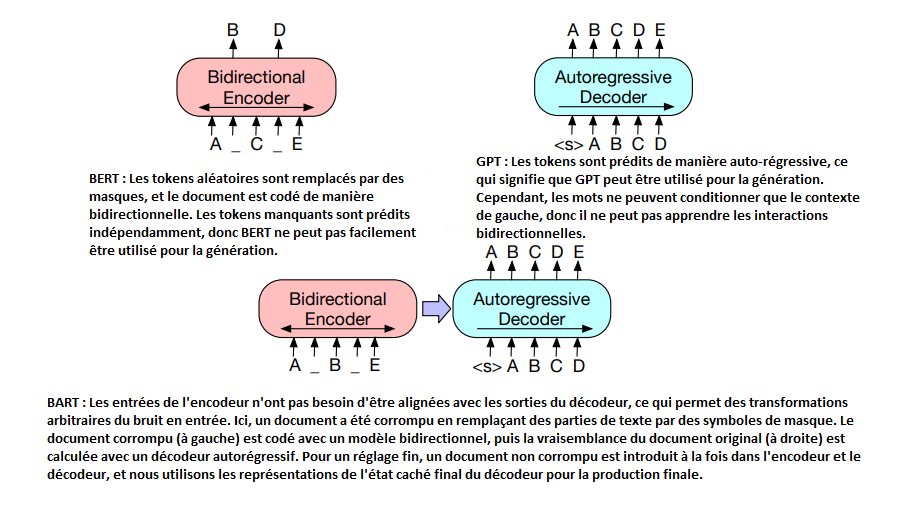
\includegraphics[width=15cm]{GPT_BERT_BART.png}
\captionof{figure}{Comparaison simplifiée entre BERT, GPT et BART \cite{BART}}\label{ComparisonBART}
\end{center}
$ _{ } $\\
L'image \ref{ComparisonBART} étant claire, nous pouvons illustrer les diverses corruptions que peuvent subir les données pour le pré-entraînement. L'image ci-dessous l'illustre :\newpage
\begin{center}
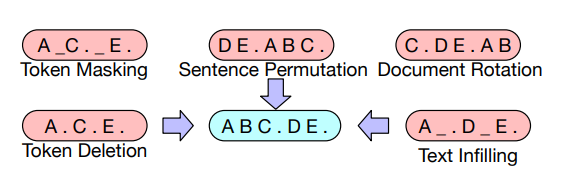
\includegraphics[scale=1]{TransForNOISING.png}
\captionof{figure}{Transformations de bruitage expérimentées pour BART \cite{BART}}
\end{center}
Le modèle \textit{BART} est bien adapté à la tâche de synthèse abstractive. C'est celui que nous allons utiliser (les modèles dérivés de \textit{BART} principalement) pour réaliser cette tâche dans notre système.
\subsubsection{Justification du choix de BART}
$ _{} $ $ _{} $ $ _{} $ $ _{} $ $ _{} $Le choix de \textit{BART} est dû au fait que c'est le modèle que nous avons trouvé réalisant un bon compromis poids-performances. Aussi, après quelques tests, ses résultats nous ont paru être plus intéressants. En outre, l'objectif d'entraînement utilisé pour \textit{BART} nous paraît assez général pour construire un modèle de langage performant. Nous justifierons plus précisément ce choix dans le chapitre qui suit, en présentant également quelques résultats des tests.
\section{Conception de l'architecture globale de \textit{Mon Résumeur}}
$ _{} $ $ _{} $ $ _{} $ $ _{} $ $ _{} $Il existe un large éventail des méthodes de développement des systèmes informatiques mais, en règle générale, toutes suivent les étapes suivantes \cite{CoursGenieLogiciel} :
\begin{itemize}
\item[1°)] Spécifications : on définit avec précision ce que fera le système (à quoi est-il destiné?);
\item[2°)] Conception et mise en oeuvre : on conçoit et on réalise le système;
\item[3°)] Validation : on teste le système pour voir s'il correspond aux objectifs précisés dans les spécifications;
\item[4°)] Évolution : ça correspond à tout ce qui vient après la livraison du produit (\textit{versionning}, maintenances,...).
\end{itemize}
Ici, on ne va pas utiliser une méthode de conception particulière. Pour pouvoir tout de même y aller méthodiquement, nous nous inspirerons de ces étapes classiquement suivies lors de la conception des systèmes informatiques.\\
Dans ce second chapitre, nous ne présenterons que les spécifications du système ainsi qu'une ébauche de conception avec une présentation de l'architecture globale. La suite sera traitée dans le chapitre suivant.
\subsection{Spécifications du système}
$ _{} $ $ _{} $ $ _{} $ $ _{} $ $ _{} $Le système devra pouvoir permettre de réaliser ce qui suit :
\begin{itemize}
\item[-] Synthétiser les textes qui lui sont fournis en entrée (saisis directement ou importés dans fichiers \textit{.pdf} non scannés, des fichiers \textit{.docx} et \textit{.txt});
\item[-] Servir les synthèses directement ou à travers un fichier \textit{.pdf} à télécharger;
\item[-] Obtenir des synthèses produites par plusieurs algorithmes et les évaluer;
\item[-] Stocker les couples document-synthèse;
\item[-] Permettre l'affinage d'un modèle de synthèse automatique (ici nous réaliserons le \textit{fine-tuning} du modèle \textit{mBART} ou du modèle \textit{mT5} selon celui qui se prêtera mieux à cet affinage).
\end{itemize}
C'est cela le minimum de besoins que le système devra être capable de combler.
\subsubsection{Exigences fonctionnelles}
Pour fonctionner, nous allons considérer que les fichiers chargés (pour en obtenir le résumé) seront au format \textit{pdf}, \textit{txt} ou \textit{docx} et qu'ils seront en français.
\subsubsection{Exigences non fonctionnelles}
Comme exigence non fonctionnelle, on doit noter qu'un processus d'authentification sera utile, songeant à une rentabilisation future du système.
\subsection{Présentation des éléments du système}
$ _{} $ $ _{} $ $ _{} $ $ _{} $ $ _{} $L'architecture globale de notre système est un trois-tiers classique. Elle se présentera comme sur la figure \ref{ArchiSysteme}:
\begin{center}
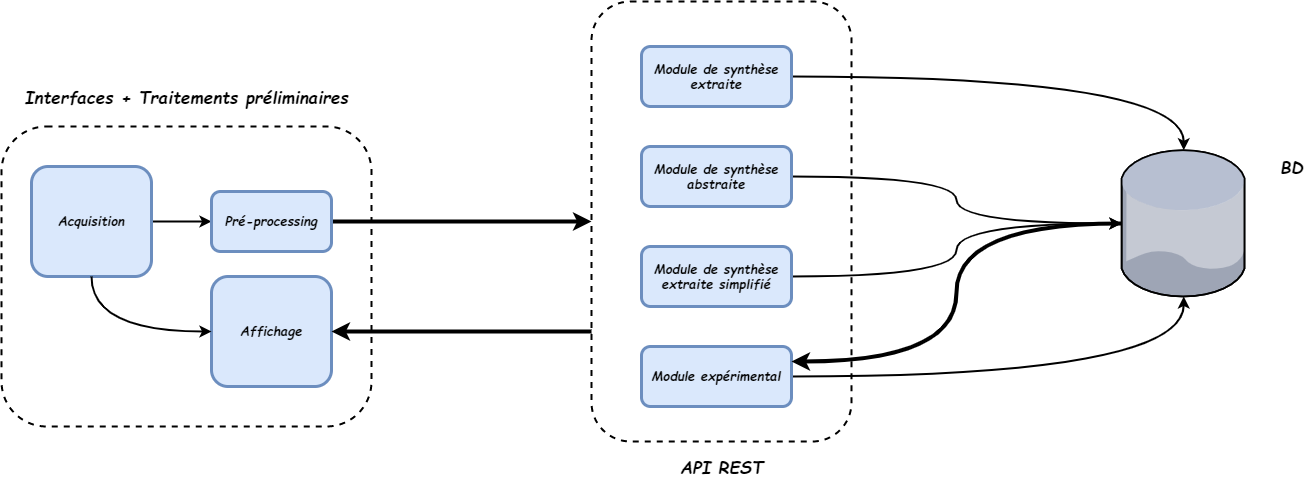
\includegraphics[width=16cm]{ArchiSysteme.png}
\captionof{figure}{Architecture globale de notre système}\label{ArchiSysteme}
\end{center}
La figure \ref{ArchiSysteme} présente l'architecture du système qui est une architecture $ 3-tiers $ classique. Il y a toutefois une partie qui n'est pas ici représentée car nous voulons nous donner une grande liberté de conception à son sujet. Il s'agit en fait de l'interface d'accès à l'\textit{API} (\textit{Application Programming Interface}), qui permettra aux développeurs de s'authentifier et générer éventuellement un \textit{token} à utiliser pour implémenter leurs propres interfaces devant permettre d'utiliser les services de cette \textit{API}. Il s'agit donc d'une \textit{API privée}.\\
Cette interface permettra aussi de voir toute la documentation de l'\textit{API} (pour les dé\-ve\-lop\-peurs) pour mieux utiliser ses services.

Quant au bloc interface que nous venons de présenter sur la figure \ref{ArchiSysteme}, c'est en nous mettant à la place d'un développeur lambda qui exploite les services de l'\textit{API}.\\
$ _{} $ $ _{} $ $ _{} $ $ _{} $ $ _{} $Notre \textit{API} quant à elle, est une \textit{API} \textit{REST} (\textit{REpresentationnal State Transfer}) qui aura $ 4 $ \textit{end-points} principaux dédiés à la synthèse automatique (selon les besoins d'imp\-lé\-men\-ta\-tion, on pourra en insérer d'autres mais qui ne concernerons probablement pas la synthèse).
\begin{itemize}
\item[•] \textit{Module de synthèse extraite} : ce module réalisera une synthèse en combinant divers résultats d'algorithmes de synthèse extraite. Nous prévoyons, dans un premier temps, ne l'utiliser que pour des petits documents (la taille optimale sera déterminée avec les expérimentations au chapitre suivant).
\item[•] \textit{Module de synthèse abstraite} : ce module donnera une synthèse abstraite en utilisant l'un des \textit{transformers} affinés pour la synthèse ou bien par le module qui sera en train d'être amélioré au cours de l'utilisation du système (on l'a nommé \textit{expérimental} sur les interfaces, voir la figure \ref{EbaucheInterface}). Comme les \textit{transformers} réalisent des synthèses de documents de taille généralement limitée à environ une page, nous mettrons au point, dans cette partie, un pipeline qui nous permettra d'augmenter le nombre de pages (nous pensons à $ 100 $ pages mais les expérimentations nous permettrons de choisir une taille optimale, tenant compte surtout de la rapidité). Le pipeline en question peut se résumer par la figure \ref{PipelineSumm} qui suit :
\begin{center}
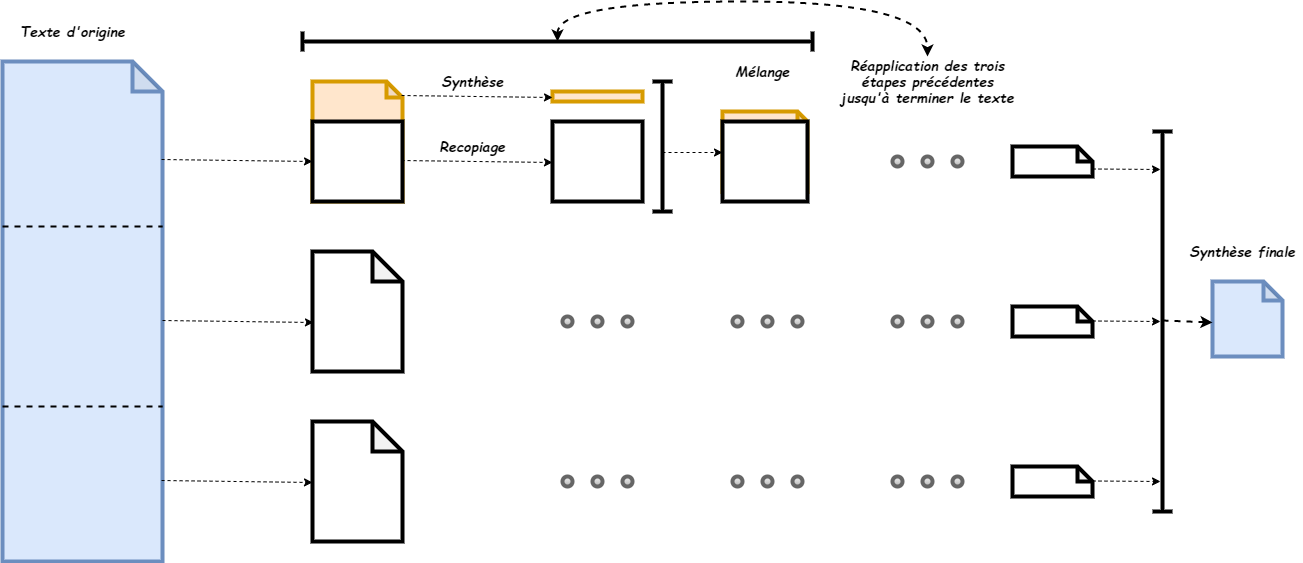
\includegraphics[width=16.5cm]{PipelineSummary.png}
\captionof{figure}{Pipeline de synthèse abstractive}\label{PipelineSumm}
\end{center}
$ _{} $ $ _{} $ $ _{} $ $ _{} $ $ _{} $Sur la figure \ref{PipelineSumm}, la particularité réside au fait que dans l'implémentation, les divisions se feront en découpant au préalable tout texte en ses phrases constitutives, puis, en reliant un certain nombre de phrases se présentant en tête de chaque partie jusqu'à atteindre une longueur inférieure à la limite admissible par le modèle utilisé. Finalement, la synthèse obtenue pour cette sous-partie sera ajoutée à la partie globale et le processus se répétera comme l'illustre la figure. Nous avons testé cette méthode et elle nous a permis de mieux conforter le compromis vitesse-qualité par rapport aux pipelines classiques \cite{GRAAL_HF_tunstall2022natural}.
\item[•] \textit{Module de synthèse extrait simplifié} : Il s'agira d'un module qui permettra la réalisation de la synthèse mais en utilisant l'un des algorithmes de synthèse extraite (le plus rapide).
\item[•] \textit{Module expérimental} : Il s'agira d'un module de synthèse abstraite qui sera es\-sen\-tiel\-le\-ment utilisé pour la synthèse des petits documents (quelques pages). Ce module sera entraîné à partir des synthèses collectées par le système, pour améliorer au fur et à mesure ses performances. Nous comptons réaliser l'entraînement par \textit{transfer learning} avec le \textit{transformer} \textit{mBART} \cite{mBART_liu2020multilingual} comme base. 
\end{itemize}
On peut aussi remarquer qu'il y a un module \textit{pre-processing} dans la partie interfaces. C'est à la suite du fait que, pour des raisons de performance, on devra envoyer à l'\textit{API} le fichier sous un format particulier. Il faudra réaliser l'acquisition des données dans divers formats (\textit{pdf},\textit{docx},...) mais les données acquises seront envoyées dans un format plus léger à l'\textit{API} (du \textit{JSON} pour notre cas). \textbf{Ce \textit{pre-processing} consistera donc à extraire les données des documents fournis en entrée. Cela devra être fait sans les corrompre pour s'assurer de la qualité des résumés.}\\
$ _{} $ $ _{} $ $ _{} $ $ _{} $ $ _{} $La base des données, que nous avons mentionné dans la figure \ref{ArchiSysteme} a un double rôle :
\begin{itemize}
\item[1°)] Le stockage des données de l'utilisateur (il s'agira en fait des identifiants des in\-ter\-fa\-ces qui utiliseront l'\textit{API});
\item[2°)] Le stockage des paires document-synthèse, ainsi que l'appréciation de l'utilisateur (évaluation par les utilisateurs).
\end{itemize}
\subsection{Architecture du module de synthèse extractive}\label{SectionMerging}
$ _{} $ $ _{} $ $ _{} $ $ _{} $ $ _{} $Le module de synthèse extractive, que nous nommerons \textit{\textbf{merging}}, se présente comme suit :\newpage
$ _{ } $\\
\begin{center}
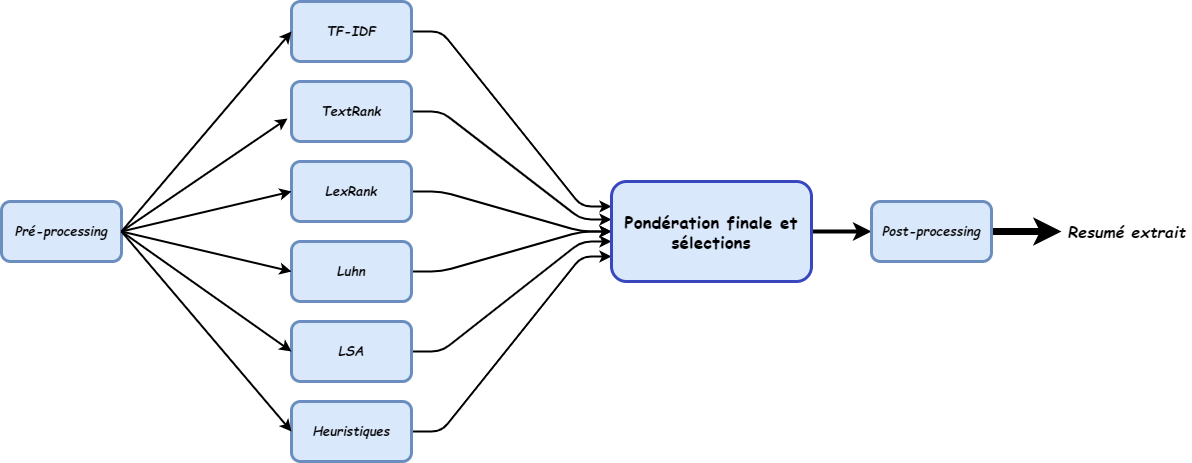
\includegraphics[width=16cm]{ResumeExtrait.png}
\captionof{figure}{Architecture globale du module de synthèse extractive}\label{ArchiGlobExtract}
\end{center}
$ _{ } $\\
Comme nous pouvons le voir sur la figure \ref{ArchiGlobExtract}, un traitement sera fait pour adapter les données reçues à ce qui peut être traité par le système. Ce traitement consistera es\-sen\-tiel\-le\-ment à réaliser la \textit{tokenisation} des textes (chaque \textit{token} sera une phrase pour cette partie) et à affecter un identifiant unique à chaque phrase.\\
Après cela, les données seront invariablement passées aux divers algorithmes de synthèse ex\-tra\-ctive (\textit{TFIDF, LexRank, ...}), qui générerons chacun un groupe de poids des phrases. Après cela, le module de pon\-dé\-ra\-tion et sélection réalisera successivement ce qui suit :
\begin{itemize}
\item[1°)] Acquisition des sorties de chaque algorithme de synthèse extractive (il s'agira des dictionnaires dont les clés seront les identifiant uniques des phrases et les valeurs seront les poids affectés par l'algorithme). A chaque algorithme, on donnera un poids qu'on nommera $ W_{Nom de l'algo} $ compris entre $ 0 $ et $ 1 $, selon la confiance qu'on lui porte (la somme des poids sera égale à $ 1 $ et par défaut, tous les algorithmes pourront avoir le même poids) ;
\item[2°)] Élimination des phrases de poids faible (avec comme seuil, la taille maximale de résumé précisée par l'utilisateur) ;
\item[3°)] Réarrangement de chaque dictionnaire obtenu après expulsion des phrases non si\-gni\-fi\-ca\-ti\-ves (les éléments seront arrangés par ordre décroissant des poids pour chaque sortie);
\item[4°)] Donner des probabilités aux espaces des poids de chaque dictionnaire par application d'un \textit{softmax} sur chacun d'eux. Ce qui donnera, pour chaque phrase de chaque dictionnaire, un nouveau poids $ \omega_{phr_{i}} $, avec $ i $ le numéro du dictionnaire et $ phr $ le numéro de la phrase considérée dans ce dictionnaire ;
\item[5°)] Listage complet des éléments (leurs identifiants) de tous les dictionnaires.
\item[6°)] Pour chaque élément de la liste globale ainsi établie, appliquer la formule suivante pour obtenir un nouveau poids :
\begin{eqnarray}
\mathcal{W}_{j} = \sum_{i\in \mathcal{D}}\left( W_{i}\cdot \omega_{phr_{i}}\right)
\end{eqnarray}
Avec $ \mathcal{W}_{j} $ le nouveau poids affecté à la phrase ayant un identifiant global $ j $ (l'identifiant là d'origine) et $ \mathcal{D} $ la liste des dictionnaires (les sorties de chaque algorithme) ;
\item[7°)] Arranger toutes les phrases par ordre décroissant dans une unique liste et sélectionner les plus haut dans la liste jusqu'à atteindre le seuil fixé (nombre de mots fixé pour la synthèse).
\item[8°)] Constituer une liste avec les éléments sélectionnés.
\item[9°)] Réarranger les phrases de la liste selon leur ordre de succession dans le texte d'origine.
\item[10°)] Constituer la synthèse extraite.
\end{itemize}
Ce qui précède constitue en fait l'algorithme que nous allons implémenter pour le \textit{module de pondération et sélection}. Précisons seu\-le\-ment que, les poids des algorithmes (voir le paramètre $ W_{Nom de l'algo} $ du point $ 1° $ de la description ci-dessus) seront accordés de manière statique et non dynamique. Pour les choisir, nous allons nous servir des scores de chacun de ces algorithmes aux diverses métriques que nous présenterons au chapitre suivant. Et c'est à cette même occasion que nous préciserons les valeurs choisies pour ces paramètres ( Valeurs à retrouver dans le tableau \ref{MergingWeights}).
\subsection{Architecture du module de synthèse abstractive}
$ _{} $ $ _{} $ $ _{} $ $ _{} $ $ _{} $Le module de synthèse abstraite n'est pas unique. Nous implémenterons plusieurs modèles (\textit{BART}, \textit{BARThez}, \textit{PEGASUS} et \textit{mBART} entraîné avec nos données); Chaque module de synthèse se présentera néanmoins comme suit :
$ _{ } $\\
\begin{center}
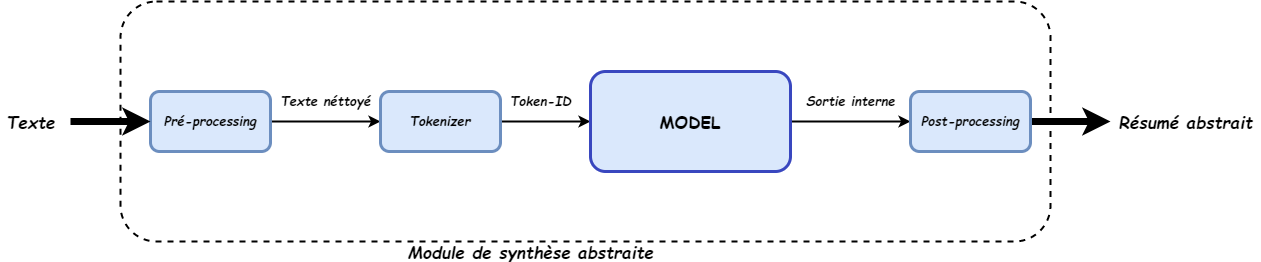
\includegraphics[width=16cm]{ResumeAbstraitGLOBAL.png}
\captionof{figure}{Architecture globale du système de synthèse abstractive}\label{ArchiGloAbstract}
\end{center}
$ _{ } $\\
Comme nous pouvons le remarquer, il y a toujours un module de mise en forme initial (\textit{pre-processing}) qui nous permettra en gros de supprimer tous les caractères que nous ne pourrons pas gérer. Vient ensuite le module de tokenisation (le \textit{tokenizer} ou tokeniseur) \cite{GRAAL_HF_tunstall2022natural}  qui consistera ici à diviser tout le texte en ses mots constitutifs et à leur affecter des identifiants numériques. Ce sont ces identifiants qui seront fournis au modèle et transformés en vecteurs par la couche d'\textit{embedding} du modèle.\\
$ _{} $ $ _{} $ $ _{} $ $ _{} $ $ _{} $Le modèle quant à lui, aura toujours une architecture pareille :
$ _{ } $\\
\begin{center}
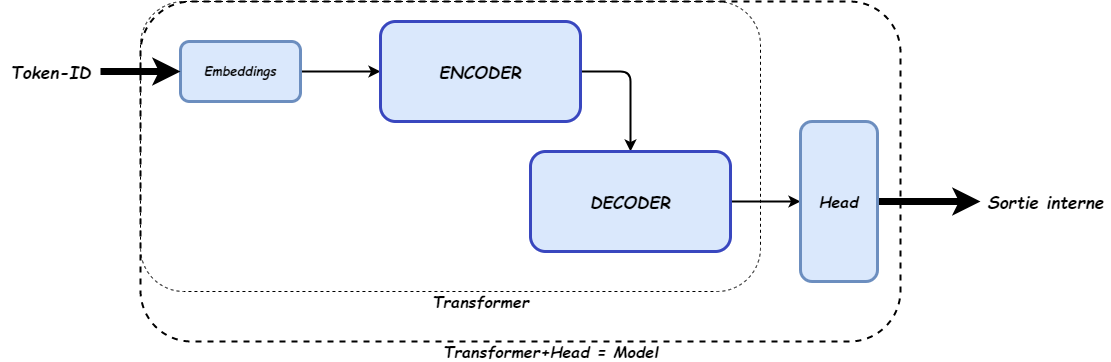
\includegraphics[width=16cm]{Model.png}
\captionof{figure}{Architecture interne du modèle mentionné sur la figure \ref{ArchiGloAbstract}}
\end{center}
$ _{ } $\\
Il s'agit en effet de l'architecture classique d'un \textit{transformer}, comme présenté sur la figure \ref{ImgTransformerVASWANI} à l'exception du fait qu'ici on fait ex\-pli\-ci\-te\-ment ap\-pa\-raî\-tre l'existence de la sortie du modèle. Ça correspond au \textit{réseau linéaire} suivi d'une couche de \textit{softmax} tel que présenté sur la figure \ref{ImgTransformerVASWANI}. Cette partie, que nous avons nommé \textit{head} est différente selon les tâches \cite{HF_wolf2020transformers}, c'est pourquoi nous avons voulu la mentionner explicitement car, selon le besoin, on peut la modifier.\\
Nous devons finalement mentionner que les modules de \textit{tokenisation} (nommés \textit{tokenizer} en anglais) dépendront explicitement des modèles utilisés.
\subsection{Présentation des interfaces}
$ _{} $ $ _{} $ $ _{} $ $ _{} $ $ _{} $La partie interface nous permettra juste d'utiliser le service que nous aurons élaboré et d'évaluer par la même occasion ses performances. Voici donc une ébauche d'interface que nous comptons utiliser pour exploiter le service :
$ _{ } $\\
\begin{center}
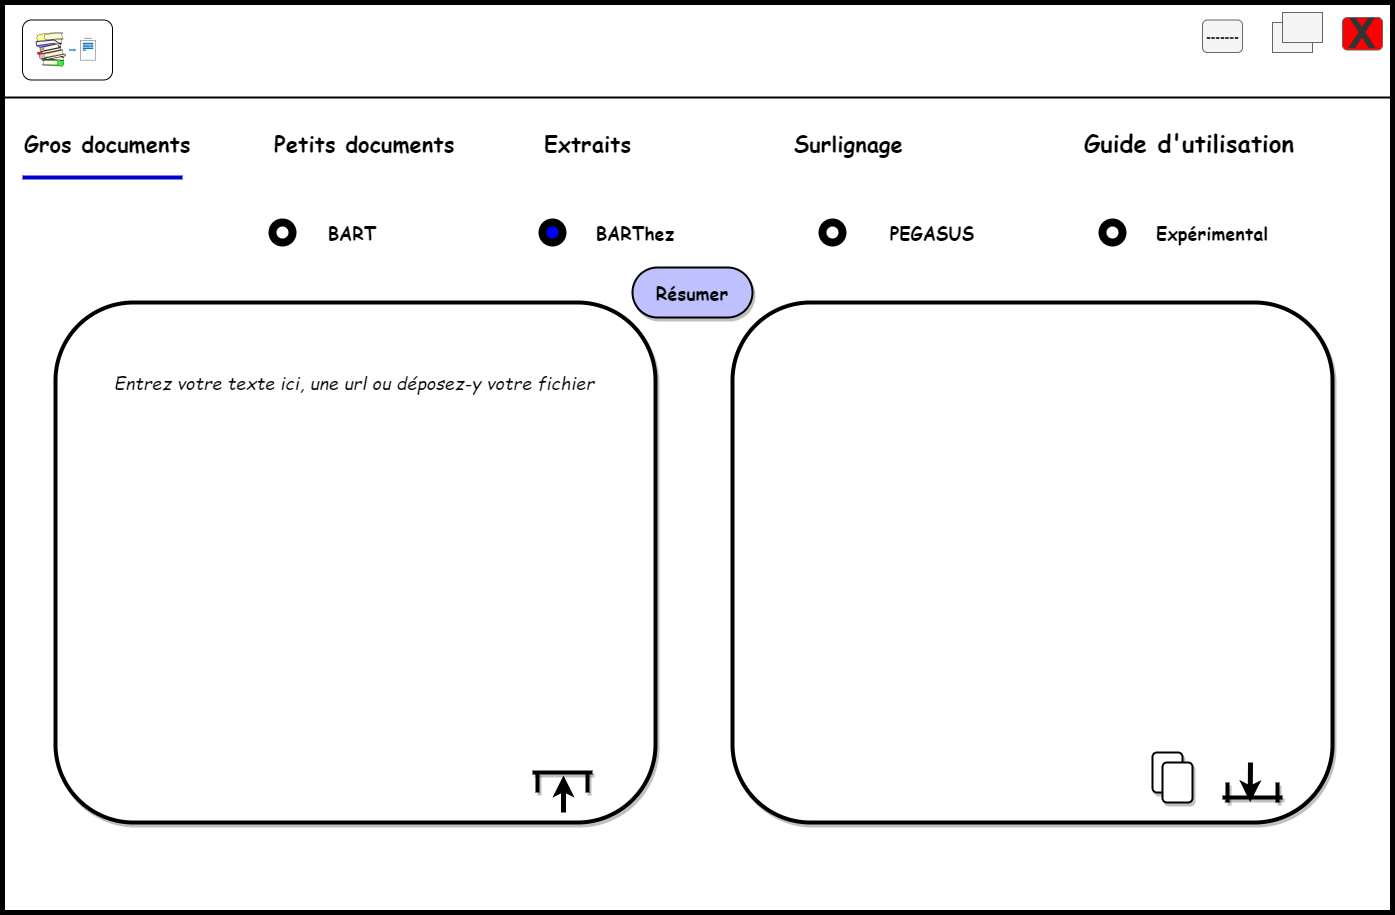
\includegraphics[width=16cm]{PageOne.png}
\captionof{figure}{Ébauche d'interface}\label{EbaucheInterface}
\end{center}
$ _{ } $\\
Avec cette interface, on a une idée générale de la manière dont nous comptons servir le système aux utilisateurs.
\section{Conclusion partielle}
$ _{} $ $ _{} $ $ _{} $ $ _{} $ $ _{} $Dans cette partie, nous venons de présenter le résumé automatique des textes, tout en réalisant une vue d'ensemble des méthodes utilisées dans la littérature à cet effet. Nous avons mentionné que la classification des résumés que nous utiliserons sera celle les départageant en \textit{abstractive summarization} et \textit{extractive summarization} et que, pour notre cas, il s'agira de réaliser un système de résumé mono-document, avec une partie abstractive et une autre extractive, générant un résumé générique pour des documents de type narratif et argumentatif.\\
$ _{} $ $ _{} $ $ _{} $ $ _{} $ $ _{} $Nous avons également listé les divers modèles de \textit{transformer} adaptés à la tâche de synthèse automatique abstraite, et nous avons mentionné devoir utiliser les modèles du type \textit{BART} pour des raisons qui serons précisées dans le chapitre suivant.\\
Enfin, nous avons réalisé la conception préliminaire du système tout en précisant que, concernant l'\textit{API}, la \textit{BD} (Base des Données) et les interfaces, les détails d'implémentation utiles seront précisés dans la partie dédiée à la conception proprement dite et aux tests, c'est-à-dire au chapitre suivant. Le chapitre suivant nous permettra donc finalement de préciser, réaliser et tester les méthodes que nous avons jusque-là adoptées pour la mise au point de notre système de synthèse automatique des documents.
\chapter{CONCEPTION DU FILTRE MIXTE ADAPTÉ}
\section{Introduction partielle}
$ _{} $ $ _{} $ $ _{} $ $ _{} $ $ _{} $Dans les chapitres précédents, nous avons esquissé tout l'environnement du système que nous avons prévu élaborer à travers ce mémoire. A présent, nous allons présenter avec précision les diverses parties de notre système.\\
$ _{} $ $ _{} $ $ _{} $ $ _{} $ $ _{} $Dans ce chapitre, nous comptons en premier lieu finaliser la conception entamée au chapitre précédent. En second lieu, nous allons décrire les diverses méthodes utilisées pour évaluer les résumés générés au\-to\-ma\-ti\-que\-ment, nous allons décrire l'implémentation de notre système, nous allons tester les algorithmes et modèles dont nous avons fait usage et nous allons justifier les choix d'implémentation que nous avons faits.\\
$ _{} $ $ _{} $ $ _{} $ $ _{} $ $ _{} $Les tests en particulier seront faits de manière à pouvoir donner une justification cohérente des choix d'implémentation que nous avons faits et à classer, par la même occasion, nos algorithmes les uns par rapport aux autres. Cela est donc l'objet de ce chapitre et nous estimons qu'il nous permettra de présenter les points techniques saillants de notre système.
\section{Conception détaillée}
$ _{} $ $ _{} $ $ _{} $ $ _{} $ $ _{} $Comme nous l'avons annoncé au précédent chapitre, dans cette partie nous allons finaliser la conception entamée. Cela consiste principalement en la conception de la base des données, de l'\textit{API} et des interfaces. Plus précisément, il s'agira de conception et présentation.\newpage
\subsection{Conception de la base des données}
$ _{} $ $ _{} $ $ _{} $ $ _{} $ $ _{} $La conception d'une base des données passe en général par les étapes qui suivent \cite{rigaux2001cours} :
\begin{itemize}
\item[•] L'analyse des besoins en stockage;
\item[•] Le regroupement des données repérées comme utiles en tables selon leur affinité;
\item[•] La spécification des clés primaires et l'analyse des relations entre tables;
\item[•] La normalisation de la base des données.
\end{itemize}
Étant donné ce que nous avons précisé au chapitre précédent comme spécifications du système, et ensuite ce que nous avons mentionné comme rôles principaux de la base des données dans notre système, il se dégage les besoins suivants en terme de stockage :\\
Il nous sera utile de stocker principalement \underline{les textes} et \underline{leurs résumés}, les \\
\underline{évaluations des résumés} par les utilisateurs, \underline{les dates} et \underline{le modèle source}. Il nous sera également utile de stocker \underline{les clés d'authentification} des systèmes utilisant l'API, \underline{les noms} et \underline{ logins} des développeurs se servant des services de l'API mais également leurs\\ \underline{mots de passe}.\\
$ _{} $ $ _{} $ $ _{} $ $ _{} $ $ _{} $Cela nous montre que nous n'aurons besoin que de $ 3 $ tables au maximum :\\
Une pour tout ce qui concerne les textes, une pour la gestion des clés des développeurs  enregistrés sur la plateforme, et une autre pour la gestion de leur identité. Nous préférons séparer les tables sur l'identité des développeurs avec celle contenant leurs clés car on peut avoir égaré la clé d'authentification et vouloir en générer une autre, d'où c'est plus judicieux de considérer les informations sur les clés comme une entité à part.\\
Des considérations qui précèdent on tire le diagramme des classes suivant :\newpage
$ _{ } $
\begin{center}
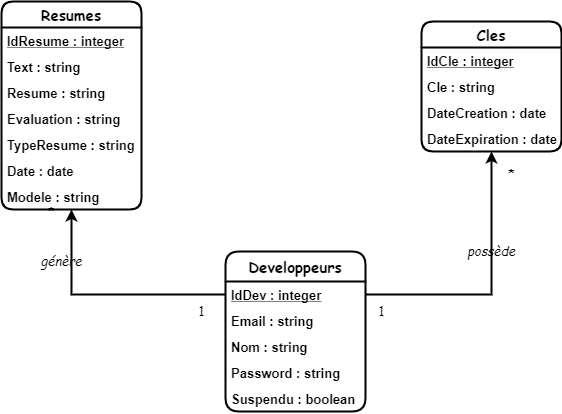
\includegraphics[width=14cm]{BDdiagrams.png}
\captionof{figure}[Structure de la base des données]{Diagramme des classes représentant la base des données} \label{BDdiagrams}
\end{center}
$ _{ } $\\
On peut remarquer sur la figure \ref{BDdiagrams} l'ajout des attributs \underline{type de résumé} et \underline{date} dans la classe des résumés, ainsi que des attributs \underline{date de création} et \underline{date d'expiration} dans la classe des clés d'authentification, puis finalement l'attribut \underline{suspendu?} dans la classe des développeurs.

\begin{itemize}
\item[•] L'attribut \textit{type de résumé} permettra de sélectionner les résumés par type sans avoir à se fier des modèles mis en place dans le système;
\item[•] L'attribut \textit{date} ajouté dans la classe des résumés pourra permettre de suivre l'évolution des performances car on aura également le modèle qui aura produit les résumés considérés.
\item[•] Les attributs \textit{date de création} et \textit{date d'expiration} ajoutés à la classe des clés permettront de faciliter plus tard le management des développeurs utilisateurs des services de l'API dans leurs systèmes et cela va en connivence avec l'attribut \textit{suspendu?} ajouté à la classe des développeurs.
\end{itemize}
Les \textit{id} seront considérés comme clé primaire et l'\underline{id de développeur} sera une clé étrangère dans les tables réservées aux résumés et aux clés. Ainsi, nous considérons terminée la phase de conception de la base des données.
\subsection{Conception de l'API de synthèse}
$ _{} $ $ _{} $ $ _{} $ $ _{} $ $ _{} $La création d'une interface de programmation des applications (\textit{Application Programming Interface}) se fait en s'interrogeant sur les services qu'on veut pourvoir à travers cette \textit{API}.\\
Pour ce qui nous concerne, nous voulons mettre au point une plateforme capable de retourner les résumés aux textes qui lui seront présentés. Nous devons également pouvoir identifier les gens qui se serviront de l'API dans leurs systèmes (les développeurs dont on parlait dans la section précédente), d'où la nécessité de les enregistrer, de leur donner la possibilité de s'authentifier et de générer une clé d'authentification à utiliser dans leurs systèmes.\\
$ _{} $ $ _{} $ $ _{} $ $ _{} $ $ _{} $Nous allons également donner la possibilité de tester plusieurs modèles de résumé des textes et permettre ainsi aux utilisateurs de comparer diverses synthèses. Pour cela, nous avons prévu $ 4 $ familles d'\textit{end-points} :
\begin{itemize}
\item[1°)] \textit{End-points} réservés à la synthèse extractive;
\item[2°)] \textit{End-points} réservés à la synthèse abstractive;
\item[3°)] \textit{End-points} réservés à tout ce qui concerne les vues de l'API (ses interfaces devant permettre l'authentification, la génération des clés et la documentation);
\item[4°)] \textit{End-points} réservés à l'administration du système (que nous avons implémenté mais que nous passerons sous silence dans ce travail).
\end{itemize}
On peut aussi y joindre un \textit{end-poind pour l'évaluation} des résumés produits.
\subsubsection{End-points pour la synthèse extractive}
$ _{} $ $ _{} $ $ _{} $ $ _{} $ $ _{} $Pour la synthèse extractive, nous avons prévu essentiellement deux \textit{end-points} pour comparer notre algorithme de synthèse extractive à l'un des systèmes de synthèse extractive le plus performant. Il s'est agit des \textit{end-points} réservé au système basé sur le module python \textit{gensim} et celui réservé à notre approche qui est un mélange de plusieurs algorithmes de synthèse extractive (on l'a nommé \textit{merging}) comme on peut le voir sur la figure \ref{ArchiGlobExtract} du chapitre précédent.\\
On a l'\textit{end-point} de synthèse extractive basé sur le module \textit{gensim} donné par :
\begin{center}

\includegraphics[scale=0.5]{POSTextractiveGensim.png}
\end{center}
Puis celui de synthèse extractive par combinaison de divers algorithmes donné par :
\begin{center}

\includegraphics[scale=0.5]{POSTextractiveMerge.png}
\end{center}
\subsubsection{End-points pour la synthèse abstractive}
Pour la synthèse abstractive, nous avons prévu $ 5 $ \textit{end-points} dont :
\begin{itemize}
\item[1.] Un \textit{end-point} utilisant le modèle \textit{BART} dont nous avons optimisé l'utilisation en le servant à travers le processus présenté à la figure \ref{PipelineSumm} du chapitre précédent. L'\textit{end-point} en question est :
\begin{center}

\includegraphics[scale=0.5]{POSTabstractiveLarge.png}
\end{center}
\item[2.] Un autre \textit{end-point} basé sur \textit{BART} mais pouvant prendre en charge des documents plus gros :
\begin{center}

\includegraphics[scale=0.5]{POSTabstractiveVeryLarge.png}
\end{center}
\item[3.] Un \textit{end-point} basé sur \textit{BARThez}, le modèle de synthèse le plus utilisé pour la synthèse entièrement en français :
\begin{center}

\includegraphics[scale=0.5]{POSTabstractiveBarthez.png}
\end{center}
\item[4.] Un \textit{end-point} basé sur \textit{Pegasus}, l'un des modèles à grand pouvoir d'abstraction :
\begin{center}

\includegraphics[scale=0.5]{POSTabstractivePegasus.png}
\end{center}
\item[5.] Un \textit{end-point} basé sur \textit{BARTkrame}, notre modèle de synthèse élaboré pour fonctionner entièrement en français :
\begin{center}

\includegraphics[scale=0.5]{POSTabstractiveExperimentalBartkrame.png}
\end{center}
\end{itemize}
\subsubsection{End-points pour les vues de l'API et l'authentification}
Tout d'abord, le point d'entrée est donné naturellement par l'\textit{end-point} :
\begin{center}

\includegraphics[scale=0.5]{GEThome.png}
\end{center}
Ensuite, l'\textit{end-point} réservé à l'authentification :
\begin{center}

\includegraphics[scale=0.5]{POSTlogin.png}
\end{center}
Vient alors l'\textit{end-point} dédié à l'enregistrement :
\begin{center}

\includegraphics[scale=0.5]{POSTsignUp.png}
\end{center}
Par après on a l'\textit{end-point} réservé à la déconnexion :
\begin{center}

\includegraphics[scale=0.5]{GETlogout.png}
\end{center}
Puis celui réservé à la génération des clés :
\begin{center}

\includegraphics[scale=0.5]{GETupdateToken.png}
\end{center}

Finalement, on a un \textit{end-point} commun aux familles de synthèse extractive et abstractive pour l'évaluation des synthèses. C'est donné par :
\begin{center}

\includegraphics[scale=0.5]{POSTevaluation.png}
\end{center}
$ _{ } $\\
Nous estimons que la description ici faite suffit comme conception des grandes lignes de notre \textit{API}. Le reste de la documentation est dans l'annexe \ref{AnnexeDocu}.
\subsection{Conception des interfaces}\label{SectionConceptionInterfaces}
$ _{} $ $ _{} $ $ _{} $ $ _{} $ $ _{} $Étant donné l'API mise sur pieds, nous avons également implémenté un client web devant s'en servir pour en illustrer le fonctionnement. Pour cela, nous avons voulu exploiter toutes les possibilités de l'API en se basant sur les spécifications du système (nous les avons cité au chapitre précédent) et les objectifs de ce travail. C'est ainsi que les interfaces ont été conçues de manière à pouvoir :
\begin{itemize}
\item[•] Permettre la synthèse abstractive en utilisant tous les modèles mis à notre disposition par l'API;
\item[•] Permettre la synthèse extractive en utilisant les deux approches pourvues par l'API;
\item[•] Permettre le téléchargement des synthèses obtenues;
\item[•] Permettre aux utilisateurs de coter les synthèses qui leur ont été fournies;
\item[•] Permettre le chargement des fichiers sous différents formats (\textbf{word}, \textbf{pdf} et \textbf{txt}).
\end{itemize}
Pour cela, et sur base de l'ébauche des interfaces qui a été présentée à la figure \ref{EbaucheInterface} nous avons adopté ce qui suit comme interfaces du client de notre système.
\begin{center}
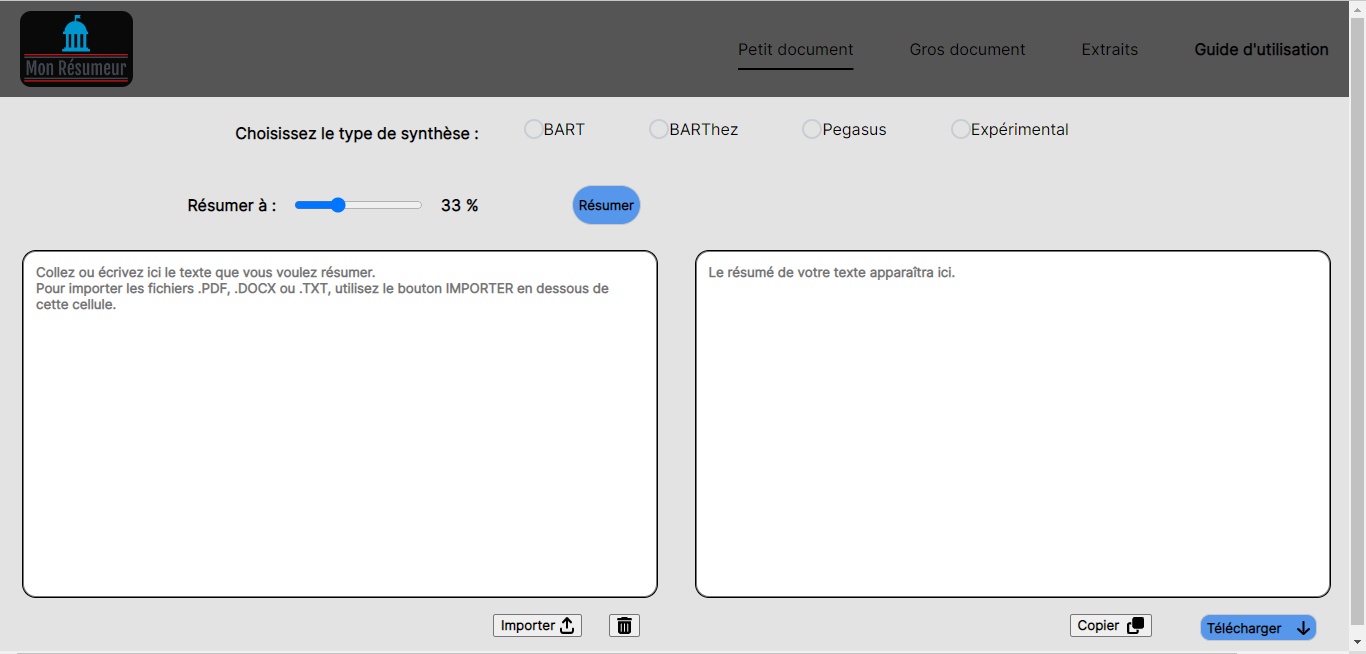
\includegraphics[width=16cm]{Interface1PetitsDocs.png}
\captionof{figure}{Interface générique du système}\label{Interface1PetitsDocs}
\end{center}
Sur la figure \ref{Interface1PetitsDocs} nous montrons la manière dont les interfaces se présentent en général.\\
Durant le processus de synthèse, l'interface se présente comme suit :
\begin{center}
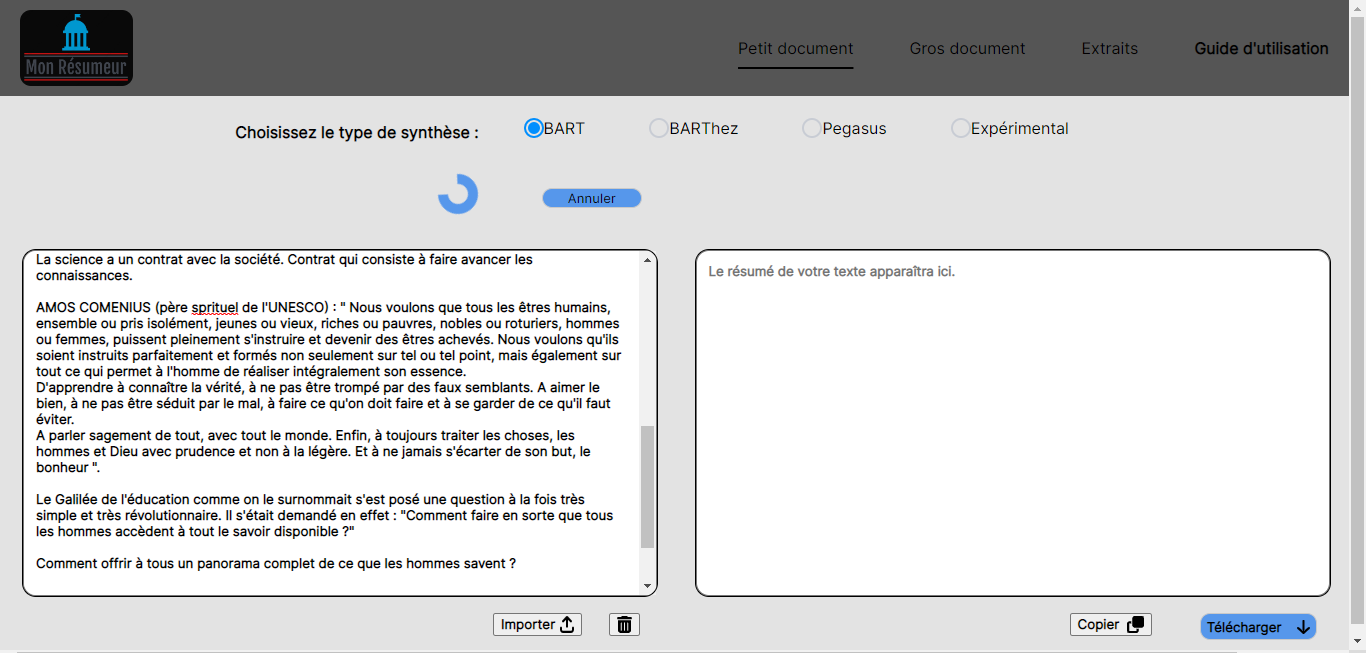
\includegraphics[width=16cm]{Interface1Pendant.png}
\captionof{figure}{Interface durant le processus de synthèse}\label{Interface1EnCours}
\end{center}
On peut remarquer sur la figure \ref{Interface1EnCours} que durant la synthèse, une possibilité d'annulation se présentera.\\
Après génération de la synthèse, l'interface se présentera comme suit :
\begin{center}
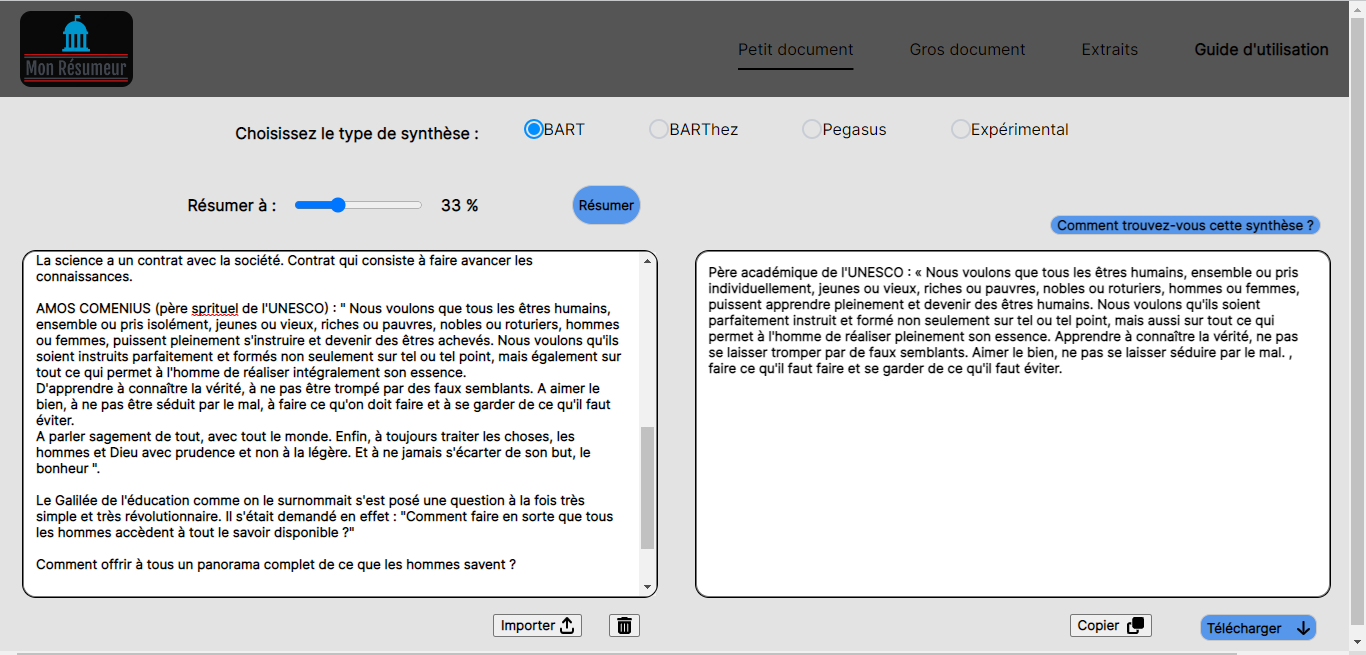
\includegraphics[width=16cm]{Interface1Apres.png}
\captionof{figure}{Interface après génération de la synthèse}\label{Interface1Apres}
\end{center}
Il est clair également sur la figure \ref{Interface1Apres} qu'après synthèse, un bouton devant permettre d'évaluer la synthèse se présentera. En y cliquant, on pourra avoir la possibilité d'évaluer le résumé obtenu, comme cela se voit sur la figure suivante :
\begin{center}
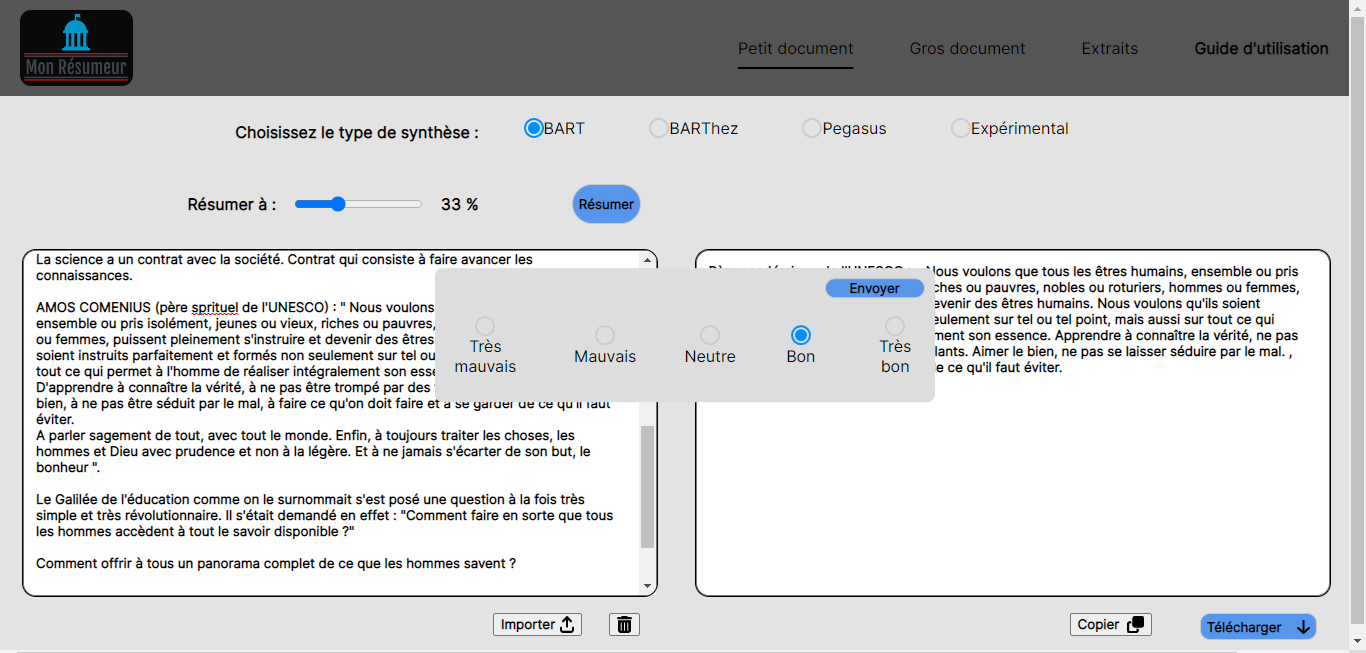
\includegraphics[width=16cm]{Interface1Evaluation.png}
\captionof{figure}{Interface durant l'évaluation de la synthèse obtenue}\label{Interface1Evaluation}
\end{center}
Pour guider l'utilisateur, au survol du curseur de réglage de la taille du résumé, l'interface se présente comme suit :
\begin{center}
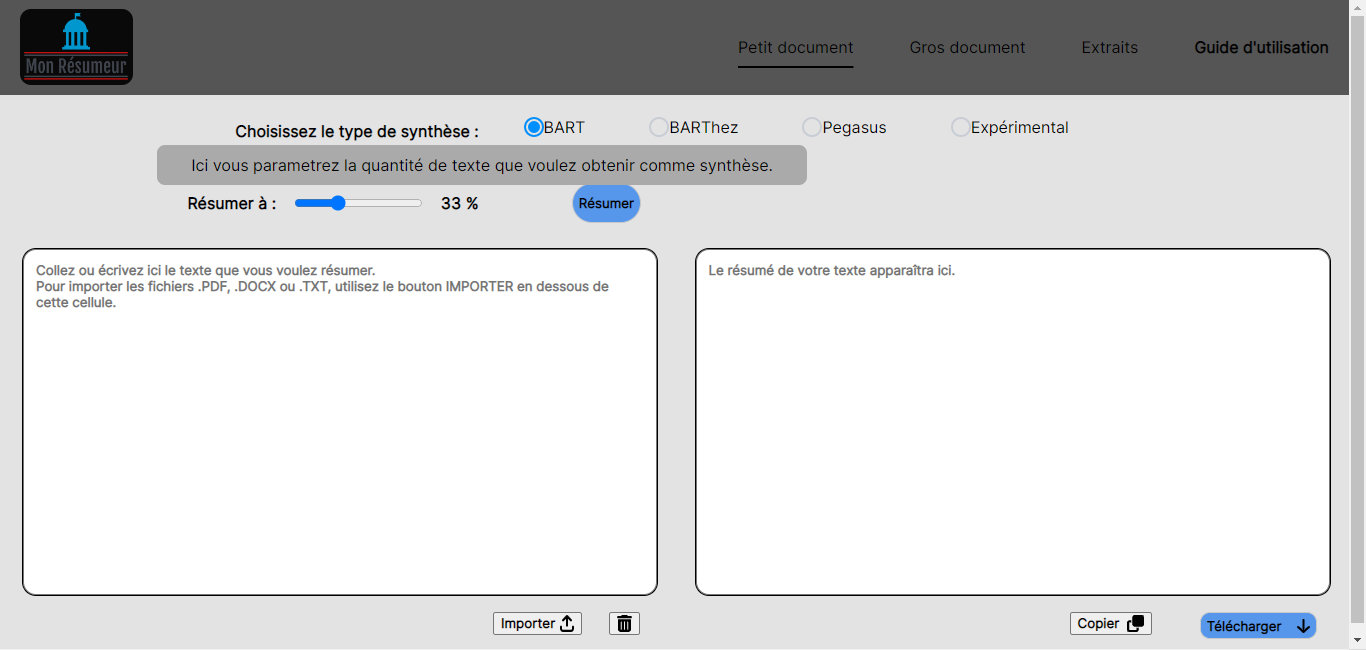
\includegraphics[width=16cm]{Interface1CurseurHover.png}
\captionof{figure}{Interface au survol du curseur de réglage de résumé}\label{Interface1CurseurHover}
\end{center}

En cas de limitation des ressources serveur lors de l'hébergement de l'API, nous avons prévu disponibiliser uniquement le système réduit :
\begin{center}
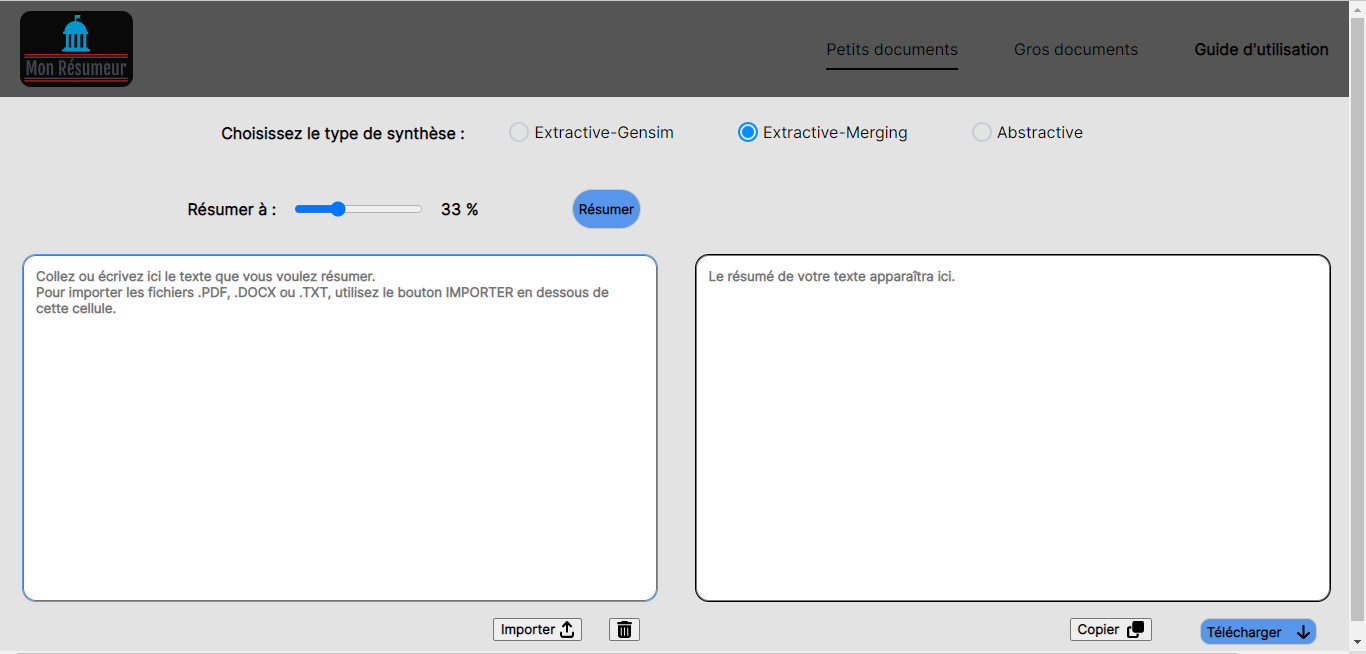
\includegraphics[width=16cm]{InterfacesReducedPetitsDocs.png}
\captionof{figure}{Interface réduite côté petits documents}\label{InterfacesReducedPetitsDocs}
\end{center}

\begin{center}
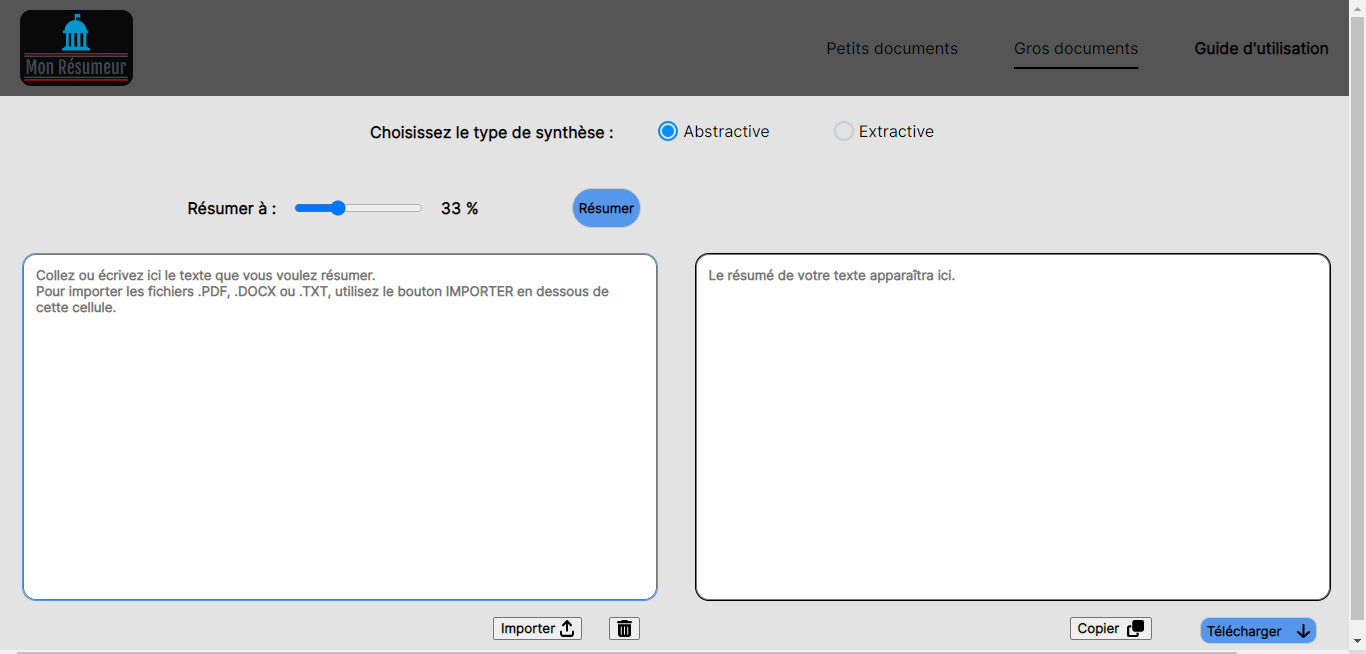
\includegraphics[width=16cm]{InterfacesReducedGrosDocs.png}
\captionof{figure}{Interface réduite côté gros documents}\label{InterfacesReducedGrosDocs}
\end{center}

Les autres fonctionnalités peuvent être explorées en utilisant le système.

\section{Évaluation des résumés}\label{sectionSurROUGE}
$ _{} $ $ _{} $ $ _{} $ $ _{} $ $ _{} $L'évaluation des résumés est une tâche assez complexe. Les méthodes cla\-ssi\-que\-ment utilisées pour évaluer les performances d'un système informatique, et en particulier celles utilisées pour évaluer les systèmes basés sur les réseaux de neurones, ne peuvent pas s'appliquer de manière brute pour les systèmes de génération de texte comme ceux de résumé automatique. En effet, il n'existe pas de référence parfaite de résumé pour un document donné. Les professionnels humains d'ailleurs produisent des résumés différents pour un même texte, chacun selon ses penchants et ses goûts. Plus étonnant encore, un même humain ne produit en général pas le même résumé si la tâche lui est donnée à quelques temps d'intervalle \cite{rath1961formation}. C'est donc une tâche teintée d'une grande part de subjectivité. Cependant, la majorité s'accorde quand on est face à un bon résumé.\\
$ _{} $ $ _{} $ $ _{} $ $ _{} $ $ _{} $Comment alors faire pour parvenir à repérer, avec plus d'objectivité, qu'un résumé donné est de bonne qualité ? Comment même parvenir à comparer, sans équivoque, les qualités de deux résumés qui nous seraient présentés ? La solution à cette question est importante car elle permettra de pouvoir évaluer objectivement et rapidement les systèmes de résumé automatique mais, au-delà de cela, elle permettra d'en suivre l'évolution durant l'entraînement au cas où il s'agit des systèmes de résumé basés sur l'apprentissage automatique.\\
$ _{} $ $ _{} $ $ _{} $ $ _{} $ $ _{} $Généralement, on subdivise l'évaluation des résumés en deux principales catégories qui sont l'évaluation extrinsèque et l'évaluation intrinsèque\cite{jones1995evaluating}. L'évaluation intrinsèque est celle qui s'obtient par la lecture directe du résumé. Il peut s'agir d'un résumé manuel (évaluation directe par un humain selon un certain nombre de critères), un résumé semi-automatique ou bien un résumé automatique. L'évaluation extrinsèque quant à elle consiste à évaluer les résumés indirectement. Pour ce faire, on peut par exemple passer par l'évaluation de la possibilité de donner une réponse à un certain nombre de questions après lecture du résumé \cite{maybury1999advances},... Beaucoup de recherches ont été menées sur l'évaluation des résumés mais les solutions ne sont que partielles le plus souvent \cite{lin2004rouge,hirschberg2005summaries,louis2008automatic, saggion2010multilingual}. Dans ce travail, nous ne parlons que des méthodes d'évaluation intrinsèques qui nous intéressent.
\subsection{Évaluation manuelle}
$ _{} $ $ _{} $ $ _{} $ $ _{} $ $ _{} $L'évaluation manuelle consiste à se fier au jugement d'un certain nombre d'experts humains, selon un certain nombre de critères préétablis \cite{torres2014automatic}. Pour plus d'information à ce sujet, se rapporter aux campagnes annuelles d'évaluation \textbf{DUC} ou \textit{Document Understanding Conference} (renommé \textbf{TAC} \cite{TAC} ou \textit{Text Analysis Conference} depuis $ 2008 $). Ces méthodes demeurant subjectives, les méthodes semi-automatiques ont été mises au point.
\subsection{Évaluation semi-automatique}
$ _{} $ $ _{} $ $ _{} $ $ _{} $ $ _{} $Nous allons présenter ici les méthodes les plus connues et les plus utilisées \cite{hong2014repository} pour évaluer les résumés. Il s'agit de \textbf{ROUGE}(\textit{Recall Oriented Understudy for Gisting Evaluation}), \textit{que nous allons utiliser pour nos évaluations} et de \textbf{PYRAMID} dont nous allons montrer la faiblesse par rapport à \textit{ROUGE}, bien que celui-là soit plus corrélé aux jugements humains \cite{nenkova2004evaluating}.
\subsubsection{ROUGE \cite{lin2004rouge}}\label{ROUGEmetricsSection}
$ _{} $ $ _{} $ $ _{} $ $ _{} $ $ _{} $Cette métrique est orientée rappel comme son nom l'indique. On cherche à évaluer jusqu'à quel point le résumé obtenu rappelle celui qui est pris comme référence. Pour réaliser ladite mesure, on se base essentiellement sur la correspondance mot à mot (on parle des \textit{unigrammes}), de deux mots à deux mots (on parle alors de comparaison par \textit{bigrammes}),... Pour être général, on parle des \textit{n-grammes}. Considérons la phrase :
\begin{center}
\textit{Il arrive demain avec deux objets rares.}
\end{center}
Les unigrammes de cette phrase sont \textit{il}, \textit{arrive}, \textit{demain}, \textit{avec}, \textit{deux}, \textit{objets} et \textit{rares}, soit les mots du texte. Les bigrammes sont \textit{il arrive}, \textit{arrive demain}, \textit{demain avec}, \textit{avec deux}, \textit{deux objets}, \textit{objets rares}.
Dans le paquet des mesures proposées par \textit{ROUGE}, il y a :
\begin{itemize}
\item[1°)] \underline{ROUGE-N}\\
Formellement, \textit{ROUGE-N} est une mesure de rappel (\textit{recall}) des N-grammes entre le résumé candidat et le ou les résumé(s) de référence. C'est régi par la relation qui suit :
\begin{eqnarray}
ROUGE-N = \frac{\sum_{r\in R}\mbox{ }Co_{c-r}}{\sum_{r\in R}\mbox{ }(N-grammes)_{r}}
\end{eqnarray}
Avec $ r $ un résumé de référence parmi ceux pris pour référence (paquet $ R $), $ (N-grammes)_{r} $ le nombre total de \textit{N-grammes} dans un résumé de référence \textit{r} et $ Co_{c-r} $ le nombre de \textit{N-grammes} du résumé candidat qui se retrouvent dans le résumé de référence \textit{r}.\\
C'est ainsi qu'on trouve \textit{ROUGE-1} basé sur une comparaison des \textit{unigrammes}, \textit{ROUGE-2} basé sur celle des \textit{bigrammes},... \textit{ROUGE-2} est particulièrement jugée très efficace pour l'évaluation des résumés\cite{MaaliMnasri}.
\item[2°)] \underline{ROUGE-L}\\
Il s'agit cette fois d'une mesure \textit{ROUGE} basée non pas sur des n-grammes comme tel, mais plutôt sur l'évaluation des plus longues sous-séquences communes entre les phrases du résumé candidat avec celles du résumé de référence. Pour faire simple, considérons un résumé candidat $ X $ et un résumé de référence $ Y $. Si $ m $ est le nombre d'unigrammes contenus dans $ X $ et $ m $ celui de $ Y $ on va définir deux rappels (sur $ X $ et sur $ Y $) donnés par :
\begin{eqnarray}
R_{X} = \frac{LCS(X,Y)}{m} \label{EqROUGE_L1}\\
R_{Y} = \frac{LCS(X,Y)}{n} \label{EqROUGE_L2}
\end{eqnarray}
Les expressions \ref{EqROUGE_L1} et \ref{EqROUGE_L2} nous permettent finalement de définir la mesure \textit{ROUGE-L} par :
\begin{eqnarray}
ROUGE-L = \frac{(1+\beta^{2}) R_{X}R_{Y}}{R_{X}+\beta^{2}R_{Y}}\label{EqROUGE_L}
\end{eqnarray}
Dans les expressions \ref{EqROUGE_L1}, \ref{EqROUGE_L2} et \ref{EqROUGE_L}, $ LCS(X,Y) $ désigne la plus longue séquence commune à $ X $ et $ Y $. On la nomme habituellement \textit{Long Common Subsequence} (\textit{\textbf{LCS}}). Pour illustration, considérons deux phrases :
\begin{center}
$ A =  $ \textit{\underline{Nous} voulons \underline{savoir ce qui se} passera.}\\
$ B =  $ \textit{\underline{Nous} finirons par \underline{savoir ce qui se} passe.}
\end{center}
On remarque que la plus longue sous-séquence commune à $ A $ et $ B $ est \textit{nous savoir ce qui se}, donc $ LCS(A,B) = 5 $. Il faut noter qu'ici nous n'avons décrit que la procédure de calcul de \textit{ROUGE-L} pour des résumés à une phrase. Néanmoins, pour un résumé à plusieurs phrases, l'idée est la même mais la comparaison est faite phrase après phrase \cite{lin2004rouge}.
\item[3°)] \underline{ROUGE-S}\\
Cette méthode se base sur ce qu'on nomme les \textit{skip-bigrammes} pour évaluer les résumés. Cela correspond à utiliser les bigrammes sans se limiter au fait que les termes soient consécutifs. Par exemple, dans la phrase : 
\begin{center}
\textit{La terre semble être plate}
\end{center}
On a les \textit{skip-bigrammes} suivants : \textit{la terre}, \textit{la semble}, \textit{la être}, \textit{la plate}, \textit{terre semble}, \textit{terre être}, \textit{terre plate}, \textit{semble être}, \textit{semble plate} et finalement \textit{être plate}, soit $ 10 $ \textit{skip-bigrammes}. On a en fait toujours $ C_{n}^{2} $ \textit{skip-bigrammes} avec $ n $ le nombre d'unigrammes dans la phrase considérée. Pour notre cas, il s'agit de $ 5 $ unigrammes et on a bel et bien $ C_{5}^{2}=\frac{5!}{3!2!} = 10 $. Après cela, on établit des relations du même type que celles établies pour \textit{ROUGE-L} (voir la relation  \ref{EqROUGE_L}).
\end{itemize}
Il faut noter que des améliorations peuvent être apportées à ces méthodes pour avoir d'autres variantes. Cela permet d'obtenir \textit{ROUGE-S} avec un \textit{gap maximal} (séparation maximale entre \textit{N-grammes} formant les \textit{skip-bigrammes}), \textit{ROUGE-SU}\textit{ROUGE-LSum} et\\ \textit{ROUGE-W} par exemple. Pour plus de détails à ce sujet, on peut regarder l'article fondateur du paquet d'évaluation \textit{ROUGE} \cite{lin2004rouge}.\\
Il faudra noter également que l'une des sources du succès de \textit{ROUGE} est sa facilité d'im\-plé\-men\-ta\-tion une fois qu'on a déjà des résumés de référence, ainsi que sa grande corrélation avec les jugements humains \cite{lin2004rouge,MaaliMnasri, hong2014repository}.
\subsubsection{PYRAMID \cite{nenkova2004evaluating}}
$ _{} $ $ _{} $ $ _{} $ $ _{} $ $ _{} $Cette méthode permet de comparer un résumé candidat à un ensemble de résumés de référence. L'inconvénient de cette méthode est que, par essence, elle exige l'existence de plusieurs résumés de référence, ce qui n'est pas exigé pour la méthode \textit{ROUGE}.\\
$ _{} $ $ _{} $ $ _{} $ $ _{} $ $ _{} $\\
$ _{} $ $ _{} $ $ _{} $ $ _{} $ $ _{} $Les méthodes semi-automatiques peuvent être vues comme automatique au cas où trouver les résumés de référence ne pose aucun problème. Malheureusement, cela ne suffit pas car la subjectivité est considérée comme étant aussi un facteur de biais. D'où l'émergence des méthodes  automatiques.
\subsection{Évaluation automatique}
$ _{} $ $ _{} $ $ _{} $ $ _{} $ $ _{} $Les méthodes d'évaluation automatiques réalisent l'évaluation en se basant uniquement sur le résumé obtenu et le texte résumé (texte d'origine). La non exigibilité des références rend ces méthodes particulièrement intéressantes.\\
Nous n'avons pas utilisé ces méthodes d'évaluation dans ce travail, en plus, elles ne sont pas encore mûres \cite{MaaliMnasri,louis2008automatic,radev2003evaluation}.
\section{Description succincte de l'implémentation}
$ _{} $ $ _{} $ $ _{} $ $ _{} $ $ _{} $Comme on peut le voir sur la figure \ref{ArchiSysteme}, notre système est conçu selon l'architecture trois tiers. Nous avons donc la partie cliente et la partie serveur. Néanmoins, s'agissant de notre système (que nous avons dénommé \textit{Mon Résumeur}), cette distinction n'est pas trop claire. Nous allons donc préciser clairement les éléments qui le constituent. L'im\-plé\-men\-ta\-tion du système a été faite en considérant les parties suivantes :
\begin{itemize}
\item[1°)] Une \textit{API REST} que nous avons implémenté pour le traitement des données lui envoyés par les parties clientes. Le traitement en question consiste à synthétiser le texte qui lui est fourni, d'envoyer le résultat de ce traitement au système demandeur et de stocker les résultats du processus. Cette \textit{API}, tel que nous l'avons implémenté est constituée d'une partie \textit{frontend} et d'une partie \textit{backend}. Le \textit{frontend} c'est pour permettre aux programmeurs de se documenter sur les \textit{end-points} disponibilisés par l'\textit{API} et leur fonctionnement, tout en leur permettant de s'authentifier pour pouvoir utiliser les services de l'\textit{API} dans leurs systèmes respectifs.
\item[2°)] Du point 1° on comprend directement qu'il y a également une base des données. Pour cette première version de notre système, nous avons d'abord opté pour une base de données du type \textit{SQLite}.
\item[3°)] Une partie cliente qui a également un \textit{frontend} et un \textit{backend}. Cette partie a été implémentée pour montrer que l'\textit{API} que nous avons mis au point est bel et bien utilisable. N'importe quel autre programmeur ayant les autorisations nécessaires peut donc se servir de l'API dans son système. Pour notre cas, le système que nous avons mis au point pour utiliser l'\textit{API} a une partie \textit{frontend} devant permettre aux utilisateurs de charger leurs documents et une partie \textit{backend} devant permettre de réaliser quelques traitements avant d'envoyer les documents chargés par les u\-ti\-li\-sa\-teurs. Ce petit traitement du début à pour objectif de corriger les erreurs de présentation de textes qui peuvent subvenir selon les outils et les langages utilisés pour cette fin.
\end{itemize}
\subsection{API REST}
\subsubsection{Partie \textit{frontend}}
$ _{} $ $ _{} $ $ _{} $ $ _{} $ $ _{} $Quelques captures de la partie \textit{frontend} de l'\textit{API} sont mises à l'annexe \ref{AnnexeFrontAPI}. Cette partie a été faite en utilisant \textit{HTML}, \textit{CSS} et très peu de \textit{JavaScript} pour la génération des clés par les programmeurs voulant utiliser l'\textit{API}. Ce \textit{frontend} permet donc aux programmeurs de s'authentifier et de générer leurs clés mais également de consulter la documentation de l'\textit{API}. 
\subsubsection{Partie \textit{backend}}
$ _{} $ $ _{} $ $ _{} $ $ _{} $ $ _{} $Cette partie est le coeur du système. C'est dans elle que nous implémentons les divers algorithmes de synthèse ainsi que la gestion des requêtes des utilisateurs. Elle a été réalisée en utilisant le \textit{framework Python} dénommé \textit{\textbf{Flask}} vu que nous avons implémenté nos algorithmes de synthèse en Python. Cette partie disponibilise plusieurs \textit{end-points} comme on peut le voir dans la documentation mise à l'annexe \ref{AnnexeDocu}.\\
Les précisions sur l'implémentation des algorithmes de cette partie sont les suivantes :
\begin{itemize}
\item[•] Pour la \textit{synthèse extractive simplifiée} nous avons utilisé le module python dénommé \textit{\textbf{Gensim}}.
\item[•] Pour la synthèse que nous avons réalisé en mélangeant divers algorithmes, nous avons modifié le module python \textit{\textbf{sumy}} (version $ 0.0.1 $). Nous l'avons modifié de manière à pouvoir accéder aux poids et non aux synthèses, de manière à pouvoir mieux contrôler le ratio, de manière à y ajouter l'algorithme \textit{Tf-Idf} et à le rendre compatible à la langue française. Cela avec aussi comme objectif d'avoir un contrôle total sur le pré-traitement, de l'uniformiser pour tous les algorithmes (même \textit{tokenizer} pour tous) et de combiner les sorties selon l'algorithme conçu à la section \ref{SectionMerging}.
\item[•] Pour la synthèse des petits documents, nous avons utilisé le \textit{transformer} \textit{BART} que nous avons servi à travers le pipeline décrit à la figure \ref{PipelineSumm}, en ajustant également les longueurs des entrées aux tailles que nous avons jugé optimales pour réduire la complexité de calcul, car les modèles du type \textit{transformer} ont une \textit{complexité algorithmique linéaire en la longueur de leurs têtes d'attention mais quadratique en la longueur des séquences d'entrée} \cite{vaswani2017attention}. Dans cette partie dédiée aux petits documents, nous avons également ajouté le \textit{transformer} \textit{BARThez} ainsi que notre \textit{transformer} basé sur \textit{mBART} et que nous serons entrain d'améliorer au fil de l'utilisation du système. Nous avons mis \textit{BARThez} juste pour avoir un point de repère (de comparaison) en français.\\
Le modèle \textit{BART} étant en anglais, nous devons préciser que notre \textit{API} passe par l'API de \textit{google translate} pour pouvoir tout présenter en français. Notre modèle dit \textit{expérimental} ainsi que \textit{BARThez} n'ont pas eu besoin de traduction car ils sont complètement en français. 
\item[•] Pour la partie \textit{gros documents}, pour la synthèse abstractive, nous avons juste appliqué le modèle \textit{BART optimisé} tel que nous venons de le décrire de manière à pouvoir prendre en compte des documents plus longs sans perte de qualité. Pour cela, la partie a juste consisté à appliquer notre pipeline d'optimisation (figure \ref{PipelineSumm}) au complet. Pour la synthèse extractive des longs documents, nous avons utilisé \textit{gensim} à cause de sa rapidité.
\end{itemize}
Concernant des précisions supplémentaires sur nos modèles et les résultats, il faudra se rapporter à la section \ref{sectioTestEtResultats}.
\subsection{Système client}
$ _{} $ $ _{} $ $ _{} $ $ _{} $ $ _{} $Le système client que nous avons implémenté est également constitué de deux parties principales dont le \textit{backend} et le \textit{frontend}.\\
Le \textit{frontend} correspond à ce que nous avons présenté quand nous avons traité de la con\-ce\-ption des interfaces dans ce travail (il s'agit du point \ref{SectionConceptionInterfaces}). La partie visible (\textit{frontend}) a été réalisée en utilisant le \textit{framework} \textit{JavaScript} dénommé \textit{ReactJS}.\\
Le \textit{backend} pour cette partie, nous a juste permis de réaliser l'extraction des textes et le formatage avant envoi à l'\textit{API}. Il a été réalisé en se servant du module \textit{NodeJS} dénommé \textit{ExpressJS}. Pour cette partie, nous n'avons prévu ni authentification, ni stockage mais cela peut évidemment être fait selon le choix du programmeur se servant de l'\textit{API} de synthèse dans son système.

\section{Tests et interprétation des résultats}\label{sectioTestEtResultats}
$ _{} $ $ _{} $ $ _{} $ $ _{} $ $ _{} $Dans cette partie, chaque fois que nous parlerons de \textit{checkpoint} ou de \textit{point d'entrée}, il faudra comprendre qu'il s'agit du nom du modèle ou bien du \textit{dataset} sur la plateforme \textit{Hugging Face}\footnote{\href{https://huggingface.co}{https://huggingface.co}}. Nous devons également souligner que les résultats \textit{ROUGE} sont ici présentés en pourcentage et plus c'est élevé, plus le modèle considéré peut être quan\-ti\-ta\-ti\-ve\-ment jugé performant sur le \textit{dataset} pris comme référence (pour plus de précisions sur le paquet \textit{ROUGE}, voir la section \ref{ROUGEmetricsSection}).
\subsection{\textit{Datasets} utilisés pour les tests}
$ _{} $ $ _{} $ $ _{} $ $ _{} $ $ _{} $En parlant des tests, nous voulons dire ceux réalisés pour évaluer les performances des modèles les uns par rapport aux autres. Pour cela, il nous est nécessaire d'utiliser les mêmes \textit{datasets} ainsi que les mêmes métriques de mesure des performances. Les \textit{datasets} que nous avons utilisés font partie de ceux qui sont généralement utilisés dans divers \textit{benchmarks} dédiés à la synthèse automatique.\\
Ainsi, nous avons utilisé les \textit{datasets} \textit{\textbf{CNN / DailyMail}} (version $ 3.0.0 $ ), \textit{\textbf{XSum}}, \textit{\textbf{OrangeSum}} et \textit{\textbf{for-ULPGL-Dissertation}} (Version $ 0.0.1 $, la première version). Tous ces \textit{datasets} sont accessibles sur \textit{Hugging Face}\footnote{\href{https://huggingface.co/datasets/}{https://huggingface.co/datasets/}} et sont constitués de trois sous-catégories dont les données de \textit{test}, les données d'\textit{entraînement}, ainsi que les données de \textit{validation}.
\subsubsection{\textit{Dataset} CCN / DailyMail}
$ _{} $ $ _{} $ $ _{} $ $ _{} $ $ _{} $Le jeu de données \textit{CNN / DailyMail} est un jeu de données en langue anglaise contenant un peu plus de 300 000 articles d'actualité uniques, rédigés par des journalistes des chaînes \textit{CNN} et du \textit{Daily Mail}. La version actuelle prend en charge le résumé extractif et abstractif, bien que la version originale ait été créée pour la lecture et la compréhension automatiques et la réponse aux questions abstractives \footnote{\href{https://huggingface.co/datasets/ccdv/cnn\textunderscore dailymail}{https://huggingface.co/datasets/ccdv/cnn\textunderscore dailymail}}.\\
Pour nos tests, nous avons utilisé la \textbf{version $ 3.0.0 $} retrouvable au point d'entrée\\ \textbf{ccdv/cnn\textunderscore dailymail}. Ce qui veut dire qu'on peut le télécharger en utilisant les lignes de code python suivantes :
\begin{center}
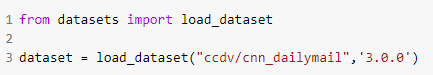
\includegraphics[scale=1]{SnippetCnnDailyMail.png}
\end{center}
Code à utiliser en ayant installé au préalable le module \textit{datasets} grâce à \textit{pip install datasets}.
\subsubsection{\textit{Dataset} XSUM}
$ _{} $ $ _{} $ $ _{} $ $ _{} $ $ _{} $Il s'agit d'un jeu de données de résumés de nouvelles avec des résumés gé\-né\-ra\-le\-ment qualifiés très abstraits. Ces données ont été constituées en collectant des articles en ligne de la \textit{BBC} (\textit{British Broadcasting Corporation}) qui sont accompagnés des petits résumés. Il s'agit d'un jeu de données en anglais donc. Plus précisément, chaque article est précédé d'une phrase d'introduction (appelée résumé) rédigée par un professionnel, généralement l'auteur de l'article. Le résumé porte la classe HTML "storybody introduction" et peut être facilement identifié et extrait du corps du texte principal. Ce \textit{dataset} a été introduit dans l'article \cite{XSumArticle} et tous les détails sur sa formation et ses spécificités peuvent y être trouvés.\\
En ce qui nous concerne, nous avons utilisé la version retrouvable sur \textit{hugging face} au \textit{chekpoint} éponyme \textbf{xsum} \footnote{\href{https://huggingface.co/datasets/xsum}{https://huggingface.co/datasets/xsum}}. Ce qui veut dire qu'il peut être chargé avec \textit{python} grâce aux lignes de code :
\begin{center}
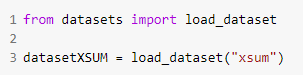
\includegraphics[scale=1]{SnippetXsum.png}
\end{center}
\subsubsection{\textit{Dataset} OrangeSum}
$ _{} $ $ _{} $ $ _{} $ $ _{} $ $ _{} $Ces données sont introduites à travers l'article \cite{eddine2020barthez} et ont été constituées en récupérant les contenus du site Web \textbf{Orange Actu}\footnote{\href{https://actu.orange.fr/}{https://actu.orange.fr/}}. Les pages scrappées couvrent presque une décennie, de février 2011 à septembre 2020. Elles appartiennent à cinq catégories prin\-ci\-pa\-les : France, monde, politique, automobile, et société . La catégorie société est elle-même divisée en 8 sous-catégories : santé, environnement, people, culture, médias, high-tech, insolite, et divers. Ce jeu de données est considéré comme l'équivalent en langue française du jeu de données \textit{XSum} en ce qui concerne le degré d'abstraction des résumés.\\
Pour ce mémoire, nous avons utilisé les données \textit{OrangeSum} tel que retrouvées sur le point d'entrée \textbf{GEM/OrangeSum} \footnote{\href{https://huggingface.co/datasets/GEM/OrangeSum}{https://huggingface.co/datasets/GEM/OrangeSum}}. Il peut donc être chargé identiquement que les 2 jeux de données précédents, \textit{XSum} et \textit{CNN/DailyMail}, en utilisant le nom de checkpoint \textit{GEM/OrangeSum}.
\subsubsection{\textit{Dataset} for-ULPGL-Dissertation}
Le jeu des données que nous avons dénommé \textbf{for-ULPGL-Dissertation} a été constitué par nous, à partir du sous-ensemble dénommé  \textit{abstract} du \textit{dataset} \textit{OrangeSum} mentionné dans la sous section précédente. Les données d'\textit{OrangeSum-Abstract} peuvent être chargées avec python en utilisant :
\begin{center}
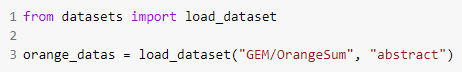
\includegraphics[scale=1]{SnippetOrangeAbstract.PNG}
\end{center}
A ces données, nous avons ajouté les quelques résumés jusque là générés grâce à notre système (dénommé \textbf{Mon Résumeur}). Plus exactement, la version actuelle (version $ 0.0.1 $ du $ 15/10/2022 $) de ce \textit{dataset} est constituée de $ 24 401 $ données en provenance d'\textit{OrangeSum-Abstract} et $ 450 $ données en provenance de \textbf{Mon Résumeur}. Soit environs $ 2\% $ du total en provenance de \textbf{Mon Résumeur}.\\
Nous ferons constamment évoluer ce \textit{dataset}, avec l'augmentation des résumés générés par notre système, de manière à ce qu'il soit ma\-jo\-ri\-tai\-re\-ment constitué des données jugées \textit{bonnes} par les utilisateurs de notre système.\\
Nous avons \textit{uploadé} le \textit{dataset} ainsi constitué dans notre compte \textit{hugging face}. Il y est pu\-bli\-que\-ment accessible et on peut y voir tous les détails sup\-plé\-men\-tai\-res \footnote{\href{https://huggingface.co/datasets/krm/for-ULPGL-Dissertation}{https://huggingface.co/datasets/krm/for-ULPGL-Dissertation}}. Comme il est au point d'entrée \textbf{krm/for-ULPGL-Dissertation}, on peut le charger avec \textit{Python} grâce aux bouts de code :
\begin{center}
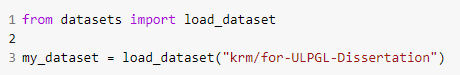
\includegraphics[scale=1]{SnippetMyDataset.PNG}
\end{center}

\subsection{Modèles utilisés pour la synthèse abstractive}
\subsubsection{Modèle BART optimisé}
$ _{} $ $ _{} $ $ _{} $ $ _{} $ $ _{} $Le modèle \textit{BART} \cite{BART} est celui que nous avons choisi comme modèle principal pour la synthèse abstractive dans notre système. Son objectif de pré-entraînement est assez général pour former un excellent modèle de langue comme nous l'avons décrit au chapitre précédent (voir le point \ref{BARTmodel}). Vu que notre système est destiné à fonctionner en production et non pas uniquement dans le monde de la recherche, il nous a été important de choisir une déclinaison de ce modèle adaptée à nos fins. C'est pour cela que nous avons choisi, pour notre système, d'utiliser la déclinaison accessible au \textit{checkpoint} \textbf{sshleifer/distilbart-cnn-12-6} finetuné pour la synthèse des textes. Ce \textit{transformer} peut être chargé très sim\-ple\-ment en utilisant le \textit{pipeline} traditionnel disponibilisé sur \textit{Hugging Face}\footnote{\href{https://huggingface.co/sshleifer/distilbart-cnn-12-6}{https://huggingface.co/sshleifer/distilbart-cnn-12-6}} par son auteur mais ce n'est pas très optimal de s'y prendre comme cela. C'est la raison pour laquelle, nous avons implémenté un \textit{pipeline} (comme on peut le voir sur la figure \ref{PipelineSumm}) nous permettant d'utiliser ce modèle de façon optimale, sans augmenter la complexité de calcul associée aux têtes d'attention de tous les modèles du type \textit{transformer} \cite{vaswani2017attention}. Les justifications des choix d'implémentation sont données au dernier point de ce chapitre.\\
Il faut noter que ce modèle est prévu exclusivement pour la langue anglaise.
\subsubsection{Modèle BARThez}
$ _{} $ $ _{} $ $ _{} $ $ _{} $ $ _{} $Le modèle \textit{BARThez} \cite{eddine2020barthez} est un modèle pré-entraîné sur du texte en français. Pour la synthèse abstractive, nous avons utilisé sa déclinaison finetunée sur le dataset \textit{OrangeSum} et disponible au \textit{checkpoint} \textbf{moussaKam/barthez-orangesum-abstract}. Néanmoins, on ne peut pas se contenter de ce modèle pour la synthèse en langue française car, étant donné le \textit{dataset} sur lequel il a été entraîné, la qualité de ses résumés n'est pas très satisfaisante quand on veut l'utiliser pour la production des résumés génériques sur des documents du type narratif et littéraire comme on le voudrait pour un système à usage général. En plus l'une des ses limitations est qu'il a une grande tendance à attribuer les propos des textes du résumé aux personnalités publiques actuelles quand bien même elles n'apparaissent pas dans le texte source (biais introduit par son \textit{dataset}). Les objectifs de pré-entraînement sont similaires à ceux du modèle \textit{BART}, donc il s'agit bien d'un modèle du type \textit{BART}. 
\subsubsection{Modèle mBARThez}
$ _{} $ $ _{} $ $ _{} $ $ _{} $ $ _{} $Le modèle \textit{mBARThez} est un modèle introduit dans l'article \cite{eddine2020barthez} (le même que celui de \textit{BARThez}) et basé sur \textbf{mBART}. Il s'agit d'un modèle pré-entraîné sur plusieurs langues et entraîné juste à prédire les mots masqués dans un texte. Nous l'avons finetuné pour pouvoir l'utiliser pour la synthèse automatique et espérer corriger avec le temps les faiblesses du modèle \textit{BARThez}. Pour le \textit{finetuning}, nous sommes parti du modèle \textit{mBARThez} re\-trou\-va\-ble au \textit{checkpoint} \textbf{moussaKam/mbarthez} \footnote{\href{https://huggingface.co/moussaKam/mbarthez}{https://huggingface.co/moussaKam/mbarthez}}.\\
Après entraînement de \textit{mBARThez}, nous avons produit un modèle pouvant être utilisé pour la synthèse (nous l'avons dénommé \textbf{BARTkrame-abstract}). 
\subsubsection{Modèle BARTkrame-abstract}
$ _{} $ $ _{} $ $ _{} $ $ _{} $ $ _{} $Il s'agit d'un modèle obtenu par \textit{finetuning} de \textit{mBARThez} sur notre \textit{dataset} dénommé \textit{for-ULPGL-Dissertation}. Cela nous a permis d'obtenir le \textit{checkpoint} \textbf{krm/BARTkrame-abstract} dont tous les détails sont accessibles sur la plateforme \textit{Hugging Face} où nous l'avons \textit{uploadé} \footnote{\href{https://huggingface.co/krm/BARTkrame-abstract}{https://huggingface.co/krm/BARTkrame-abstract}}.\\
$ _{} $ $ _{} $ $ _{} $ $ _{} $ $ _{} $En terme d'architecture, il s'agit d'un \textit{transformer} du type \textit{BART}, de même architecture que \textit{mBART}\cite{mBART_liu2020multilingual} car c'est ce qui a été utilisé comme modèle de base pour produire \textit{mBARThez} que nous avons finetuné enfin pour obtenir \textit{BARTkrame-abstract}.\\
C'est-à-dire qu'il s'agit d'un \textit{transformer} d'architecture exactement similaire à celle proposée à l'initial par \textit{Vaswani et al.} \cite{vaswani2017attention}  constitué de $ 12 $ couches dans l'encodeur et $ 12 $ dans le décodeur avec une dimension de $ 1024 $ \textit{tokens} pour le vecteur caché, sur $ 16 $ têtes d'attention.
\subsubsection{Modèle Pegasus}
$ _{} $ $ _{} $ $ _{} $ $ _{} $ $ _{} $Il s'agit de l'un des modèles jugés les plus performants pour les tâches de synthèse abstractive \cite{PEGASUSzhang2020pegasus}. En effet, son objectif de pré-entraînement est très proche d'une tâche de synthèse. Néanmoins, nous avons fini par le supprimer des modèles que nous rendons accessibles à travers notre \textit{API} à cause de sa lenteur et de sa taille. Cela est dû au fait que, du point de vu qualitatif, l'abstraction est parfois poussée trop loin de telle sorte que ce qui est dans la synthèse ne correspond pas vraiment à l'idée véhiculée par le texte source, le rapprochant beaucoup plus des systèmes de génération automatique des textes. Pour tirer ces conclusions, nous nous sommes servi du \textit{checkpoint} dénommé \textbf{google/pegasus-xsum} \footnote{\href{https://huggingface.co/google/pegasus-xsum}{https://huggingface.co/google/pegasus-xsum}}.
\subsection{Tests}
$ _{} $ $ _{} $ $ _{} $ $ _{} $ $ _{} $Nous avons mené plusieurs tests, à la fois sur les modèles abstractifs et sur les algorithmes de synthèse extractive de notre système. Les tests avaient pour objectif de démontrer le bien-fondé des techniques que nous avons choisi pour la synthèse automatique.\\
Nous avons utilisé comme métriques d'évaluation les mesures \textit{ROUGE-1}, \textit{ROUGE-2}, \textit{ROUGE-L} et une variante de cette dernière dénommée \textit{ROUGE-LSum} car il s'agit de loin des mesures les plus utilisées en synthèse automatique \cite{MaaliMnasri}.
\subsubsection{Tests sur les algorithmes de synthèse extractive}
$ _{} $ $ _{} $ $ _{} $ $ _{} $ $ _{} $Ce test a deux principaux objectifs :
\begin{itemize}
\item[-] choisir les poids à affecter aux divers algorithmes qui forment le système \textit{merging} (\ref{ArchiGlobExtract}).
\item[-] établir une mesure des performances de la partie qui fonctionne par combinaison des divers algorithmes de synthèse extractive (voir la figure \ref{ArchiGlobExtract} qui représente le système en question que nous avons nommé \textit{merging}) par rapport au module python dédié à la synthèse extractive, module dénommé \textit{gensim} (choisi principalement pour sa rapidité);
\end{itemize}
Le test a été effectué en se servant de $ 2 $ \textit{datasets} bien connus en synthèse automatique, à savoir \textit{CCN / DailyMail} et \textit{XSum}. Ce test a été mené en anglais pour ne pas avoir à traduire les \textit{datasets} et ainsi avoir des résultats les plus authentiques possible. Pour chacun de ces \textit{datasets}, nous avons réalisé nos expérimentations sur les données de test. Nous avons choisi ces deux \textit{datasets} car ils sont en quelques sortes complémentaires. En effet, \textit{CCN / DailyMail} est essentiellement extractif tandis que \textit{XSum} est beaucoup plus abstractif \cite{eddine2020barthez}.
\subsubsection{Tests sur BART et BART optimisé}
$ _{} $ $ _{} $ $ _{} $ $ _{} $ $ _{} $Ce test avait pour objectif d'évaluer les performances du modèle \textit{BART} quand on l'utilise à travers le pipeline implémenté par nous selon la figure \ref{PipelineSumm} par rapport à une utilisation classique (selon le pipeline classique \cite{GRAAL_HF_tunstall2022natural}). Nous avons pour cela utilisé les \textit{datasets}
\textit{CCN / DailyMail} et \textit{XSum} sur le \textit{checkpoint} dénommé \textit{sshleifer/distilbart-cnn-12-6} que nous avons utilisé comme modèle \textit{BART} dans l'ensemble du système. 
\subsubsection{Précisions sur l'entraînement et les tests de BARTKrame-abstract}
$ _{} $ $ _{} $ $ _{} $ $ _{} $ $ _{} $La version actuelle de ce modèle (le $ 16/10/2022 $, version $ 0.0.1 $) a été obtenue après entraînement de \textit{mBARThez} avec \textbf{$  5000 $ données d'entraînement et $ 100 $ données de validation} provenant du \textit{dataset} \textit{for-ULPGL-Dissertation} (le nombre de données a été réduit suite aux limitations en terme de ressources matérielles dont nous disposions). Nous avons utilisé, pour cet entraînement, un environnement sur \textit{google colab}\footnote{\href{https://colab.research.google.com/}{https://colab.research.google.com/}} équipé d'un \textit{GPU} et à présent l'entraînement a été fait sur $ 12 $ époques et a duré $ 8 $ heures. Les hy\-per\-pa\-ra\-mè\-tres utilisés peuvent être ainsi présentés :
\begin{itemize}
\item[•] \textit{Learning rate initial :} $ 5.6*10^{-6} $;
\item[•] Taille des batchs (\textit{batch size}) : 4;
\item[•] Optimiseur : \textit{Adam} (avec $ \beta = 0.999 $ et $ \epsilon = 1*10^{-8} $)
\item[•] Le \textit{Learning rate} était à décroissance linéaire;
\item[•] Le grain de sélection aléatoire des données était de $ 42 $;
\item[•] Métrique : \textit{ROUGE}.
\end{itemize}
Pour plus d'informations sur notre modèle et le processus d'entraînement, se rapporter à son dépôt sur \textit{Hugging Face}\footnote{\href{https://huggingface.co/krm/BARTkrame-abstract}{https://huggingface.co/krm/BARTkrame-abstract}}.\\
Le test réalisés sur ce modèle ont été faits sur le dataset \textit{for-ULPGL-Dissertation} car notre objectif est d'obtenir un modèle principalement en français. Une partie des résultats de test a été obtenue immédiatement après entraînement (c'est-à-dire sur les données de validation) et nous avons réalisé après cela un autre test sur les données de test de notre \textit{dataset}.

\subsection{Résultats des tests}
Pour ces résultats, il faut noter que plus une mesure est supérieure, plus le modèle a de chance de donner des résultats de bonne qualité. Ce n'est pas toujours le cas mais la mesure \textit{ROUGE} ici utilisée est un excellent indicateur des performances d'un système de résumé automatique (voir la section \ref{sectionSurROUGE}).
\subsubsection{Algorithmes de synthèse extractive}
\begin{itemize}
\item[1°)] \textbf{Recherche des poids des modèles constituant \textit{merging}}\\
Pour cet essai, il nous a d'abord fallu évaluer la confiance que nous pouvons accorder à chaque modèle constituant \textit{merging}. Ce que nous appelons \textit{merging} est formé, comme on peut le voir sur la figure \ref{ArchiGlobExtract} par les algorithmes de synthèse extractive suivants : \textit{TF-IDF}, \textit{LSA}, \textit{Heuristiques}, \textit{TextRank}, \textit{LexRank} et \textit{Luhn}. Pour la recherche des poids, nous avons considéré uniquement les résultats des tests sur le \textit{dataset} \textit{CNN/DailyMail} car il est plus adapté à la synthèse extractive. Les résultats ont été les suivants :
\begin{center}
\captionof{table}{Résultats ROUGE des algorithmes de \textit{merging} sur \textit{CNN/DailyMail}}
\label{SumyOnCnn}
\setlength{\arrayrulewidth}{1pt}
\definecolor{gris}{gray}{0.65}
\begin{tabular}{|p{4cm}||p{2.5cm}|p{2.5cm}|p{2.5cm}|p{2.5cm}|}
\hline
\cellcolor{gris}\textbf{Algorithmes} & R-1  & R-2 & R-L & R-LSum \\
\hline
\hline
\textbf{Heuristique} & $ 24.72 $  & $ 7.95 $  & $ 16.44 $ & $ 19.64 $ \\
\hline
\textbf{LexRank} & $ 22.88 $ & $ 5.88 $  & $ 15.02 $ & $ 18 $ \\
\hline
\textbf{TextRank} & $ 19.91 $ & $ 5.06 $ & $ 13.52 $ & $ 16.13 $ \\
\hline
\textbf{LSA} & $ 20.43 $ & $ 3.68 $ & $ 12.84 $ & $ 15.70 $ \\
\hline
\textbf{Luhn} & $ 19.66 $ & $ 4.79 $ & $ 12.66 $ & $ 15.39 $ \\
\hline
\textbf{Tf-Idf} & $ 10.98 $ & $ 1.99 $ & $ 7.77 $ & $ 8.95 $ \\
\hline
\end{tabular}
\end{center}
Pour la recherche des poids, nous avons appliqué une méthode heuristique simple. En vertu des résultats que nous avons dans le tableau \ref{SumyOnCnn}, nous avons accordé les scores $ 1 $, $ 2 $, $ 3 $, $ 4 $, $ 5 $ et $ 6 $ respectivement aux algorithmes \textit{Tf-Idf}, \textit{Luhn}, \textit{LSA}, \textit{TextRank}, \textit{LexRank} et \textit{Heuristique} comme ils se suivent dans le tableau. Ensuite, nous avons normalisé ces poids en appliquant une fonction \textit{softmax} à cet ensemble de rangs. Donc, en appliquant $ e^{i}/\left( \sum_{n=1}^{6} e^{n}\right) $ pour tout $ i\in \left\lbrace 1, 2, 3, 4, 5, 6\right\rbrace $ nous avons trouvé les poids suivants :\newpage
\begin{center}
\captionof{table}{Poids des algorithmes constituant \textit{merging}}
\label{MergingWeights}
\setlength{\arrayrulewidth}{1pt}
\definecolor{gris}{gray}{0.65}
\begin{tabular}{|p{2.4cm}|p{2.4cm}|p{2.4cm}|p{2.4cm}|p{2.4cm}|p{2.4cm}|}
\hline
 \textbf{Heuristique} & \textbf{LexRank}  & \textbf{TextRank} & \textbf{LSA} & \textbf{Luhn}  & \textbf{Tf-Idf} \\
\hline
\hline
 0.633 & 0.233  & 0.0857 & 0.0315 & 0.0116  & 0.0042 \\
\hline
\end{tabular}
\end{center}
\item[2°)] \textbf{Comparaison quantitative de Merging avec Gensim}\\
L'évaluation de ces deux modèles sur \textit{CNN/DailyMail}, en se servant des poids listés dans le tableau \ref{MergingWeights}, a donné les résultats suivants :
\begin{center}
\captionof{table}{Comparaison des algorithmes Gensim et \textit{merging} sur \textit{CNN/DailyMail}}
\label{MergingVsGensimOnCNN}
\setlength{\arrayrulewidth}{1pt}
\definecolor{gris}{gray}{0.65}
\begin{tabular}{|p{4cm}||p{2.5cm}|p{2.5cm}|p{2.5cm}|p{2.5cm}|}
\hline
\cellcolor{gris}\textbf{Algorithmes} & R-1  & R-2 & R-L & R-LSum \\
\hline
\hline
\textbf{Gensim} & $ 31.74 $  & $ 12.28 $  & $ 20.69 $ & $ 27.70 $ \\
\hline
\textbf{Merging} & $ 23.19 $ & $ 6.70 $  & $ 15.05 $ & $ 18.17 $ \\
\hline
\end{tabular}
\end{center}
L'évaluation de ces deux modèles sur \textit{XSum}, en se servant des poids listés dans le tableau \ref{MergingWeights}, a quant à elle donné les résultats suivants :
\begin{center}
\captionof{table}{Comparaison des algorithmes Gensim et \textit{merging} sur \textit{XSum}}
\label{MergingVsGensimOnXSum}
\setlength{\arrayrulewidth}{1pt}
\definecolor{gris}{gray}{0.65}
\begin{tabular}{|p{4cm}||p{2.5cm}|p{2.5cm}|p{2.5cm}|p{2.5cm}|}
\hline
\cellcolor{gris}\textbf{Algorithmes} & R-1  & R-2 & R-L & R-LSum \\
\hline
\hline
\textbf{Gensim} & $ 15.10 $  & $ 2.50 $  & $ 10.13 $ & $ 11.29 $ \\
\hline
\textbf{Merging} & $ 14.90 $ & $ 1.88 $  & $ 10.09 $ & $ 10.12 $ \\
\hline
\end{tabular}
\end{center}
\end{itemize}
\subsubsection{Résultats de BART en usage normal puis en usage optimisé}
Les tests sur le jeu des données \textit{CNN/DailyMail} ont donné les résultats suivants :
\begin{center}
\captionof{table}{Comparaison de BART avec BART optimisé sur \textit{CNN/DailyMail}}
\label{BARTvsBARToptCNN}
\setlength{\arrayrulewidth}{1pt}
\definecolor{gris}{gray}{0.65}
\begin{tabular}{|p{5cm}||p{2.5cm}|p{2.5cm}|p{2.5cm}|p{2.5cm}|}
\hline
\cellcolor{gris}\textbf{Algorithmes} & R-1  & R-2 & R-L & R-LSum \\
\hline
\hline
\textbf{BART optim.} & $ 43.72 $  & $ 20.22 $  & $ 30.06 $ & $ 36.62 $ \\
\hline
\textbf{BART normal} & $ 36.66 $ & $ 14.31 $  & $ 25.88 $ & $ 31.038 $ \\
\hline
\end{tabular}
\end{center}
Et les tests sur le jeu des données \textit{XSum} ont donné :
\begin{center}
\captionof{table}{Comparaison de BART avec BART optimisé sur \textit{XSum}}
\label{BARTvsBARToptXSum}
\setlength{\arrayrulewidth}{1pt}
\definecolor{gris}{gray}{0.65}
\begin{tabular}{|p{5cm}||p{2.5cm}|p{2.5cm}|p{2.5cm}|p{2.5cm}|}
\hline
\cellcolor{gris}\textbf{Algorithmes} & R-1  & R-2 & R-L & R-LSum \\
\hline
\hline
\textbf{BART optim.} & $ 20.57 $  & $ 3.50 $  & $ 13.42 $ & $ 13.41 $ \\
\hline
\textbf{BART normal} & $ 17.67 $ & $ 2.66 $  & $ 12.08 $ & $ 12.091 $ \\
\hline
\end{tabular}
\end{center}

\subsubsection{Résultats des tests de BARTKrame-abstract}
Les tests sur le jeu des données \textit{for-ULPGL-Dissertation} ont donné les résultats suivants:
\begin{center}
\captionof{table}{Résultats de test de \textit{BARTkrame-abstract} sur \textit{for-ULPGL-Dissertation} }
\label{ResultBARTkrame-abstract}
\setlength{\arrayrulewidth}{1pt}
\definecolor{gris}{gray}{0.65}
\begin{tabular}{|p{5cm}||p{2.5cm}|p{2.5cm}|p{2.5cm}|p{2.5cm}|}
\hline
\cellcolor{gris}\textbf{Données} & R-1  & R-2 & R-L & R-LSum \\
\hline
\hline
\textbf{Validation} & $ 27.03 $  & $ 13.34 $  & $ 23.92 $ & $ 24.19 $ \\
\hline
\textbf{Test} & $ 24.08 $ & $ 7.28 $  & $ 19.30 $ & $ 19.29 $ \\
\hline
\end{tabular}
\end{center}

\textbf{Il faudra noter que le dataset utilisé pour entraîner ce modèle, ainsi que le modèle lui-même, seront entrain d'être améliorés. Pour avoir les résultats actualisés au-delà de la date de soumission de ce document, il faut se rapporter à leurs liens (dépôts HuggingFace sus-mentionnés pour \textit{BARTkrame-abstract} et pour \textit{for-ULPGL-Dissertation}).}
\subsection{Interprétation des résultats}
\subsubsection{Système de synthèse extractive}
$ _{} $ $ _{} $ $ _{} $ $ _{} $ $ _{} $Comme on peut le voir dans les tableaux \ref{MergingVsGensimOnCNN} et \ref{MergingVsGensimOnXSum}, les performances du module python \textit{gensim} demeurent supérieures à celles de \textit{merging}. Cela est un fait, du point de vu quantitatif. Néanmoins, comme pourra en juger le lecteur au vu des exemples mis en annexe, cela n'est pas complètement vrai du point de vu qualitatif.\\
$ _{} $ $ _{} $ $ _{} $ $ _{} $ $ _{} $En effet, le modèle \textit{merging} tel que nous l'avons implémenté gère mieux le ratio entré par l'utilisateur et est moins sensible aux problèmes introduits par les sauts de ligne arbitraires dans le texte. Également, \textit{merging} repère très bien les éléments saillants du texte (voir l'annexe \ref{AnnexesExemples}) .\\
$ _{} $ $ _{} $ $ _{} $ $ _{} $ $ _{} $Il faut finalement constater que les mesures sur \textit{XSum} sont toujours inférieures à celles faites sur \textit{CNN/DailyMail}. Cela est très normal et justifié par le fait que le \textit{dataset} \textit{CNN/DailyMail} est essentiellement du type extractif alors que \textit{XSum} est du type \textit{abstractif}.
\subsubsection{BART et BART optimisé}
$ _{} $ $ _{} $ $ _{} $ $ _{} $ $ _{} $Comme on peut le voir au travers des tableaux \ref{BARTvsBARToptCNN} et \ref{BARTvsBARToptXSum}, les résultats obtenus avec le modèle \textit{BART} en usage optimal sont largement supérieurs à ceux obtenus en usage classique (normale). Le test sur \textit{CNN/DailyMail} donne des résultats sans équivoque sur la supériorité de \textit{BART optimisé} par rapport au \textit{BART classique}. Néanmoins, les résultats sur \textit{XSum} sont proches (comme on le voit dans le tableau \ref{BARTvsBARToptXSum}) et cela est bien évident car, comme \textit{XSum} est formé des résumés à tendance plus abstraite et que le modèle \textit{BART} est la base de ces deux implémentations (classique et optimisée), aucune ne devait dépasser un certain seuil en ce qui concerne la ressemblance à \textit{XSum}. En plus, la mesure \textit{ROUGE} est incapable de repérer les similarités sémantiques quand des tournures différentes sont utilisées. Néanmoins, l'utilisation de la mesure \textit{ROUGE} sur un \textit{dataset} à tendance abstractive est un bon indicateur de la fidélité du modèle au texte d'origine quand il s'agit d'un modèle abstractif.
\subsubsection{Commentaires sur les résultats de BARTkrame-abstract}
$ _{} $ $ _{} $ $ _{} $ $ _{} $ $ _{} $Les résultats obtenus sur \textit{BARTkrame-abstract} ne devaient pas différer assez sur les données de validation par rapport aux données de test car les données proviennent d'un même \textit{dataset} et, comme le \textit{dataset} a été constitué par un choix aléatoire des données à affecter aux différentes catégories (\textit{train}, \textit{test} et \textit{validation}), les caractéristiques statistiques des données de validation sont approximativement les mêmes que celles des données de test. Cela devait suffire pour assurer que les résultats obtenus sur les données de test et ceux obtenus sur les données de validation soient assez proches.\\
$ _{} $ $ _{} $ $ _{} $ $ _{} $ $ _{} $La signification des résultats du tableau \ref{ResultBARTkrame-abstract} est simplement que le modèle est encore très sensible à des petites variations. Donc il n'est pas encore stable et l'entraînement doit être poursuivi. Cela est évidemment clair quand on regarde les résultats qualitatifs (les synthèses) obtenus en utilisant ce modèle dans notre système. On peut voir en effet que le modèle parvient à capturer les points importants mais ne parvient pas encore à repérer clairement où s'arrêter, voir l'annexe \ref{AnnexesExemples}.

\section{Justification des choix d'implémentation}
$ _{} $ $ _{} $ $ _{} $ $ _{} $ $ _{} $Voici donc quelques justifications très sommaires des choix d'implémentation que nous avons faits. Les points saillants sont principalement ici présentés :
\begin{itemize}
\item[•] L'un des modules utilisés pour la synthèse extractive est \textit{gensim}. Nous l'avons prin\-ci\-pa\-le\-ment choisi comme algorithme de base de la synthèse extractive suite à sa rapidité. Il implémente néanmoins l'algorithme \textit{Tf-Idf} avec quelques optimisations \cite{srinivasaGENSIMnatural}.
\item[•] Pour le module mélangeant un grand nombre d'algorithmes utilisés pour la synthèse extractive, nous avons opté pour cette approche car nous sommes partis de l'idée selon laquelle, du point de vu qualitatif, une synthèse qui serait générée en prenant en compte divers aspects serait plus susceptible d'être riche que les autres. Bien que les résultats quantitatifs (mesure \textit{ROUGE}) n'ont pas été très satisfaisants, nous estimons avoir eu raison d'implémenter ces algorithmes au vu de la valeur ajoutée en terme qualitatif comme on peut en juger grâce aux synthèses mises à l'annexe \ref{AnnexesExemples}.
\item[•] Pour la synthèse abstractive, le fait de tourner notre choix vers les modèles du type \textit{BART} a été inspiré par la nécessité de réaliser des synthèses abstraites mais pas trop pour ne pas s'éloigner du contenu du texte source. Cela nous a amené à exclure \textit{PEGASUS} bien que ce soit l'un des modèles les mieux cotés en synthèse abstractive. En fait, \textit{PEGASUS} s'éloigne souvent des vraies idées véhiculées par le texte source. En plus, étant donné que le modèle \textit{BART} est moins pesant et plus manipulable que le modèle \textit{T5}, il a été l'unique à considérer (comme \textit{PEGASUS} et \textit{T5} étaient \textit{ipso facto} exclus).
\item[•] Comme point de repère avec les modèles complètement conçus en français, nous avons utilisé \textit{BARThez} car c'est la référence française en ce qui concerne les \textit{tranformers} de type encodeur-décodeur.
\item[•] Pour l'entraînement de notre modèle, nous sommes parti de \textit{mBARThez} qui est à la base un modèle \textit{mBART} dont le pré-entraînement a été poursuivi en insérant une grande masse des données en français \cite{eddine2020barthez}. Comme nous devions réaliser le \textit{finetuning} sur du texte en français pour obtenir un modèle complètement en français, nous estimons que c'est l'approche la plus appropriée et devant nous permettre de partir d'un modèle de langue déjà très bon en français. Ce dernier fait a pour avantage de nous permettre de diminuer les données d'entraînement.
\item[•] Pour l'implémentation de l'\textit{API}, nous avons choisi d'utiliser \textit{Flask} étant donné qu'il donne une grande liberté aux développeurs. Il n'a pas une structure préconçue et imposante.
\item[•] L'utilisation de \textit{ReactJS} pour la partie client a été motivée par sa popularité, mais également nous nous sentons plus à l'aise avec la syntaxe et l'architecture de ce \textit{framework}.
\item[•] Concernant le fait de réaliser une \textit{API} parfaitement distinguée, l'objectif est de permettre l'implémentation, par divers développeurs, de toute forme de systèmes pouvant en utiliser les services, participant par la même occasion à l'amélioration de notre modèle de synthèse. C'est d'ailleurs la raison pour laquelle nous avons également donné aux utilisateurs la possibilité d'évaluer les résumés qu'ils obtiennent. Cela constituera en fait un écosystème d'annotation des résumés par des humains.
\end{itemize}
\section{Conclusion partielle}
$ _{} $ $ _{} $ $ _{} $ $ _{} $ $ _{} $Dans ce chapitre, qui est le dernier de notre travail, nous venons de finaliser la conception de notre système. Cela nous a permis de montrer que le système a une ar\-chi\-tec\-tu\-re \textit{3-tiers} classique, avec une petite base des données qui nous permet également de récolter les données de synthèse pouvant par la suite s'utiliser pour améliorer les modèles de \textit{machine learning} dédiés à la synthèse automatique des documents.\\
Nous y avons également présenté les diverses métriques couramment utilisées pour l'é\-va\-lua\-tion des systèmes de synthèse automatique, tout en utilisant le paquet \textit{ROUGE} qui est la métrique la plus utilisée pour cette fin.\\
$ _{} $ $ _{} $ $ _{} $ $ _{} $ $ _{} $Ce chapitre nous a non seulement permis de décrire complètement l'implémentation de notre système mais également, il nous a permis de montrer que le modèle \textit{BART} tel que nous l'avons utilisé pour la synthèse abstractive est plus performant que si on l'utilisait dans une pipeline classique. Nous avons également montré que les résultats du module \textit{gensim} pour la synthèse automatique sont meilleurs que ceux de l'algorithme \textit{merging}, mais que ce dernier est qua\-li\-ta\-ti\-ve\-ment très satisfaisant et plus robuste aux variations mineures dans les textes. Nous avons également montré que le modèle \textit{BARTkrame-abstract}, qui a été obtenu après \textit{finetuning} de \textit{mBARThez} (un modèle basé sur \textit{mBART}) sera entrain d'être amélioré au fil de l'utilisation du système, étant donné que tout l'ensemble a été conçu en tenant compte de cet aspect.
\chapter*{CONCLUSION GÉNÉRALE}\addcontentsline{toc}{chapter}{CONCLUSION GÉNÉRALE}
$ _{} $ $ _{} $ $ _{} $ $ _{} $ $ _{} $Ce travail est un rapport accompagnant le système que nous avons mis au point en guise de mémoire. Le système en question a pour rôle de générer automatiquement les résumés des documents qui lui sont fournis.

Au début de ce travail, nous avons fait quelques hypothèses. Dans la première hypothèse, nous affirmons qu'un traitement purement linguistique ne suffirait pas pour pouvoir produire des résumés performants en utilisant un système informatique. A l'issu de nos recherches, et des expérimentations, nous avons pu vérifier cette hypothèse car, nous avons démontré que le traitement purement linguistique du langage naturel est très gour\-mand en ressources et très fastidieux. En plus, le langage naturel n'est pas aussi précis que peut l'être un langage formel quelconque.\\
$ _{} $ $ _{} $ $ _{} $ $ _{} $ $ _{} $A la seconde hypothèse, nous avons avancé qu'on ne peut se passer de l'intelligence artificielle si on veut obtenir des systèmes de résumé de performance presqu'humaine. Cela se vérifie à travers la littérature que nous avons présentée, ainsi que la complexité inhérente au traitement du langage naturel tel que nous l'avons montré dans ce travail. L'usage de l'intelligence artificielle permet de réaliser des tâches à grande complexité à un coût faible par rapport à une approche algorithmique détaillée.\\
$ _{} $ $ _{} $ $ _{} $ $ _{} $ $ _{} $La troisième et dernière hypothèse que nous avons émise était qu'une architecture du type \textit{transformer}, à laquelle on joint des traitements lin\-guis\-ti\-ques sommaires comme la segmentation du texte par exemple, permettrait d'obtenir des bons systèmes de résumé automatique. Cette hypothèse doit être précisée au vu des études que nous avons menées à travers ce travail. En effet, les recherches que nous avons menées nous ont permis de nous rendre compte que, pour des systèmes destinés à un usage en production, il est mieux de se limiter aux algorithmes classiques pour la synthèse extractive au lieu d'utiliser des systèmes d'intelligence artificielle très lourds. Cela permet de gagner en performance et en expérience utilisateur. Néanmoins, grâce aux modèles de \textit{deep learning} basés sur les mécanismes d'attention (les \textit{transformers} en l'occurence), on peut se passer de la nécessité d'implémenter explicitement les règles lin\-guis\-ti\-ques car le pré-entraînement des \textit{transformers} capture déjà les règles de la langue considérée. Ainsi, les règles linguistiques à implémenter peuvent être réduites au strict minimum. C'est pour cela que, bien que les modèles soient assez lourds en général, ils sont incontournables si on veut obtenir des résumés de qualité presqu'humaine (abstractifs), et corriger les erreurs de coupure de sens inhérentes à la synthèse par sélection brute des phrases saillantes (extraction). Ainsi donc, nous avons montré qu'on ne peut se passer des modèles d'intelligence artificielle si on veut obtenir des systèmes de résumé automatique performants, surtout que tous les aspects du langage naturel ne peuvent pas être formalisés.\\
$ _{} $ $ _{} $ $ _{} $ $ _{} $ $ _{} $L'objectif de ce travail était, comme énoncé dans l'introduction générale, de concevoir et réaliser un système, en l'occurrence une application web, devant permettre la génération automatique des résumés des textes. Pour atteindre ledit objectif, il nous a fallu réaliser $ 6 $ objectifs spécifiques.\\
$ _{} $ $ _{} $ $ _{} $ $ _{} $ $ _{} $Le premier objectif, concernant l'évaluation des failles et limites des techniques de synthèse existantes a été mené à terme. Il a débouché sur le constat selon lequel, les systèmes de résumé extractif par usage d'algorithmes classiques (sans traitement intelligent) sont couramment utilisés à cause de la facilité d'implémentation mais sont sujets aux erreurs de coupure de sens, étant donné que les phrases saillantes sont sélectionnées en les enlevant de leur contexte initial. Ce problème peut être réduit en essayant d'exclure au maximum les éléments hors contexte. Malheureusement, cette dernière manipulation a ses limites car elle ne peut pas supprimer complètement les coupures de sens inhérents au processus même de synthèse extractif. C'est pourquoi, les modèles abstractifs se présentent comme modèle de choix pour résoudre ce problème. Nous avons également montré que, comme le module \textit{gensim} de python a moins de chance de capturer un large éventail des points saillants dans les textes, l'utilisation d'un algorithme qui combinerait plusieurs approches de synthèse extractive a plus de chances de capturer une multitudes d'aspects. C'est pourquoi nous avons implémenté un algorithme de synthèse extractive fonctionnant par combinaison de divers algorithmes qui ont chacun sa spécificité. Cela a contribué à une nette amélioration qualitative sur les résultats, ce qui fait partie du second objectif de ce travail qui consistait à corriger le cas échéant, les failles observées.\\
$ _{} $ $ _{} $ $ _{} $ $ _{} $ $ _{} $Et, s'agissant justement de ce second objectif, qui consiste à apporter les améliorations nécessaires, nous devons préciser que, pour la synthèse abstractive, que nous avons réalisé grâce aux modèles du type \textit{transformer}, nous avons implémenté un pipeline qui permet de réaliser la synthèse des très longs documents (allant au-delà de $ 100 $ pages) alors qu'au préalable, les \textit{transformers} utilisés se limitent à environ $ 1 $ page.\\
$ _{} $ $ _{} $ $ _{} $ $ _{} $ $ _{} $Le troisième objectif consistant à établir une architecture logique fonctionnelle et optimale pour obtenir des synthèse de qualité a été atteint, d'abord à travers l'optimisation que nous avons faite durant l'usage du modèle \textit{BART} pour la synthèse abstractive (et cela contribue également au second objectif du travail), puis à travers l'architecture globale que nous avons utilisé pour notre système. Il s'agit en fait d'une architecture \textit{3-tiers} classique mais qui est in\-trin\-sè\-que\-ment évolutive étant donné la séparation nette faite entre \textit{API} et \textit{client web}, auquel on joint un stockage continu des résumés obtenus.\\
$ _{} $ $ _{} $ $ _{} $ $ _{} $ $ _{} $On conclut, de ce qui  vient d'être mentionné, que le quatrième objectif, consistant à élaborer une \textit{API} devant servir de moteur de résumé a également été atteint, ainsi que le très important cinquième objectif consistant à mettre au point une base des données devant nous permettre de constituer à la longue un \textit{dataset} riche, susceptible d'être utilisé pour élaborer des modèles de résumé de plus en plus performants.\\
$ _{} $ $ _{} $ $ _{} $ $ _{} $ $ _{} $Le sixième et dernier objectif de ce travail, consistant à mettre au point une interface web devant consommer les services de l'\textit{API} a également été atteint au vu du système que nous avons réalisé.\\
Les $ 6 $ objectifs spécifiques ayant été atteints, nous estimons avoir mis au point un écosystème complet de synthèse automatique des documents.\\
$ _{} $ $ _{} $ $ _{} $ $ _{} $ $ _{} $Nous devons néanmoins préciser que ce système est mieux adapté à la synthèse générique des documents de type narratif, argumentatif et littéraire en général (romans, nouvelles, discours, articles de presse, documents à faible densité mathématique et figures,...).\\
Pour la synthèse extractive, nous avons utilisé deux approches comme nous l'avons déjà mentionné (le module \textit{gensim} de python et \textit{merging} que nous avons mis au point en combinant plusieurs méthodes de synthèse extractive).\\
$ _{} $ $ _{} $ $ _{} $ $ _{} $ $ _{} $Pour la synthèse abstractive, celle qui se rapproche le plus de la synthèse humaine, nous avons utilisé des modèles du type \textit{BART}, pour éviter de pousser trop loin l'abstraction comme le ferait \textit{PEGASUS}, et en même temps éviter d'utiliser un modèle inutilement trop général pour notre contexte, comme c'est le cas du modèle \textit{T5}.\\
$ _{} $ $ _{} $ $ _{} $ $ _{} $ $ _{} $Nous avons également mis en place un \textit{dataset} de résumé automatique que nous avons nommé \textit{for-ULPGL-Dissertation} qui accueillera au fil du temps les données de synthèse recueillies à travers la base des données de notre système (que nous avons nommé \textit{Mon Résumeur}) et deviendra de plus en plus riche et performant. Ce \textit{dataset}, dans sa version actuelle (pas encore très riche) a été utilisé pour mettre au point le modèle \textit{BATkrame-abstract} basé sur le modèle \textit{mBARThez}, lui-même basé sur \textit{mBART} que nous continuerons également à améliorer en même temps que le \textit{dataset}. Finalement, nous avons utilisé le paquet \textit{ROUGE} comme métrique d'évaluation de notre système.\\

Ce domaine est très intéressant et surtout très vaste, c'est pourquoi l'ouverture de ce sujet est très large. Ainsi, aux futurs étudiants, qui comptent améliorer ce travail ou tout simplement œuvrer dans le même domaine, nous pouvons suggérer :
\begin{itemize}
\item[•] d'implémenter, selon leurs besoins, d'autres clients web pouvant consommer les services de cette \textit{API} mise au point;
\item[•] d'étudier minutieusement les limites de la métrique \textit{ROUGE} ainsi que d'autres métriques d'évaluation des systèmes génératifs pour mettre au point, le cas échéant, des nouvelles métriques, aussi moins gourmandes en ressources que \textit{ROUGE} mais plus performantes en matière d'évaluation de qualité;
\item[•] d'étendre notre système de résumé automatique au \textit{résumé guidé} et multi-documents;
\item[•] d'étendre le processus au résumé des vidéos ou même d'audios tout simplement;
\item[•] d'étudier la possibilité de mise au point des systèmes devant permettre la synthèse des documents à forte teneur mathématique;
\item[•] d'étudier la possibilité de réaliser un résumeur universel, c'est-à-dire qui serait adapté à la majorité de types de documents connus (documents spécialisés, littéraires,...);
\item[•] d'optimiser le temps de calcul des modèles de synthèse automatique;
\item[•] etc
\end{itemize}
\backmatter
%\appendix
\begin{appendices}
\section{Algorithme de traitement brut}\label{Anne1}
\input{Filtre1}
\section{Algorithme de traitement par blocs}\label{Anne2}
\input{Filtre2}
\end{appendices}
\bibliographystyle{acm}
\bibliography{Bibliographie}
\end{document}